\documentclass[12pt]{article}
\usepackage{graphicx,subfigure}
\usepackage{hyperref,amsmath,fancyhdr}
\usepackage[usenames,dvipsnames]{color}
\usepackage{supertabular, listings}
\usepackage[english]{babel} 
%\usepackage[left=2.0cm, right=2.0cm, top=2.5cm, bottom=2.5cm, headsep=1.2cm]{geometry}
\usepackage{amscd,amssymb,verbatim}
%\usepackage[TS1,OT1,T1]{fontenc}
\usepackage{cite}
\usepackage{eurosym}
\usepackage{array}
\usepackage{hyperref}
\usepackage{fancyvrb}
\usepackage{multirow}
\usepackage[titletoc]{appendix}
%\usepackage{ccaption}
\pagestyle{headings}
\usepackage{subfigure} 
\usepackage{color}
\usepackage{spverbatim}
 
 
\textheight 23cm
\textwidth 17.5cm
\topmargin -1.0cm
\hoffset -2.0cm

%\newfixedcaption{\figcaption}{figure}

\begin{document}

\begin{titlepage}
\centering
{{\Huge\bf \sffamily MINT}}\\
\vspace{0.35cm}
{{\Huge\bf \sffamily version 1.0}}\\
\vspace{0.5cm}
{{\Huge\bf \sffamily Users' Manual}}\\
\vspace{1cm}
{\large{\bf{\sffamily Anna G\'{o}rska}}}\\
{\large{\bf{\sffamily Maciej Jasi\'{n}ski}}}\\
{\large{\bf{\sffamily Joanna Trylska}}}\\
\vspace{2cm}

\includegraphics[width=0.4\textwidth]{./pictures/Mint.png}\\
\vspace{0.2cm}

\includegraphics[width=0.3\textwidth]{./pictures/logoLMB.png}
\end{titlepage}
\newpage
     {\sffamily{MINT is a free software; you can redistribute it and/or modify 
     it under the terms of the GNU General Public License version 2,  
     as published by the Free Software Foundation.\\
     \\                                                                       
     This program is distributed in the hope that it will be useful,        
     but WITHOUT ANY WARRANTY; without even the implied warranty of       
     MERCHANTABILITY or FITNESS FOR A PARTICULAR PURPOSE.  See the GNU General Public License for more details.\\                          
     \\                                                                       
     You should have received a copy of the GNU General Public License    
     along with this program; if not, write to the                         
     Free Software Foundation, Inc.,                                      
     59 Temple Place - Suite 330, Boston, MA  02111-1307, USA.\\
     \\
     \vspace*{1cm}
     Copyright (C) 2013 -- 2014: University of Warsaw}}  
\includegraphics[width=0.1\textwidth]{./pictures/logoUW.png}

\newpage
\tableofcontents
\newpage
\newcommand*{\elem}[1]{{\color{Gray}{\tt{<#1>}}}}
\newcommand*{\greyT}[1]{{\color{Gray}{\tt{#1}}}}

\section{Introduction}
{\tt MINT} (Motif Identifier for Nucleic acids Trajectory) is an automatic tool for reading and analyzing three-dimensional structures of nucleic acids, their molecular dynamics trajectories (written in CHARMM, Gromacs, NAMD, LAMMPS, or Amber formats) or other conformation sets.\\

\noindent
{\tt MINT} deals with both DNA and RNA molecules. However, since mainly RNAs acquire complicated 3D folds, we write this manual in the context of RNA. The analysis includes hydrogen bonding, stacking and secondary-structural motifs. For many conformations of the same nucleic acid molecule {\tt MINT} provides various physicochemical properties as a function of simulation time (or frame), as well as statistics providing an overall-view of the changes in these properties occuring in the inputted conformation set (e.g., trajectory).\\

\noindent
Please direct your comments and questions about the MINT package to:\\
{\tt{agorska@cent.uw.edu.pl}} or {\tt{m.jasinski@cent.uw.edu.pl}}\\
Centre of New Technologies,
University of Warsaw\\
Banacha 2c, 02-097 Warsaw, Poland\\
phone:  $+$48 22 5543 683 \\ 
\\
The web interface to analyze the .pdb files containing single RNA or DNA structure and the source code of the {\tt MINT} package to analyze multiple conformation sets (for example, molecular dynamics trajectories) is available at:\\
\\
{\color{Blue}{\tt{http://mint.cent.uw.edu.pl}}}\\
\\
\noindent
or can be accessed via:\\
\\ 
{\color{Blue}{\tt{https://bionano.cent.uw.edu.pl/Software}}}\\
\\
{\tt MINT} is distributed under the terms of the GNU Public License. 
A copy of the GPL is provided with the distribution and is also available at {\color{Blue}\tt{http://www.gnu.org}}. \\

\noindent
If you find this software useful please cite: Anna G\'{o}rska, Maciej Jasi\'{n}ski, Joanna Trylska, {\color{red} wstawic dobry tytul jak ustalimy ostatecznie jaki {\it MINT: }}, to be submitted. 

\section{Quick reference}
\subsection{What can MINT do?}

\textbf{For a single PDB file of an RNA/DNA molecule {\tt MINT} provides:}
\begin{itemize}
\item regions forming helices,
\item regions forming loops, bulges, interior loops, junctions,
\item regions forming pseudo-knots,
\item nucleotides creating triplexes,
\item all Watson-Crick base pairs,
\item all non-Watson-Crick base pairs,
\item all stacking and anion-$\pi$ interacting nucleotides,
\item the number of Watson-Crick hydrogen bonds per nucleotide,
\item the number of non-Watson Crick hydrogen bonds per nucleotide,
\item the stacking energy -- Van der Waals and electrostatic energies and their sum per nucleotide,
\item visualizations of the computed parameters.
\end{itemize}

\noindent
\textbf{For many conformations of the RNA/DNA molecule (e.g., derived from molecular dynamics trajectory) {\tt MINT} provides:}
\begin{itemize}
\item residues forming helices, triplexes, pseudo-knots and other motifs, as well as their frame numbers and occurrence in the trajectory, 
\item clusters of secondary structure motifs and average motifs along with two-dimensional and three-dimensional contacts,
\item all Watson-Crick, non-Watson-Crick base pairs together with the frame numbers in which a helix was present, as well as the percentage of trajectory time the helix occurred,
\item all stacking, anion-$\pi$ interacting nucleotides, frame numbers and the occurrence of these interactions,
\item the average number of Watson-Crick and non-Watson Crick hydrogen bonds per nucleotide,
\item the average stacking energy -- Van der Waals and electrostatic energies, their sum per nucleotide,
\item average secondary structure,
\item visualizations of the above listed parameters (see section \ref{Visualization})
\end{itemize}


\subsection{What do you need to run MINT?}
\begin{itemize}
\item Python2.7 and external python packages: numpy, BioPython, MDAnalysis, xlwt and pympler. For details see section~\ref{external_pack}.
\item a PDB file with a full-atom RNA structure (including hydrogens).
\item a trajectory file (e.g. in the .dcd format) to use the \texttt{Traj} mode.
\end{itemize}

\subsection{Definitions}
Here we outline a few concepts/definitions used in this manual and software. To classify nucleotide pairing, we consider their edges and not nucleotide types (see Figure \ref{Edges}). 
\begin{itemize} 
\item Secondary contacts -- both nucleotides interact with the Watson-Crick edge (WC).
\item Tertiary contacts -- at least one of the nucleotides interacts with its non-Watson-Crick edge (non-WC).
\item RNA secondary structure -- a structure that is created by the WC base pairs, excluding pseudo-knots, as in the standard dot-bracket notation.
\item RNA tertiary structure -- a structure created only by non-WC pairs.
\item Motif -- a loop, a bulge or junction; a helix is treated as a separate entity.
\end{itemize}

\section{Installation} \label{external}
\subsection{Required external python packages} \label{external_pack}
The script uses several external python packages:
\begin{itemize}
\item {\tt python 2.7} -- \url{http://python.org}
\item  {\tt numpy} --  the package with tools to manipulate multi-dimensional arrays, the installation is described on the SciPy home website: \url{http://www.scipy.org/Download}
\item  {\tt BioPython} -- the main package for loading and managing the PDB structures; its installation is described on the BioPython home website: \url{http://biopython.org/wiki/Main_Page}
\item  {\tt MDAnalysis} \cite{Denning2012} -- used only for reading the trajectory, so as long as a single PDB file is analyzed, the \texttt{import MDAnalysis} line can be removed. The instruction how to install this Python package can be found at: \url{http://code.google.com/p/mdanalysis/wiki/Install} -- MDAnalysis home website. 
\item  {\tt xlwt} -- the package for writing .xls files. It is used by \texttt{csvToxls.py} script to write all output .csv files into the .xls files (it can be installed from pypi website: \url{https://pypi.python.org/pypi/xlwt}).
\item  {\tt pympler} -- the package determining the memory usage of the objects in the python script; it can be downloaded from the website \url{http://pythonhosted.org/Pympler/}. 
\item if you wish to use \texttt{CORRELATIONS.py} script (see paragraph \ref{CorrelationsParagraph}), you should install \texttt{matplotlib} python package: \url{http://matplotlib.org}. 
\end{itemize}

All of the packages can be installed through \texttt{easy\_install} command available in the \texttt{setup\_tools} package: \url{https://pythonhosted.org/setuptools/easy_install.html#installing-easy-install}. 

\begin{verbatim}
 easy_install numpy  
 easy_install Biopython
 easy_install MDAnalysis
 easy_install xlwt
 easy_install pympler
\end{verbatim}

%\paragraph{multipy}
If you encounter problems with installing {\tt python2.7} or required packages, you can use the \texttt{Multipy} package. \texttt{Multipy} enables to set up a local virtual python environment and run the script {\color{red} jaki skrypt?}. It can be downloaded from the website: \url{http://code.google.com/p/multipy/} or \url{https://github.com/akheron/multipy}. \\

First, to install {\tt python 2.7} in the multipy enviroment, type:
\begin{verbatim}
multipy install 2.7
\end{verbatim}
then you can access the {\tt python 2.7} multipy environment  by using:
\begin{verbatim}
 bash
 . $(multipy activate 2.7)
\end{verbatim}
and second, install the required packages inside the environment, using  {\tt easy\_install} as in the example above.

\subsection{MINT}
Download and unpack the \texttt{MINT.tar.gz} package from the webpage:
\newline{\color{Blue}{\tt{http://mint.cent.uw.edu.pl}}}\\

\section{Workflow}
Figure \ref{ProgramScheme} shows the structure of the program. First, the program reads in the conformation and finds all hydrogen bonds between nucleotides. They allow to determine secondary and tertiary structures and subsequent classification of the secondary structural motifs. The main outcome is a set of statistical descriptors of the given RNA structure.  

\begin{figure}[h!]
\centering
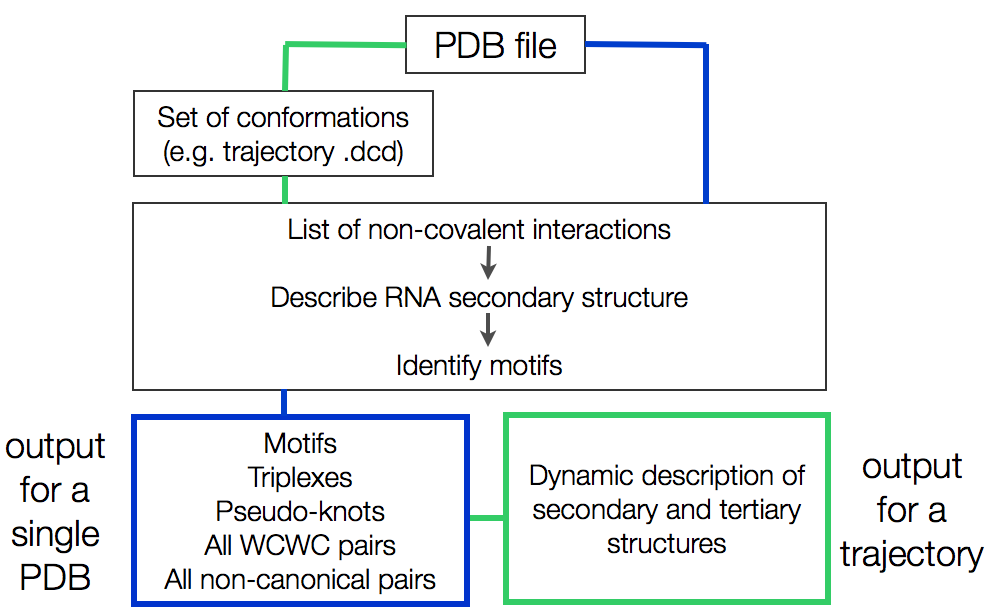
\includegraphics[scale=0.4]{./pictures/workflow.png}
\caption{Main function implements the analysis of a single frame. In the case of a trajectory, the function reads-in the list of nucleotides from a given PDB and then refreshes the atom coordinates while reading the next frame. Additionally, the script splits the trajectory between CPUs and runs separate processes, what  accelerates the calculations.}
\label{ProgramScheme}
\end{figure}

\subsection{Loading the DNA or RNA conformations}
The script uploading structures is written in {\tt Python} programming language (\url{http://python.org}). Its modular structure enables applying it in various programming contexts. Reading the PDB file is implemented by BioPython package (\url{http://biopython.org/wiki/Main_Page}), providing a complete objective structure for dealing with PDBs. The basic object is an atom that apart from the name and number is described with spatial coordinates. A molecule consists of residues that have such attributes as a name, a number and list of atoms. This allows fast and easy access to the nucleotides, atoms and their coordinates.

\section{Running MINT}
Go to the \texttt{MINT} directory and type:
\begin{verbatim}
python MINT.py CONFIG.MINT
\end{verbatim}
and the program will perform a short run for the \texttt{example.pdb} and \texttt{example.dcd}, present in the \texttt{MINT/example/} folder (for details see section \ref{Example_sec}), with all parameters set to their default values. If any error appears check whether you are using {\tt python 2.7} and have all the required packages installed (listed in Section \ref{external_pack}).

MINT uses a simple text configuration file, which specifies input parameters. Each line in the configuration file consists of a keyword identifying the parameter and a value to be used for this parameter. Comments are denoted by the \texttt{\#} character. The syntax is:
\begin{verbatim}
keyword:option # comment
\end{verbatim}

The \texttt{CONFIG.MINT} configuration file, provided in the MINT package contains default configuration. 

\subsection{Analysing the DNA versus RNA structures}
{\tt MINT} contains necessary parameters for analysing both DNA and RNA molecules. {\tt MINT} distinguishes the DNA molecules by the names of the residues in the input PDB file, it expects the DNA nucleotides to be named: Adenine: DA, Guanine: DG, Cytosine: DC, Thymine: DT. Other nucleotides will be treated as RNA or derivatives. 

\subsection{Parameters specified in the \texttt{CONFIG.MINT} configuration file}
\begin{itemize}
\item \texttt{SingleOrTraj} -- [Single/Traj] determines whether a trajectory or a single structure will be analyzed. In the Single mode, only the conformation from the PDB file ) \texttt{file\_name} parameter) will be analyzed. In the Traj mode conformations from \texttt{file\_dcd} file will be analyzed. 
\item \texttt{file\_name} -- [file name] input PDB file containing nucleic acid structure. The file is required in both Single or Traj modes.
\item \texttt{file\_dcd} -- [file name] input file containing multiple conformations, trajectory for the Traj mode. The supported trajectory formats \texttt{are .dcd .xyz .trr .crd} as in the \texttt{MDAnalysis} package.  
\item \texttt{chains\_names} -- [list] the list of chain ids to be analyzed. If left empty, the analysis will be performed for all chains. \textbf{Note,} that for analysis all provided chains are treated as a single chain.
\item \texttt{first\_frame} -- [int] the number of the first frame to be analyzed from the trajectory file. {\bf Note,} that numbering in python starts from 0.
\item \texttt{last\_frame} -- [int] the number of the last frame [int/-1] to be analyzed in the trajectory, if set to -1 the program replaces it with the number of the last frame.
\item \texttt{cutoff} -- [\AA] the cutoff for the distance measured between the C1' carbons of every nucleotide. For distances larger than \texttt{cutoff} the program does not search for hydrogen bonds. Default is \texttt{20}.
\item \texttt{cutoff\_stacking} -- [\AA] the cutoff for the distance  measured between the the centers of mass of every nucleobase. For distances larger than \texttt{cutoff\_stacking} the program does not search for the stacking interaction. Default is \texttt{10.5}.
\item \texttt{vdw\_cutoff\_stacking} --  [kcal/mol] the maximal value of the Van der Waals (VdW) energy for the stacking interaction. If the VdW energy between two nucleobases is smaller than the given \texttt{vdw\_cutoff\_stacking} parameter, the stacking interaction is detected. Default value: \texttt{-0.5}.
\item \texttt{OP\_stacking\_distance\_cutoff} -- [\AA]  the maximal distance between a backbone phosphate group and a nucleobase center of mass for the calculation of the anion-$\pi$ interaction. If measured distance is lower than given \texttt{OP\_stacking\_distance\_cutoff} parameter the anion-$\pi$ interaction is detected. Default is \texttt{4.5}.
\item \texttt{h\_bond\_atom} -- [donor/hydrogen] indicates whether the hydrogen bond distance should be computed between a \textbf{donor} and acceptor or a \textbf{hydrogen} and acceptor. Default is \texttt{donor} 
\item \texttt{h\_bond\_l} -- [\AA] the maximal length  of the hydrogen bond. Default value of {\tt 4} was set in accord with \texttt{h\_bond\_atom:donor}.
\item \texttt{h\_bond\_angle}  -- [degrees] the minimal angle of the hydrogen bond. Default is {\tt 140}.
\item {\tt vmd} -- [0/1] the binary parameter working only in {\tt SingleOrTraj:Single} mode. If 1 a {\tt VMD} application will be opened and the input structure coloured by secondary structures. This is possible only if {\tt VMD} is properly installed and added to PATH (one can rub it with {\tt vmd} command). Step-by-step procedure is detailed in the \ref{VMD} subsection.
\item \texttt{table\_nucleotides} -- [file name] the {\tt .csv} file determining the hydrogen donors, acceptors and nucleotide edges for every nucleotide. By editing this file, one can remove certain interactions from the analysis or define new types of interactions. Default file \texttt{nucleotides\_modified.csv} is stored in the \texttt{MINT/data/} folder.
\item \texttt{table\_charges}  -- [file name] the \texttt{.csv} file listing the partial charges, Van der Waals radii and depths of the Lennard-Jones potential for atoms in nucleotides. These parameters are given for two force fields: AMBER and CHARMM, but there is also a column MY\_OWN for the user to put other parameters if needed. {\color{red} odnosniki do pol silowych zaraz po slowach AMBER i CHARMM}
Default file \texttt{./data/charges\_and\_VDW\_modified.csv} is stored in the \texttt{MINT/data/} folder.
\item \texttt{list\_of\_modified\_nucs} -- the two-column text file with the list of modified RNA nucleotides present in the RNA structures deposited in the PDB database (as of July 2014). Each row contains the residue name used for the modified nucleotide and a single-letter code (a, g, c, t, u) for the natural nucleotide from which the modification originates. Default \texttt{data/unknown\_modified.fa} is stored in the \texttt{MINT/data/} folder.
\item \texttt{force\_field} --  [AMBER/CHARMM/MY\_OWN] the name of the force field to be used by the program while computing stacking energies.
\item \texttt{margin} -- [0.0 -- 1.0]  the minimal portion of nucleotides that have to be common for both motifs to belong to the same cluster. Default is \texttt{0.8}.
\item \texttt{time\_cutoff} -- [0.0,1.0] the minimal portion of the conformations from the trajectory file in which the motifs must be present in, in order to be incorporated into the cluster analysis. Default is \texttt{0.02}.
\item \texttt{max\_memory\_GB} -- [GB] the maximal memory the single thread is allowed to use at one time. Default is \texttt{1.5}.
\item \texttt{threads} -- [int] the number of CPUs to be used while analyzing  the trajectory. Default is~\texttt{1}.
\item \texttt{only\_analysis} -- [True/False] if True, the program instead of running the whole analysis, reads in the previously performed analyses, performs computations only for the missing frames and creates output files. You can turn on this parameter if your computations were disturbed for some reason. In this mode {\tt MINT} uses only one CPU. Default is {\tt False}.
\item \texttt{pdb\_list} -- [file name] if not empty, MINT will read in the list of PDB ids (a file with a PDB ids put in a column -- one per row), download the structures from the PDB database, unpack, protonate using the {\tt reduce} program~\cite{Word1999a} and perform the analysis in a single frame mode. Every analysis will be automatically located in a separate directory.
\end{itemize}

\subsection{Example} \label{Example_sec}
The {\tt example} directory of {\tt MINT} contains the following \textbf{inputs}:
\begin{itemize}
\item \texttt{example.pdb}  -- a .pdb file with the atomic structure of the RNA molecule. One will benefit from the program mostly by analyzing RNA structures with complex secondary and tertiary structures.
\item \texttt{example.dcd}  -- a trajectory file containing ten frames from molecular dynamics simulations performed with NAMD \cite{Phillips2005} and using the CHARMM force field.
\end{itemize}

and \textbf{outputs}:
\begin{itemize}
\item Structure description (see section \ref{OutputFiles} for details):
\begin{itemize}
\item example\_description			
\item example.pdb\_MINT.xls or example.dcd\_MINT.xls (depends on the running mode)
\item example\_nucleotides\_eval.csv
\item example\_pairs\_in\_time.csv
\item example\_helices\_in\_time.csv
\item example\_motifs\_in\_time.csv
\item example\_average\_motifs.csv				
\item example\_motifs\_clusters.csv
\item example\_stacking\_in\_time.csv
\item example\_ion\_pi\_in\_time.csv
\item example\_dot\_bracket.txt
\end{itemize}
\item Visualization  (see section \ref{Visualization} for details):
\begin{itemize}
\item exampleRNAStructML.xml		
\item example\_2D.pdb				
\item example\_3D.pdb				
\item example\_VDW.pdb				
\item example\_stacking\_sum.pdb
\item example\_coulomb.pdb			
\item example\_WC-WC.png
\item example\_3D.png				
\item example\_stacking-VDW.png
\item example\_stacking-sum.pdb
\item example\_stacking-coulomb.png
\item vmd\_run.tcl
\end{itemize}
\end{itemize}

All the examples provided in this manual are derived from above files.

\subsection{Output files}\label{OutputFiles}
The output files describe nucleotides in a way that allows them to be unambiguously identified. We use the representation containing a chain name, a residue name and number. For example: the \texttt{N|GUA:521} represents the residue number 521 from the chain N, with the name GUA. The values posted in the \texttt{chain name|residue name:residue number} code are derived from the input PDB file.

{\tt MINT} generates multiple files both in the single frame analysis mode and in the trajectory mode. Names of the generated files begin with the \texttt{file\_name} for the single frame mode and both \texttt{file\_name} and \texttt{file\_dcd} for the trajectory mode. They are all stored in the directory where the input files are placed.\\

\noindent
Output files:
\begin{itemize}
\item \texttt{\_description} -- contains a complete description of the structure for every frame. The exemplary description is shown in the end of this manual. The single frame description contains a complete list of used parameters, helices, motifs, triplexes, pseudo-knots. One can also find a list of both canonical and non-canonical interactions, with the exact parameters of hydrogen bonds and stacking interactions. Additionally, there is a  dot-bracket representation of the secondary structure that can be used for visualization or energy computation. The frames are separated by the headers: \texttt{frame number}.

\item \texttt{\_MINT.xls} -- a complete .xls file collecting all of the below .csv files. For every .csv file a separate sheet is created. 

\item \texttt{\_pairs\_in\_time.csv} --  a .csv file containing all nucleobase pairs that appeared during the trajectory. The file contains the following columns: \texttt{number of first nuc}, 	\texttt{pair\_nucleotides} (the numbering of paired nucleotides), \texttt{pair type} (e.g. WC) , \texttt{pair configuration} (\textit{cis} or \textit{trans}), \texttt{vmd}, \texttt{percentage of frames a pair was present}, \texttt{frame numbers in which a pair was present}, the exemplary data record is shown below:
{\color{red} czy mozna i w outputach, przykladach ponizej i w manualu dac \texttt{frame numbers in which a pair was present}, zeby bylo konsystentnie oraz \texttt{percentage of frames a pair was present}. W tabelce sa procenty, w opisach liczba klatek, to nie jest uporzadkowane moim zdaniem, to co w tabelce musi dokladnie odpowiadac temu co w tekscie i w outputach. Jesli w przykladzie mamy 10 klatek i mamy 50 procent w ktorych jest para to dlaczego jest 0 albo co to oznacza 0->1? Uporzadkujcie to prosze. To dotyczy wielu tabel ponizej. Dodatkowo jesli sie nie da sformatowac, zeby tabelka byla od razu po dwukropku jak jest below albo the following to trzeba je ponumerowac i dodac captions.}

\begin{table}[h!]
\begin{tabular}
{ | >{\centering} m{1.3cm} | >{\centering} m{2.3cm} | >{\centering} m{3cm}  | >{\centering} m{2.5cm} | >{\centering} m{1.5cm} |>{\centering} m{2.3cm} |>{\centering} m{2cm} |}  \hline 
number of first nuc &	 pair \_nucleotides	& pair type	&  pair configuration	&  vmd	  & number of frames a pair was present & frames in which a pair was present \tabularnewline \hline \hline
515&	N$|$GUA:515/ N$|$CYT:536 &	WC/WC	 & Cis	&  resid 515 536	& 100,00\%	 & $ 0\rightarrow 1$  \tabularnewline \hline
516&	N$|$URA:516/ N$|$CYT:519&	WC/Hoogsteen	& Trans & resid 516 533	& 50,00\% &	 $ 0$  \tabularnewline \hline
522&	N$|$CYT:522/ N$|$GUA:527&	WC/WC &	 Cis	& resid 522 527 &	100,00\%	& $ 0\rightarrow 1 $ \tabularnewline \hline
\end{tabular}
\end{table}

\item csv file for every type of the secondary structure. {\tt .csv} files are easy to manipulate and can be opened with any popular spread-sheet applications. All of the files:  
\begin{itemize}
\item \texttt{\_helices\_in\_time.csv},
\item  \texttt{\_motifs\_in\_time.csv}, 
\item \texttt{\_pseudo\_in\_time.csv},
\item \texttt{\_triplex\_in\_time.csv},
\end{itemize}
contain five  columns: 
\begin{itemize}
\item \texttt{motif\_topology} - absent in the  \texttt{\_helices\_in\_time.csv}, for explanation see \ref{RNA_motifs},
\item \texttt{motif\_nucleotides}  - nucleotides creating the motif,
\item \texttt{vmd} - ready to paste into the VMD residual identifiers,
\item \texttt{percentage of the frames a motif was present},
\item \texttt{frame numbers in which a motif was present}.
\end{itemize}  
The example can be found in the table below (residues are removed just for presentation): {\color{red} jakie residues sa removed, nie rozumiem, sa w tabelce?}
\begin{table}[h!]
\begin{tabular}
{ | >{\centering} m{1.5cm} | >{\centering} m{5cm} | >{\centering} m{4.5cm}  | >{\centering} m{3.3cm} | >{\centering} m{2.3cm} |}  \hline
motif \_topology	& motif\_nucleotides &vmd&percentage of frames motif was present& frames when motif was present  \tabularnewline \hline \hline
7-5	 & N$|$GUA:515-N$|$CYT:536 ... N$|$URA:516-N$|$GUA:515	 & chain N and resid 515 536 .. 516 515 & 	100,00\%	 & $0 \rightarrow 1 $ \tabularnewline \hline
4 & N$|$CYT:522-N$|$GUA:527 ... N$|$ADE:523-N$|$CYT:522& chain N and resid 522 527 .. 523 522 & 100,00\%	& $ 0\rightarrow  1 $ \tabularnewline \hline
0-6 &	N$|$CYT:504-N$|$GUA:541 ... N$|$GUA:505-N$|$CYT:504	& chain N and resid 504 541 .. 505 504  &	100,00\%	& $ 0\rightarrow 1$ \tabularnewline \hline
\end{tabular}
\end{table}

\item \texttt{\_stacking\_in\_time.csv} -- a .csv file containing all nucleotide pairs recognized as stacked. The file contains the following columns: \texttt{number\_of\_the\_first}, \texttt{stacking\_bases}, \texttt{avg\_coulomb\_energy} (the Coulomb interaction energy in kcal/mol),	\texttt{avg\_vdw\_energy} (the VDW interaction energy in kcal/mol), \texttt{avg\_sum\_energy} (sum of the VDW and Coulomb interactions for the recognized pair in kcal/mol), 
\texttt{vmd}, 
\texttt{percentage\_of\_frames\_pair was present},	
\texttt{frames\_when pairs\_was\_present}. 
The \texttt{\_ion\_pi\_in\_time.csv} file describes ion-$\pi$ interactions and is constructed analogously. Example of the \texttt{\_stacking\_in\_time.csv} file:
{\color{red} nadal nie rozumiem co to sa za strzalki w ostatniej kolumnie bo moim zdaniem nie bylo to wczesniej wyjasnione. Jesli w kolumnie sa procenty i jest 1 albo 0.25 to jakie sa jednostki czy procent?}
\begin{table}[h!]
\centering
\begin{tabular}
{ | >{\centering} m{2cm} | >{\centering} m{2cm} | >{\centering} m{2.1cm}  | >{\centering} m{1.8cm} |>{\centering} m{1.7cm}| >{\centering} m{2cm}|>{\centering} m{2.2cm}| >{\centering} m{2cm}| } \hline 

 number\_of\_ the\_first	&  stacking\_ bases	&  avg\_coulomb \_energy 
&	avg\_vdw \_energy	&  avg\_sum \_energy	& vdw  & percentage of frames a pair was present	& frames in which a pair was present
\tabularnewline \hline \hline

509	& N$|$ADE:509 \_N$|$ADE:510&	26.18&	-27.4	&-1.22&	chain N and resid  509 510 &	1 &	 $0 \rightarrow 4$
\tabularnewline \hline

501	& N$|$CYT:501 \_N$|$CYT:545&	8.6&	-5.81	&2.78&	chain N and resid  501 545  &	1 &	 $0 \rightarrow 4$
\tabularnewline \hline

502	& N$|$ADE:502 \_N$|$GUA:544&	2.04&	-22.92	&-20.87&	chain N and resid  502 544   &	0.25 &	 2
 \tabularnewline \hline
\end{tabular}
\end{table}
{\color{red} skrot na van der Waals jest raz VdW a raz Vdw, poprosze, zeby nie bylo niechlujnie i jak raz oznaczycie skrot to zeby on i w tabelkach, outputach i w tekscie byl taki sam}

\item \texttt{\_nucleotides\_eval.csv} -- thie .csv file contains the physical description of single nucleotides. The \texttt{2d-hbonds} column corresponds to the number of hydrogen bonds created by a nucleotide in the WC pairs, analogously \texttt{3d-hbonds} is the number of hydrogen bonds in non-WC pairs. {\color{red} czy mozna sie tu odniesc do edges i to uscislic?} The \texttt{Coulomb}, \texttt{Vdw} and the \texttt{sum} columns contain values of stacking energy interactions per nucleotide. These interactions are originally computed for pairs -- a single nucleotide is described with the sum of all interactions of a given kind. {\color{red} Therefore, if one is looking on how much the nucleotide is fisted this is a good measurement, nie rozumiem tego zdania} but while looking at the several nucleotides keep in mind not to incorporate energies more than once. In the case of the trajectory these are average numbers: 

\begin{table}[h!]
\centering
\begin{tabular}
{ | >{\centering} m{2cm} | >{\centering} m{1.3cm} | >{\centering} m{1.9cm}  | >{\centering} m{1.9cm} |>{\centering} m{1.8cm}| >{\centering} m{1.3cm}| >{\centering} m{1.5cm}| >{\centering} m{3.9cm}|} \hline 
nuc	& num	& 2d-hbonds &	3d-hbonds	& Coulomb	& Vdw	& sum & vmd \tabularnewline \hline \hline
N$|$ADE:502 & 502 &	2,00 &	0,00	& 1,57 &	-15,74 &	-14,18 & chain N and resid  502 \tabularnewline \hline
N$|$GUA:517 & 517 &	0,00 &	0,50	& 5,73	&-10,65 &	-4,92& chain N and resid  517  \tabularnewline \hline
N$|$GUA:515 & 515 &	3,00 &	0,00 &	2,19 &	-20,83 &	-18,64& chain N and resid  515  \tabularnewline \hline
\end{tabular}
\end{table}

\item \texttt{\_motifs\_clusters.csv} -- a .csv file with clusters of motifs; the file contains all motifs assigned to clusters, and overall percentage of the frames the given motif was present (occurrence) and the frame numbers. Frames and clusters are numbered starting from zero:
{\color{red} znow jesli procent to do 100 procent, nie ma tez opisu kolumn ani w tekscie ani w tabelce}
\begin{table}[h!]
\centering
\begin{tabular}
{ | >{\centering} m{1.7cm} | >{\centering} m{0.6cm} | >{\centering} m{5.0cm}  | >{\centering} m{5.0cm} |>{\centering} m{1cm}| >{\centering} m{2.3cm}|} \hline 
cluster 0 & 4-0 & A520-A533-...- G521-A520- &chain N and resid 520 533 ... 521 520 &0.3& $ 3\rightarrow 4 9 $\tabularnewline \hline
cluster 0 & 7-5 & G515-...-U516-G515- &chain N and resid 515 536 ... 516 515 &0.7& $ 0\rightarrow 2 5\rightarrow 8 $ \tabularnewline \hline
cluster 0 & 2-4 & G515-...-U516-G515- &chain N and resid 515 536 ... 516 515 &0.3& $ 3\rightarrow 4 9 $\tabularnewline \hline
cluster 1 & 4 & C522-G527-...-A523-C522- &chain N and resid 522 527... 523 522 &1.0& $ 0\rightarrow 9 $\tabularnewline \hline
cluster 2 & 0-6 & C504-G541-...-G505-C504- &chain N and resid 504 541 ... 505 504 &1.0& $ 0 \rightarrow 9 $ \tabularnewline \hline
\end{tabular}
\end{table}

\newpage
\item \texttt{\_average\_motifs.csv} - a .csv file representing the list of average motifs, derived from the cluster list and a nucleotide characteristics list. The vector described as {\tt 2D} contains the average numbers of hydrogen bonds created by the  nucleotides in the WC-WC interactions, a \texttt{3D} vector is analogous but for non-WC interactions:
\begin{table}[h!]
\centering
\begin{tabular}
{ | >{\centering} m{0.4cm} | >{\centering} m{0.7cm} | >{\centering} m{5.5cm}  | >{\centering} m{3.5cm} |>{\centering} m{1cm}|>{\centering} m{2cm}|} \hline 
1&4&C522-G527-...-A523-C522-& resid 522 ... 522 & 1.0& $ 0 \rightarrow 9 $  \tabularnewline \hline
&2D&3.0  3.0  2.8 ...  0.0  3.0 &&& \tabularnewline \hline
&3D&0.0  3.0  0.8 ...  2.1  0.0 && &\tabularnewline \hline
2&0-6&C504-G541-...-G505-C504-&resid 504 ... 504 &1.0&$ 0 \rightarrow 9 $  \tabularnewline \hline
&2D&2.9  2.9  ...  2.8  2.9 &&& \tabularnewline \hline
&3D&0.0  0.0  ...  0.0  0.0 &&&\tabularnewline \hline
\end{tabular}
\end{table}
\item \_dot\_bracket.txt - a simple text file created only in the \texttt{Trajectory} mode. Sequential lines contain the dot-bracket representation of the secondary structure for corresponding frames of the trajectory. This file enables analyzing the evolution of the secondary structure in external tools:
\begin{verbatim}
(((((......(((((.....((....)).......))))))))))
(((((......(((((.....((....)).......))))))))))
(((((......(((((....(((....))....)..))))))))))
(((((......(((((....(((....))....)..))))))))))
(((((......(((((....(((....))....)..))))))))))
\end{verbatim}

\item Figures of the average secondary structure coloured by the values of computed parameters, generated using the  {\tt VARNA} \cite{Blin2009} program. The sequence is retrieved directly from an input PDB file. The secondary structure is computed from the list of WC base pairs -- in the case of the single frame from an input PDB file and in the case of the trajectory from the list of the most represented WC-WC pairs. Figure \ref{varna} presents 5 images visualizing:
\begin{itemize}
\item 2D: Number of WC hydrogen bonds .
\item 3D: Number of non-WC hydrogen bonds.
\item Stacking Coulomb: Coulomb term of Stacking energy in kcal/mol. 
\item Stacking VDW: VDW term of Stacking energy in kcal/mol.
\item Stacking Sum: Sum of the Coulomb and Van der Waals interactions in kcal/mol. 
\end{itemize}

In case of energy terms (Coulomb and Van der Waals) the scale of colors is reversed so the red nucleotides are the ones that are influenced by the strongest hydrogen bonding and stacking interactions.  

\begin{figure}[h!]
\centering
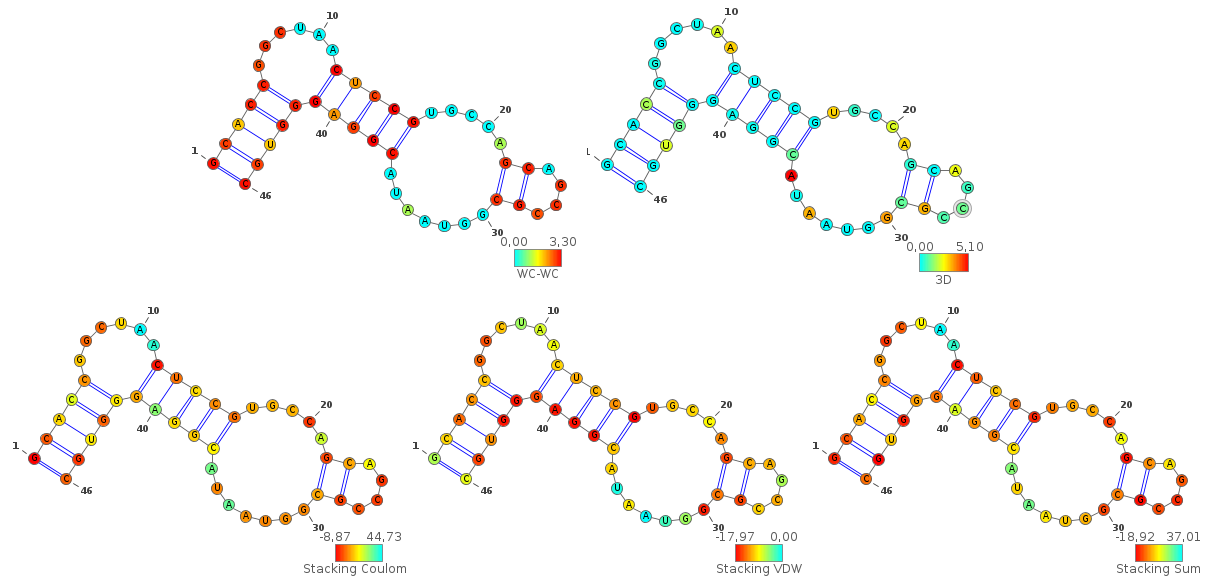
\includegraphics[scale=0.6]{./pictures/varna3.png}
\caption{Figures with average secondary structure coloured by the values of computed parameters, generated by MINT and displayed with the VARNA \cite{Blin2009} program.}
\label{varna}
\end{figure}


\newpage

\item Files needed for visualization using external tools (see Section \ref{Visualization} for details):
\begin{itemize}
\item \texttt{\_RNAStructML.xml} 
\item \texttt{\_2D.pdb}
\item \texttt{\_3D.pdb}
\item \texttt{\_coulomb.pdb}
\item \texttt{\_VDW.pdb}
\item \texttt{\_stacking\_sum.pdb}
\item \texttt{vmd\_run.tcl}
\end{itemize}
\end{itemize}

Detailed description of the visualization procedures can be found below.


\section{Methodology for calculating physicochemical features}
\subsection{Hydrogen bonding}
\label{Hbond-section}
A hydrogen bond is a basic interaction responsible for creating the secondary and tertiary structures of nucleic acids. A typical definition of a hydrogen bond pertains to a non-covalent interaction when a hydrogen atom is placed close to its acceptor.

Both the distance and the angle (Figure \ref{hbond}) depend on the characteristics of the donor and acceptor. Theory states that all hydrogen bonds are almost linear (around $175^\circ$) \cite{Guerra2000}. For biological molecules the hydrogen bond distance should be typically between 2,80 and 3,06 \AA\ between a donor and acceptor, which gives 1,60 and 1,80 \AA\ between an acceptor and hydrogen. The user can decide which distance will be measured by {\tt MINT} using the \texttt{h\_bond\_atom} parameter.
Other user defined parameters are: the minimal angle and the maximal length of a hydrogen bond. The default values of the \texttt{h\_bond distance} (4 \AA) and the \texttt{h\_bond\_angle} ($140^\circ$) are consistent with the distance calculated between donor and acceptor atoms. 

\begin{figure}[h!]
\centering
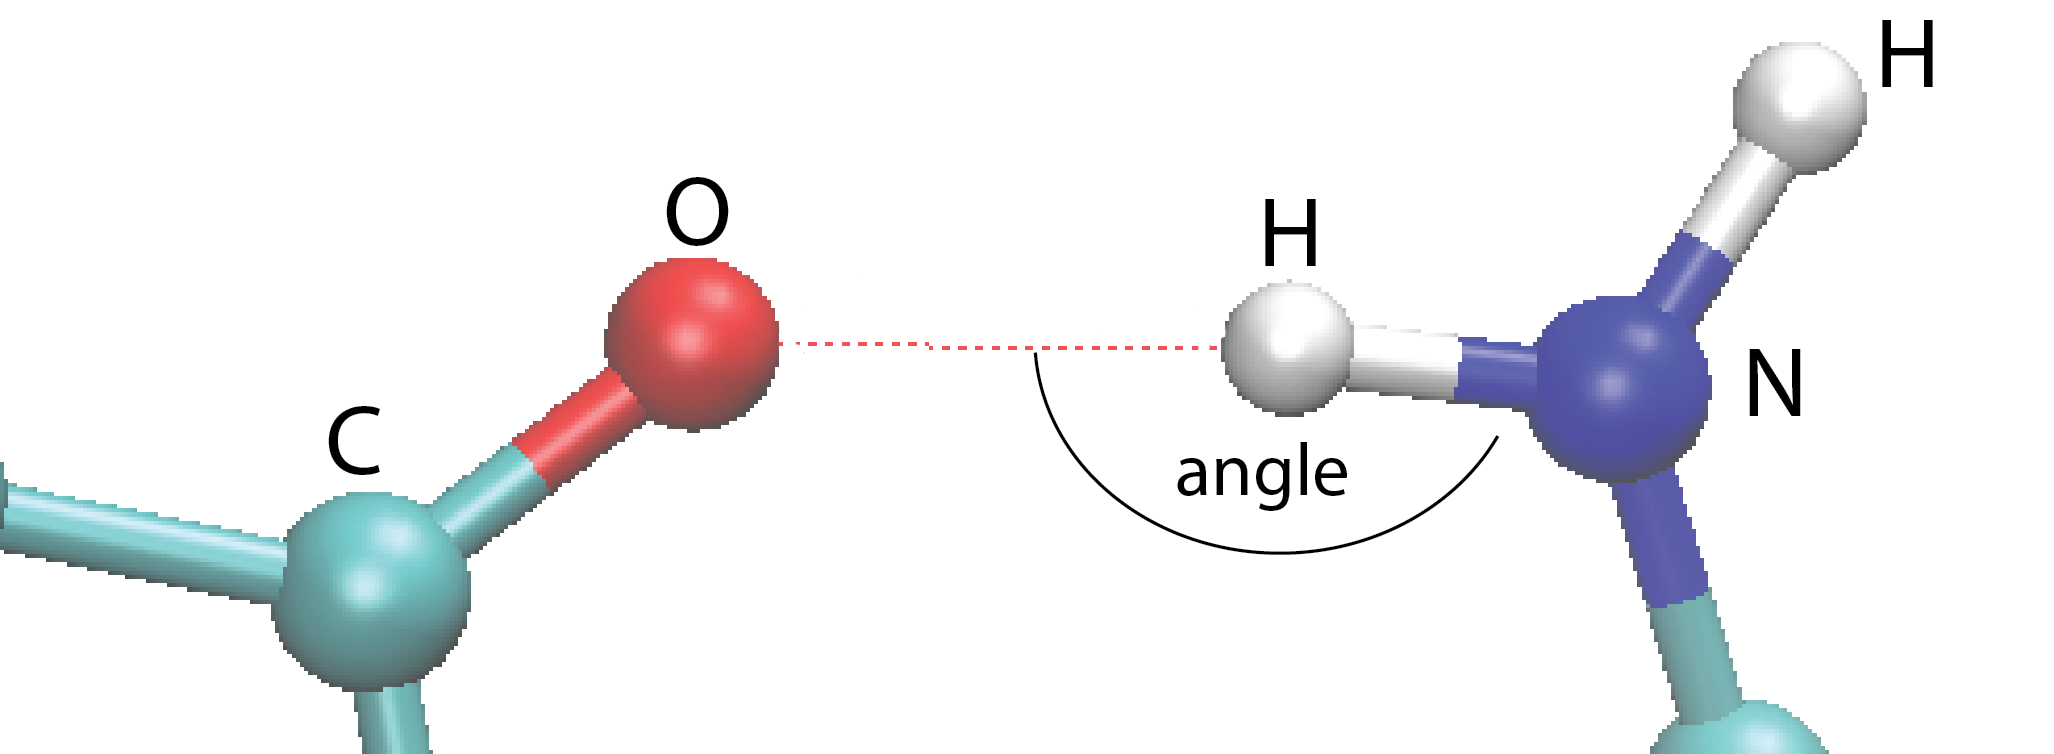
\includegraphics[width = 10cm]{./pictures/hydrogen_bond_2.png}
\caption{The scheme of the hydrogen bond with the nitrogen atom as a donor and the oxygen atom as an acceptor.}
\label{hbond}
\end{figure}

\subsection{Donors and acceptors}
\label{donrsandacceptors}
To analyze the structures we have defined a list of possible acceptors and donors for all nucleotides of RNA and DNA. Following the classification by Leontis and Westhof \cite{Leontis2002} the acceptors and donors are assigned to the edges of the nucleotide, as shown in Figure \ref{Edges}. This classification is stored in the {\tt table\_nucleotides} .csv file and may be edited by the user. 

{\tt MINT} determines the interacting edges of every pair of nucleotides. Several atoms are situated in the corners of the nucleotides and participate in more than one edge. In that case, the program first classifies all the remaining bonds and chooses the prevailing edge. If there is only one hydrogen bond, both edge names are returned. 

\begin{figure}[h!]
\centering
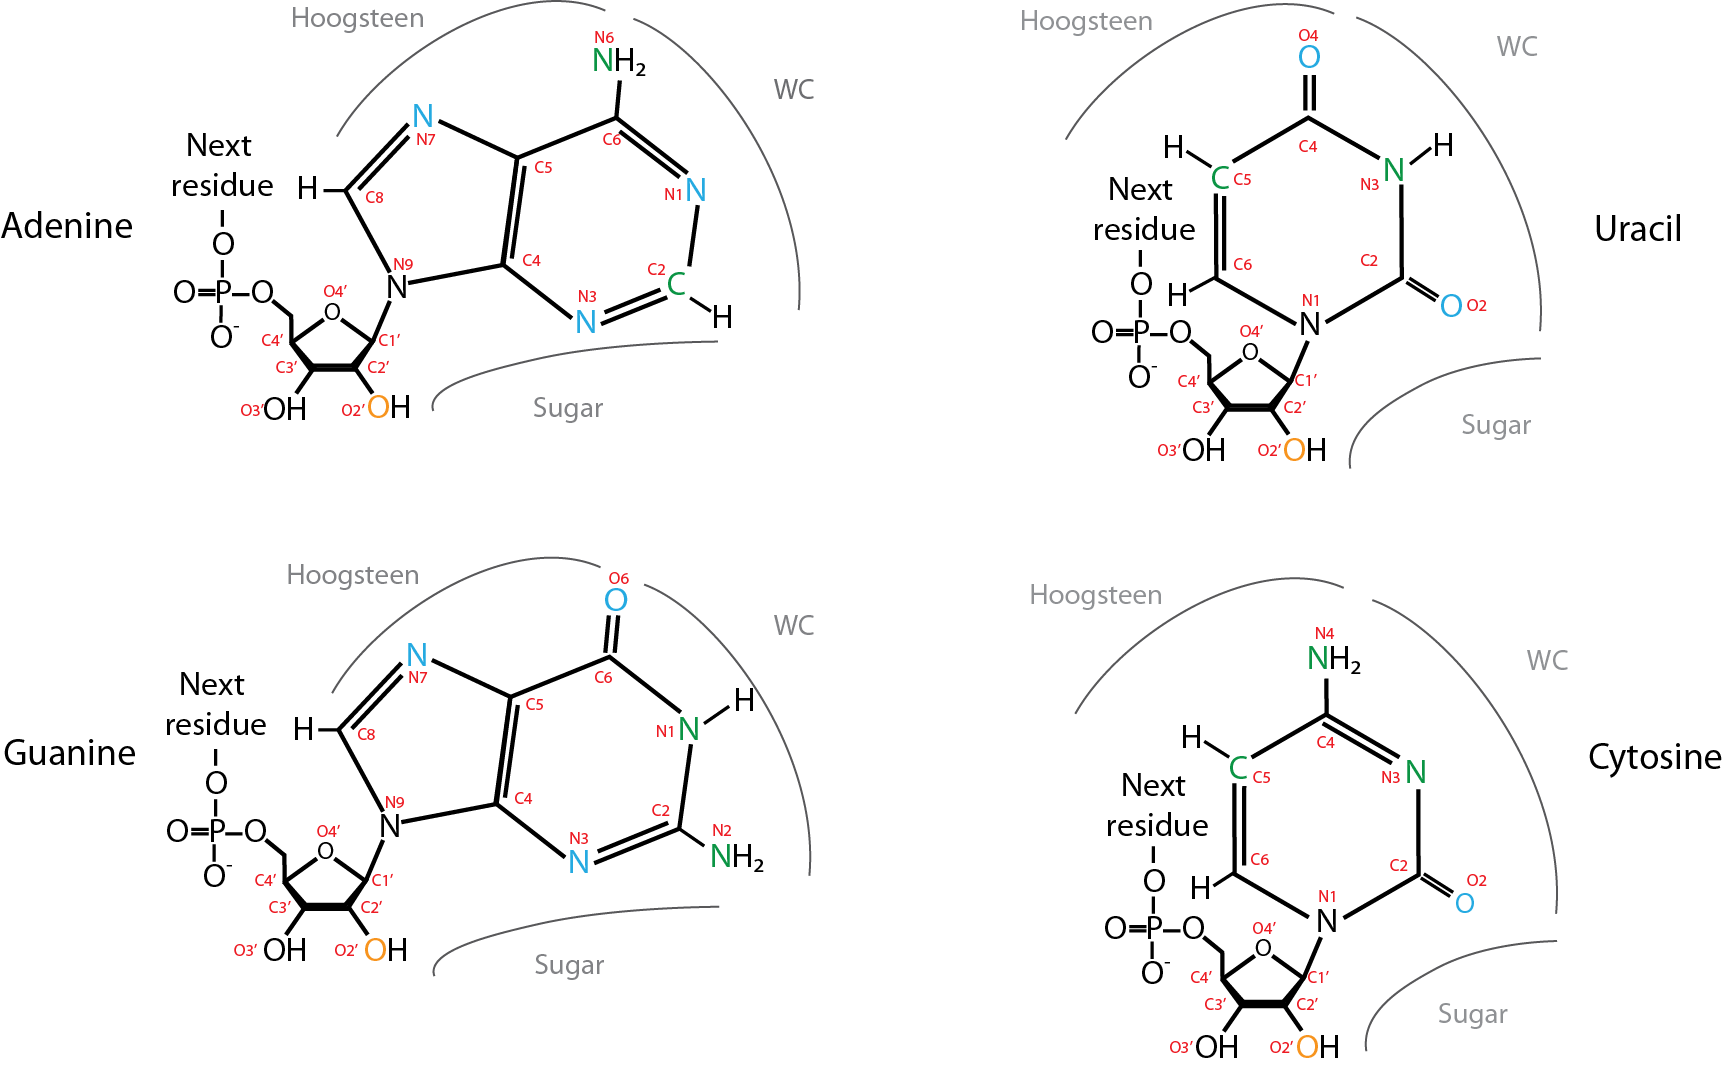
\includegraphics[width = 14cm]{./pictures/donors_acceptors_nucleotides.png}
\caption{Nucleotides with selected edges, donors (green) and acceptors (blue). WC corresponds to WC edge.  \cite{Lescoute2006}. {\color{red} jest literowka w Next residue jest Nexit!}}
\label{Edges}
\end{figure}

% Pairs
{\tt MINT} checks all the donors against all acceptors in all possible pairs of all nucleotides in the molecule. In order to decrease the computational time, we assume that the partner for a given nucleotide can be found only among its closest neighbors. The exact distance is defined by the user in the {\tt cutoff} parameter. Knowing the atoms creating hydrogen bonds, the program  determines the interacting edges.

\subsection{Modified nucleotides}
Modified nucleotides are functionally important and are found in almost all RNAs, for example, in tRNAs. A few modified nucleotides are presented in Figure \ref{ModifiedNucleotides}. 
\begin{figure}[h!]
\centering
\begin{center}
\subfigure[2MG]{
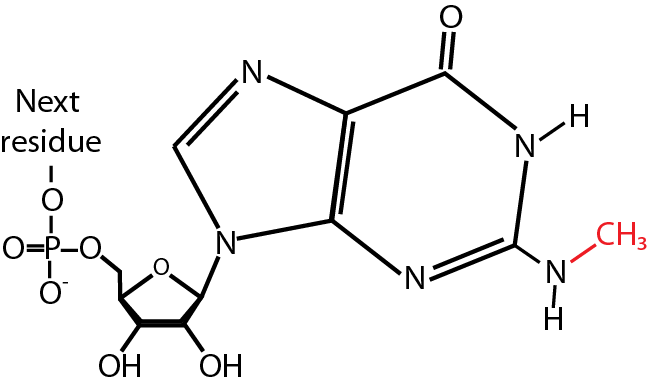
\includegraphics[scale=0.8]{./pictures/modified_1.png}}
\subfigure[OMC]{
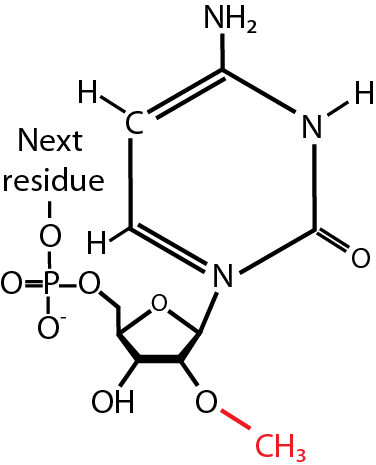
\includegraphics[scale=0.8]{./pictures/modified_2.png}}
\subfigure[YYG]{
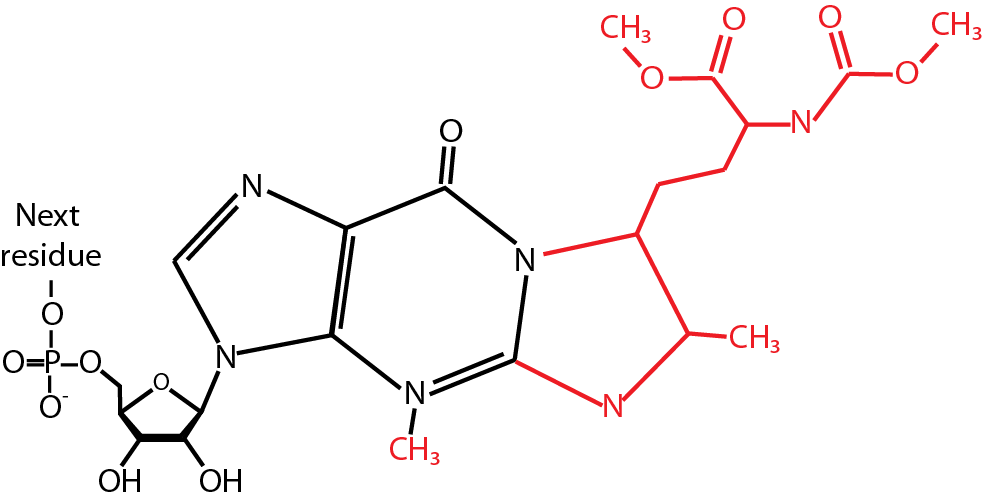
\includegraphics[scale=0.8]{./pictures/modified_3.png}}
\end{center}
\caption{Three out of ten modified nucleotides present in the structure of tRNA (PDB code: 1TTT) along with their PDB names. The atoms that are not present in standard nucleotides are shown in red. {\color{red} znow jest Nexit residue}}
\label{ModifiedNucleotides}
\end{figure}

There are about 600 modified RNA nucleotides in the PDB database, but for most of them there are no force field parameters. With {\tt MINT} we provide the VDW parameters and partial atomic charges for 107 naturally occurring modified nucleotides whose force fields were developed by Aduri et al~\cite{Aduri_2007}. For these nucleotides, we have also assigned their atoms to distinct edges: the WC edge, the Hoogsteen edge, the sugar edge and to the edge termed the modification edge (see Section \ref{donrsandacceptors} for details about the classification of edges). 

An atom in a modified nucleotide, common to the unmodified one, is assigned into the same edge as in the unmodified nucleotide. The addition of no more than one heavy atom to the nitrogenous base is also classified into the same edge as the base atom. The 2'O methyl carbon is assigned to the sugar edge. All other atoms present in the modified nucleotide but not in the original one are assigned to the modification edge.

If {\tt MINT} encounters a modified nucleotide, it looks for its parameters in the {\tt table\_nucleotides}. If parameters are not found, {\tt MINT} uses the \texttt{list\_of\_modified\_nucs} to find the natural ancestor of the modification. Atoms common to the modified and its natural ancestor are assigned analogously as in the original nucleotide, the rest is assigned to the modification edge. If there are no partial charges and VDW parameters, the stacking interaction energy is set to 0.

However, the user can add new modified nucleotides. The force field parameters developed for a modified nucleotide for an MD simulation, can be adopted to the {\tt MINT} parameter format. If you want to add your own modification to the {\tt MINT} parameters: you should edit the {\tt table\_nucleotides} file and add a new row with the name of your residue and appropriate names of atoms in the donor and acceptor columns. Next, you should also modify the \texttt{table\_charges} file. For every atom that should be considered in stacking computation you have to add a row with the name of the residue, charge, VDW radius and well depth parameter. For details see Sections \ref{Hbond-section} and~\ref{stacking-section}.

\subsection{Geometric isomerism of base pairs}
For detected base pairs the geometric isomerism of their glycosidic bonds is computed. The program measures the torsion angle formed by the four atoms (C1', N1 in pyrimidines and C1', N9 in purines) and depending on its value a {\it cis} or {\it trans} conformation is denoted (see Figure \ref{Conf}).

\begin{figure}[h!]
\begin{center}
\subfigure[Cis]{
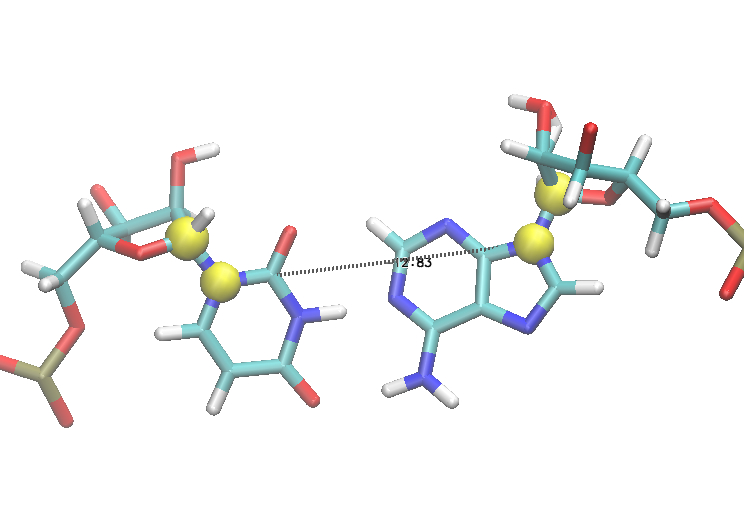
\includegraphics[width=6.5cm]{./pictures/torsion_angle_cis.jpg}}
\subfigure[Trans]{
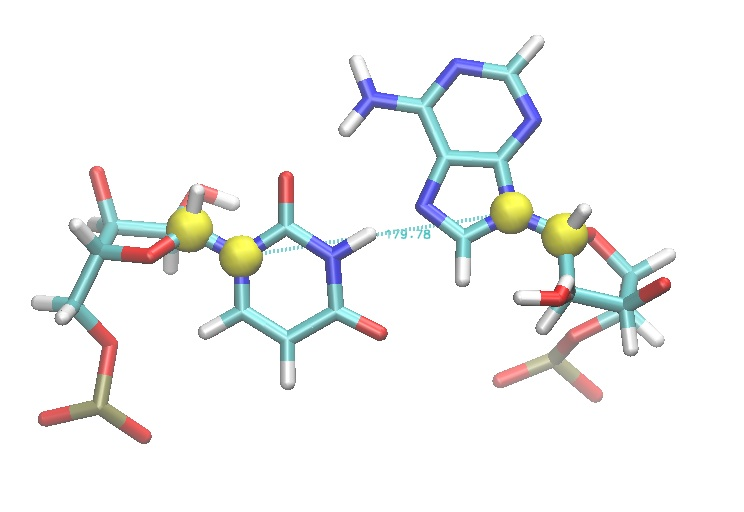
\includegraphics[width=6.5cm]{./pictures/torsion_angle_trans.jpg}}
\end{center}
\caption{Yellow spheres correspond to C1' and N1 atoms in pyrimidines and N9 atoms in purines. The torsion angle created by these four points determines the geometric isomerism of the two nucleotides creating a pair. }
\label{Conf}
\end{figure}

%Stacking interactions
\subsection{Stacking}
\label{stacking-section}
Stacking is an important non-covalent interaction contributing to the stability of both double helix and single stranded structures of nucleic acids \cite{Hobza2008}. For instance, in tRNA only half of the nucleotides form a helix but about 90\% are stabilized by stacking \cite{Bloomfield1999}. 
\begin{figure} [h!]
\begin{center}
\subfigure[]{
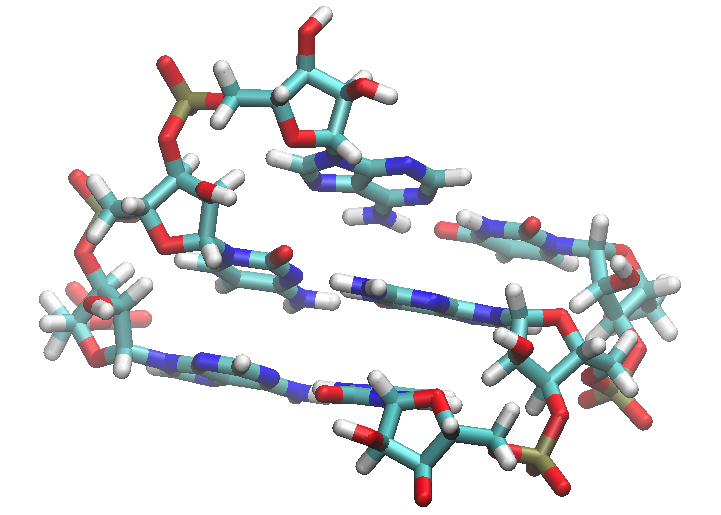
\includegraphics[width=5.0cm]{pictures/stacking1.png}}
\subfigure[]{
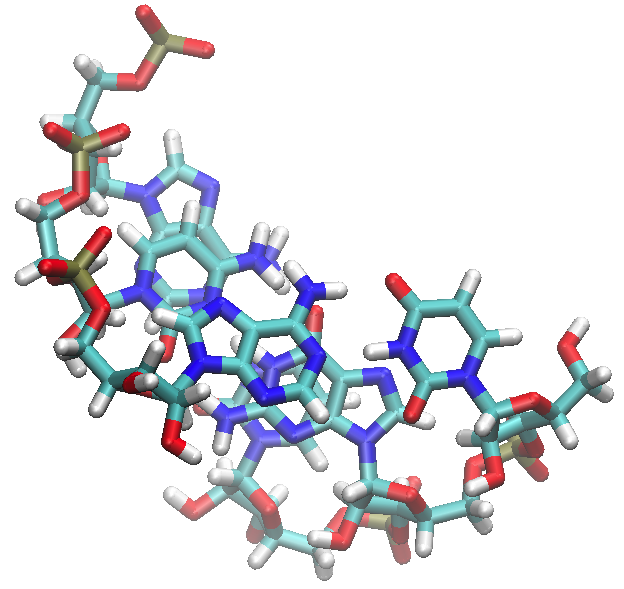
\includegraphics[width=5.0cm]{pictures/stacking2.png}}
\subfigure[]{
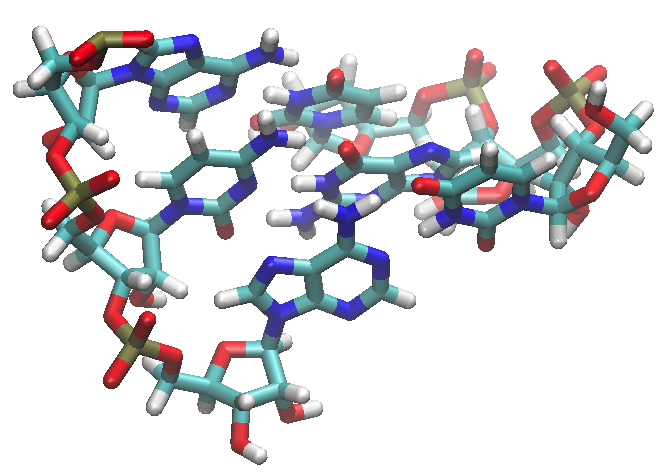
\includegraphics[width=5.0cm]{pictures/stacking3.png}}
\caption{Three-pairs of an RNA helix seen from different angles to expose  stacking between parallel bases.}
\label{StackingHelix}
\end{center}
\end{figure} 
Generally, stacking occurs between aromatic rings so in nucleic acids between the nucleobases. There is a general belief that stacking results from the contact of the electron $\pi$-systems. Stacking also arises from three phenomena: Van der Waals (dipole or induced-dipole attractions), electrostatic and solvation effects. Stacking interactions seem to be more important in folding of nucleic acids than proteins because nucleobases are more polarizable than most amino-acids. 

%In order to measure stacking separately of hydrogen bonding the experiments where conducted with a helix terminated with a single nucleotide. Presence of the unpaired nucleotide  stabilizes the entire helix. Sites are uneven, for DNA the on the $5\prime$ site of the helix is more favorable energetically than the other one, but for RNA the $3\prime$ is \cite{Kool2001}. Experimental studies indicated ability of stacking among natural bases is the strongest between two purines, than purine-pyrimidine and pyrimidine-pyrimidine \cite{Guckian2010}.

Stacking is believed to be represented well in molecular modeling, especially with the Amber atomic charges which are fitted to molecular electrostatic potentials~\cite{Hobza2008}. It was shown that calculations using the empirical potentials consisting of the Lennard-Jones VDW and Coulombic terms with atom-centered point charges reproduced the {\it ab initio} stacking energy over the major portion of the conformational space~\cite{Leszczynski2002}.
\v{S}poner et al. in many studies~\cite{Carter2000,Sponer1997, Base1996, Hobza1995} compared {\it ab initio} energies for about 300 geometries of stacked base dimers with the data obtained using empirical potentials. The agreement between these methods is remarkable, which suggests that calculations based on empirical potentials provide an excellent approximation of the stacking interaction energy between nucleotides. Therefore, MINT calculates the stacking interactions.

We estimate stacking between two bases by calculating the energy of electrostatic ($U_{el}$) and Van der Waals ($U_{VDW}$) interactions applying the equations used in molecular mechanics:
\begin{equation}
U_{el} = k \sum{\frac{q_i q_j}{r_{ij}}}
\end{equation}

\begin{equation}
U_{VDW} = 4 \epsilon_{ij} \sum{ \left[ \frac{1}{4} {\left( \frac{r_0}{r_{ij}} \right) }^{12} - \frac{1}{2} {\left( \frac{r_0}{r_{ij}} \right) }^{6} \right]}
\end{equation}
The sums run over all atom pairs of nucleobases $i$ and $j$, $k$ denotes the Coulomb constant ($k = \frac{1}{4 \Pi \epsilon_0}$), $q$ is the partial atomic charge of the atom, $r_{ij}$ is the distance between the considered atoms, $\epsilon_{ij}$ is the depth of the Lennard-Jones potential well for atoms $i$, $j$ ($\epsilon_{ij} = \sqrt{\epsilon_{ii}\epsilon_{jj}} $) and $r_0$ is the sum of VDW radii of atoms $i$ and $j$. We provide the VDW well depth parameters and partial atomic charges from the Amber~\cite{Wang2000} and Charmm~\cite{Mackerell2000,Foloppe2000} force fields. A set of parameters and charges may be also defined by the user in the file \texttt{table\_charges} file. Only the nucleobases that are closer than the user defined cutoff (\texttt{cutoff\_stacking}) are considered in the stacking calculations. The energy unit obtained from described calculations is $kcal/mol$. 

The electrostatic term, depending on the orientation of base dipole moments, may be attractive or repulsive regardless of the mutual orientation of the bases (parallel or not). While the VDW energy component is almost always favorable regardless of the orientation of bases. Moreover, the shape of nucleotides and the method used for calculating the VDW energy ensure that the lowest VDW energy values are obtained for the parallel orientation of nucleobases (with their largest overlap). This was also the case in our test calculations. Thus we recognize two nucleotides as stacked, if their VDW energy is lower than the \texttt{vdw\_cutoff\_stacking} parameter. The default value of this parameter is $ -0.5 kcal/mol$ which was found by trial and error and seems appropriate for the nonmodified nucleobases.

%\subsection{Anion-$\pi$ contacts} Following recent research on the types of non-covalent contacts in RNA molecules, \texttt{MINT} also analyzes the anion-$\pi$ - contacts and hydrogen bonding interactions, per nucleotides and in pairs \cite{Auffinger2013}. Detection of these interactions is based on the distance between the oxygen atom and the center of the mass of a nucleobase ring. 

\subsection{Ion-$\Pi$ interaction between a nucleobase and phosphate oxygen}
Hydrogen bonds are the most known non-covalent interactions but are not the only one. For example, the cation-$\Pi$ interactions, namely the non-covalent bonding between a monopole (cation) and a quadrupole ($\Pi$ system), play a role in the structure of proteins. A similar interaction was reported for RNA but it was found that nucleic acid aromatic systems prefer to interact with anionic rather than cationic species~\cite{Auffinger2013}. 
{\tt MINT} enables searching for anion-$\Pi$ interactions involving the RNA backbone phosphate groups and nucleobases. An example of such a contact is shown in Figure \ref{stackingPiExamples}.
\begin{figure}[h!]
\begin{center}
\subfigure[]{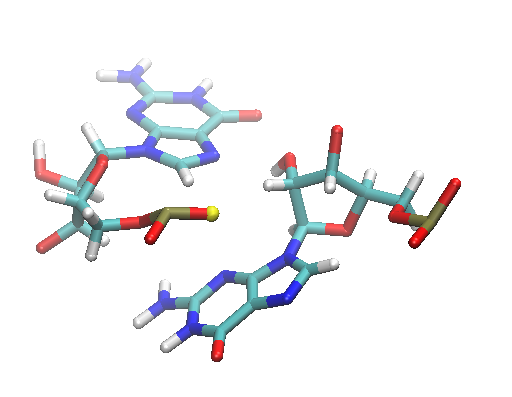
\includegraphics[scale = 0.3]{pictures/stacking_pi_1.png}
\label{stackingPiexample1}}
\subfigure[]{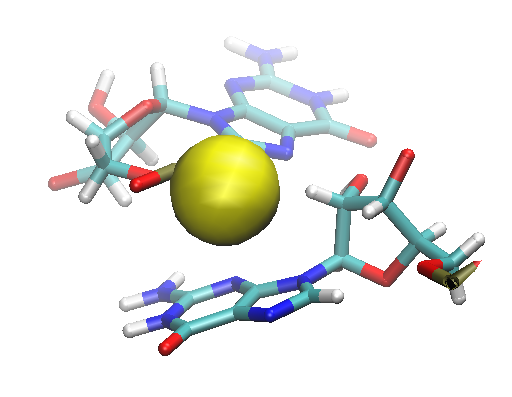
\includegraphics[scale = 0.3]{pictures/stacking_pi_2.png}
\label{stackingPiexample2}}
\subfigure[]{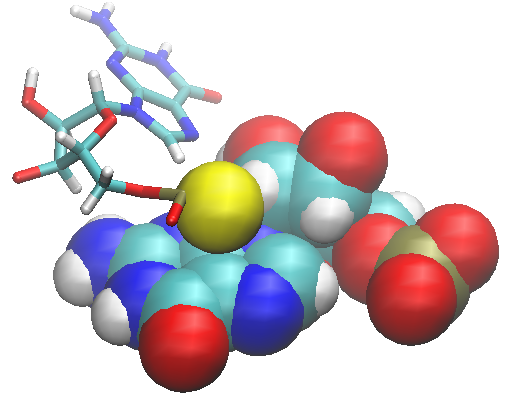
\includegraphics[scale = 0.3]{pictures/stacking_pi_3.png}
\label{stackingPiexample3}}
\caption{Three representations of the oxygen atom (yellow) "stacking" over the guanine base. The yellow sphere in the \label{stackingPiexample1} picture corresponds to the real VDW radius.}
\label{stackingPiExamples}
\end{center}
\end{figure}
The interacting systems are recognized if the distance between a phosphate atom and nucleotide base center of mass is lower than the \texttt{OP\_stacking\_distance\_cutoff} parameter (default distance is $ 5 \AA$). If the ion-$\Pi$ stacking is detected, the energy of interaction between the phosphate atom and nucleobase is calculated in the same way as for the stacking between two nucleobases. 

\subsection{Representation of RNA motifs}
Having all WC pairs, a list-representation of the RNA secondary structure is created. We assume that one nucleotide can have only one WC partner. If the second WC partner is encountered, all three nucleotides are denoted as a triplex. The index of the list represents the nucleotide number and the stored value is the index of its WC partner. The list is easy-interpretable when the arcs connecting the pairs are drawn as  presented in Figure \ref{SecondaryStructureList}. 

\begin{figure}[h!]
\centering
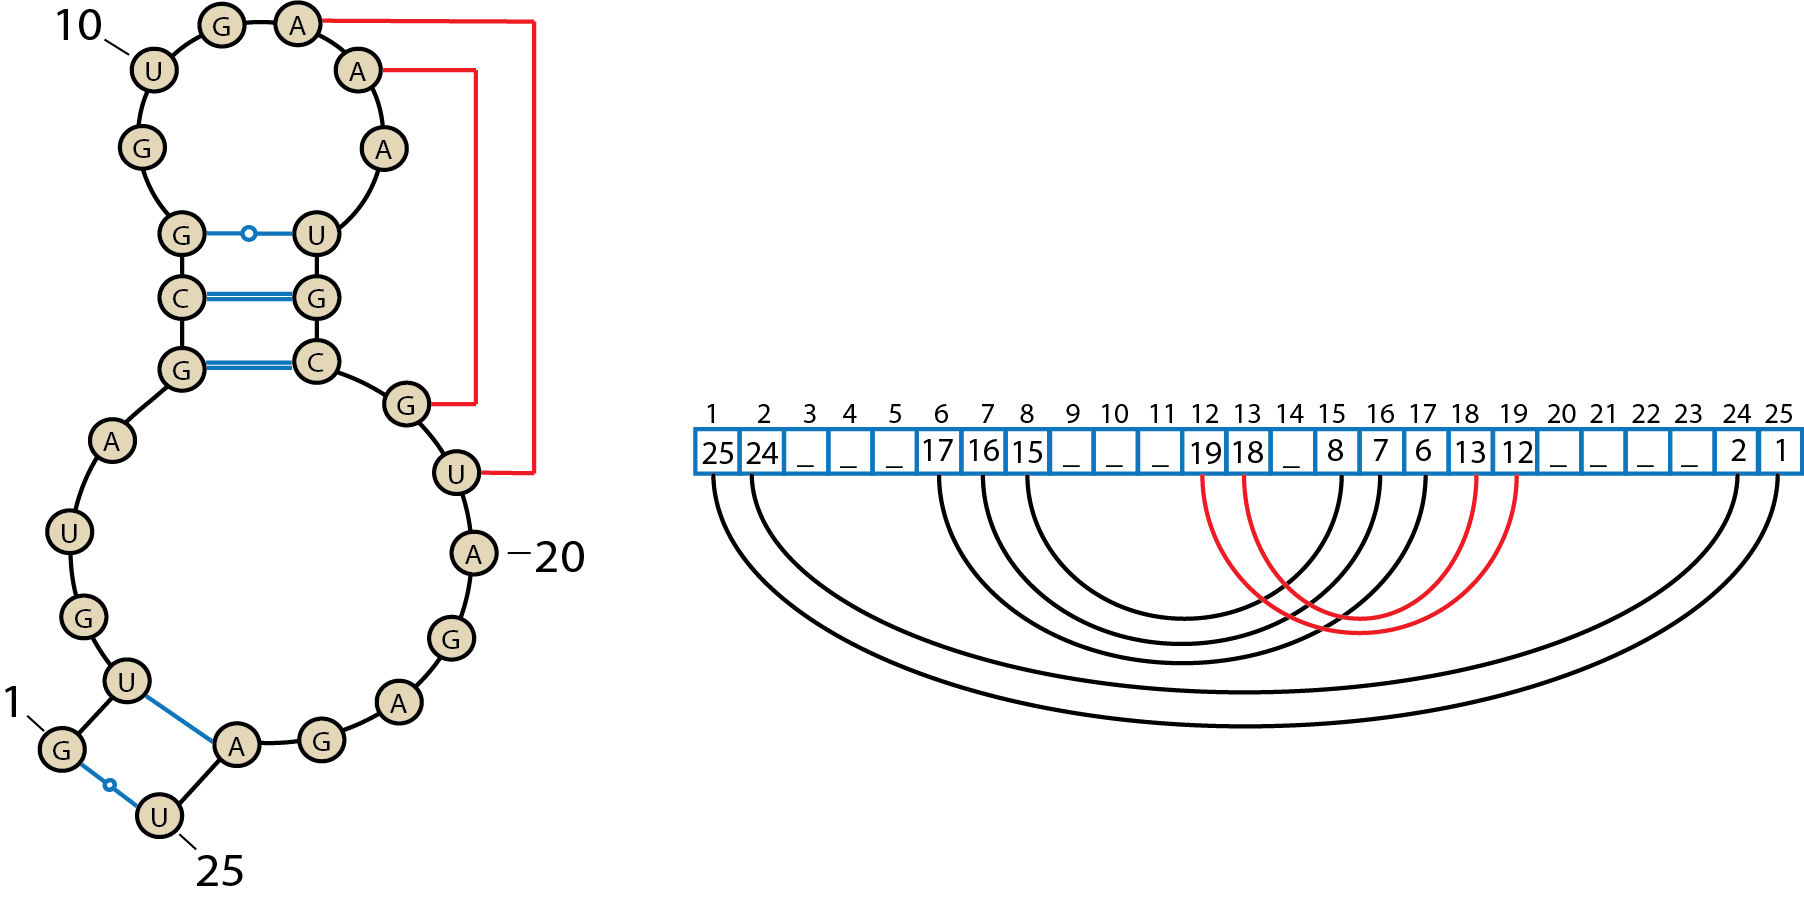
\includegraphics[width = \textwidth]{./pictures/PseudoKnotArchs.png}
\caption{Secondary structure of an exemplary RNA molecule and its list-representation. Red lines correspond to the WC interactions creating a pseudo-knot.}
\label{SecondaryStructureList}
\end{figure}

\paragraph{Pseudo knots}
The list-representation contains also the information about the non-secondary motifs. The pseudo-knot is formed by the WC interactions but creates three-dimensional folds as shown in Figure \ref{PseudoKnot}. Our program detects the pseudo-knot fold when the arcs intersect. A pseudo-knot is a symmetric structure so both the pairs 6--17, 7--16, 8--15 and 12--19, 13--18 in Figure \ref{SecondaryStructureList} form a pseudo-knot. The natural way of solving this conflict is to choose the shorter list, in this case the pairs 12--19 and 13--18.
  
\begin{figure}[h!]
\begin{center}
\subfigure[Tertiary structure]{
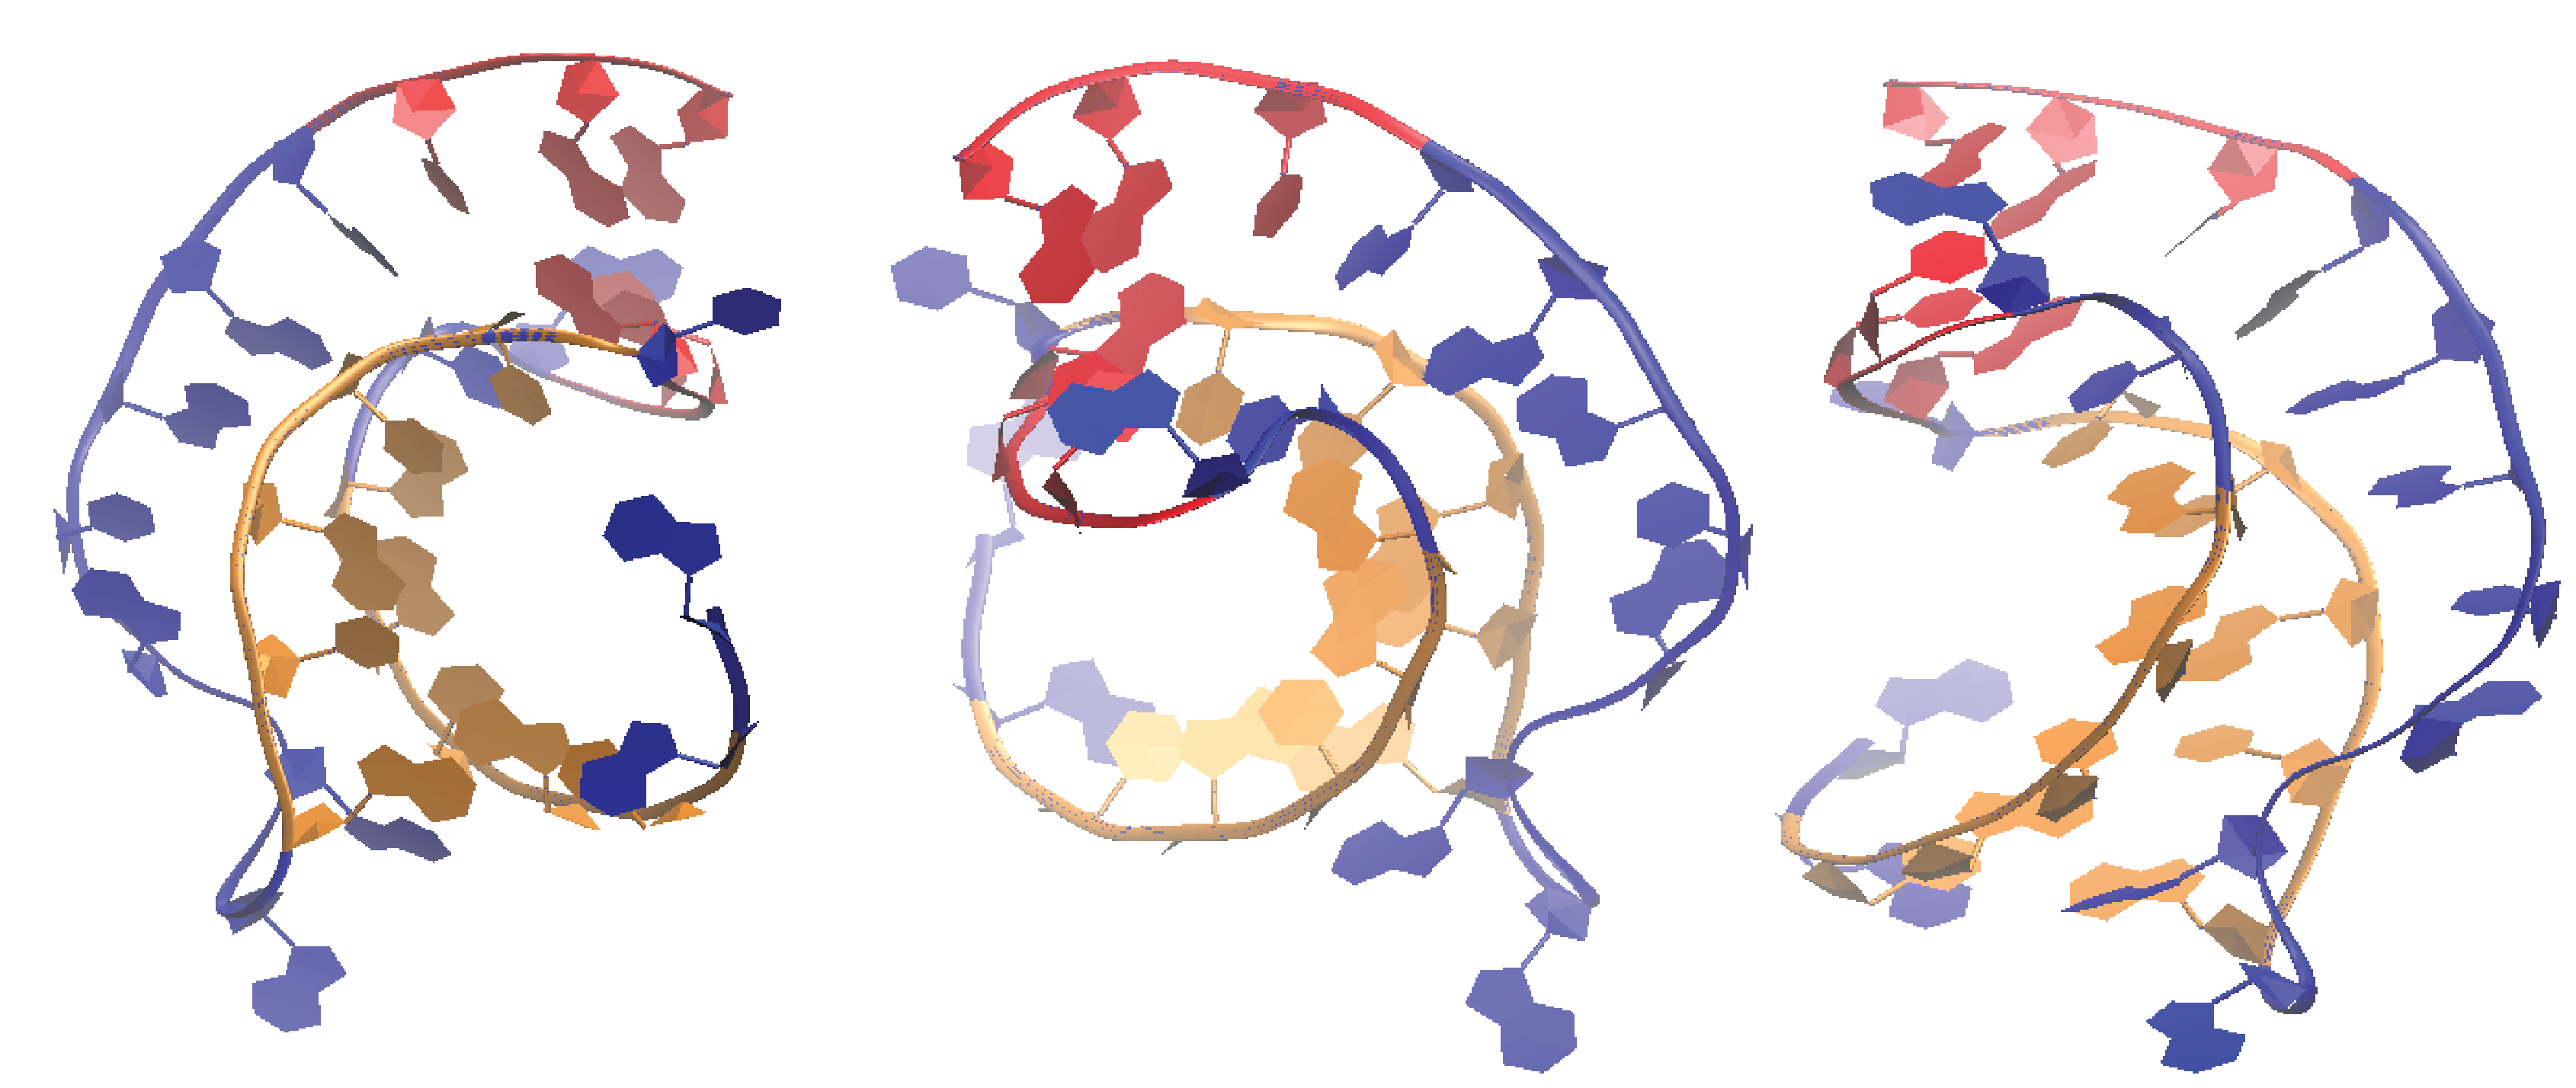
\includegraphics[width=12.5cm]{./pictures/pseudo_knot_combo.png}}
\subfigure[Secondary structure]{
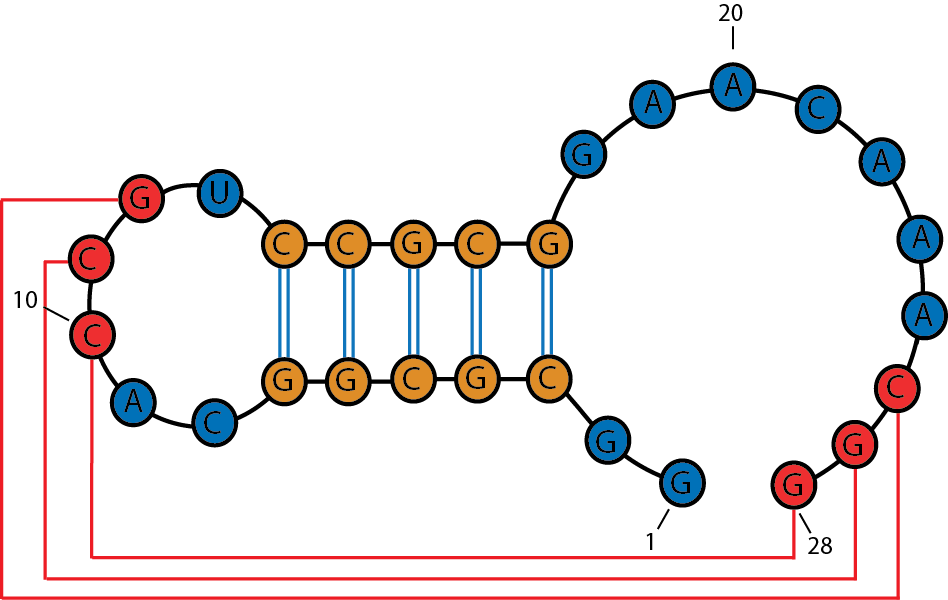
\includegraphics[width=6cm]{./pictures/pseudo_secondary_structure.png}}
\end{center}
\caption{An example of the RNA structure with a pseudo-knot seen from three different angles. Nucleotides colored in red create a pseudo-knot, orange form a helix and blue refer to loops (PDB id: 437d).}
\label{PseudoKnot}
\end{figure}
\newpage

After detecting all pairs and creating a list, {\tt MINT} finds all pseudo-knots and erases them from the list by putting the \texttt{None} value. Next, it looks for all other kinds of motifs, that are defined as a set of unpaired nucleotides surrounding the paired nucleotides as shown in Figure \ref{MotifDesc}.

\begin{figure}[h!]
\centering
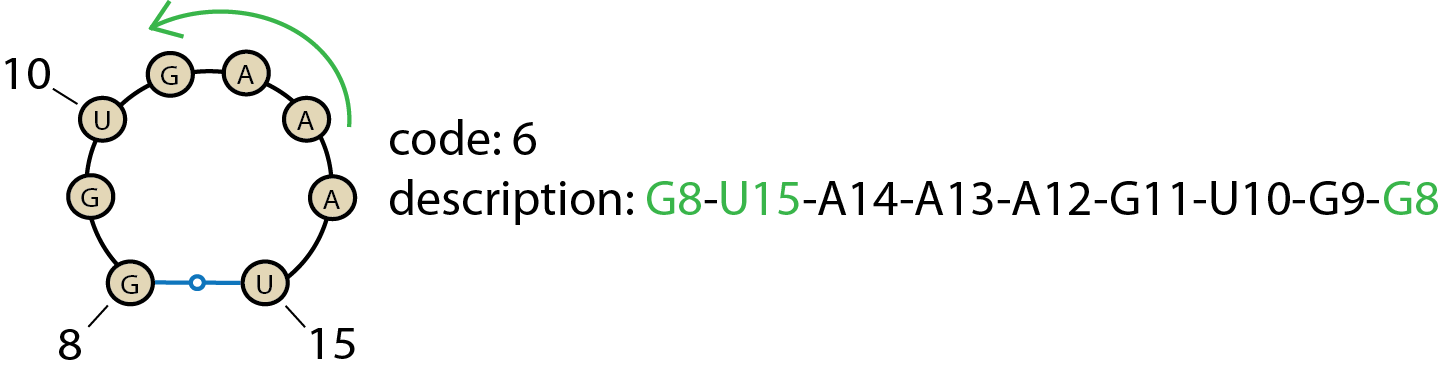
\includegraphics[width = \textwidth]{./pictures/motifs_description.png}
\caption{The program denotes the first pair (shown in green) and then makes a list of unpaired nucleotides. Nucleotides are listed in the counter-clockwise direction.}
\label{MotifDesc}
\end{figure}

\begin{table}
\caption{RNA secondary structure motifs}
\label{RNAsecondaryStructures}
\begin{tabular}
{ >{\centering} p{5.5cm} >{\centering} p{5.5cm} >{\centering} p{5.5cm}}
&& \tabularnewline
 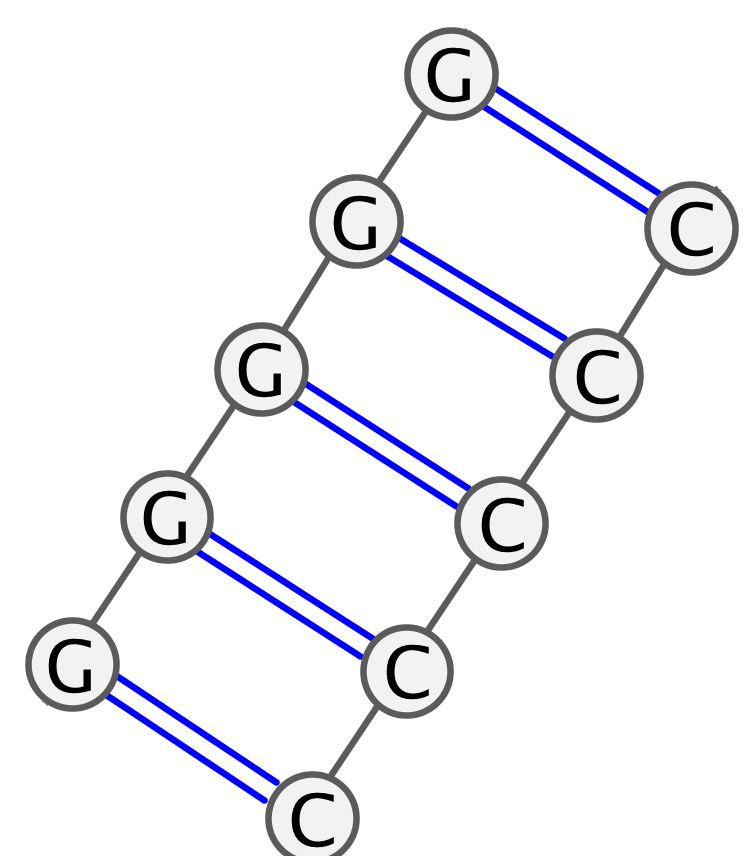
\includegraphics[width=4.5cm]{./pictures/helix_varna.PNG}  \linebreak Helix 
 & 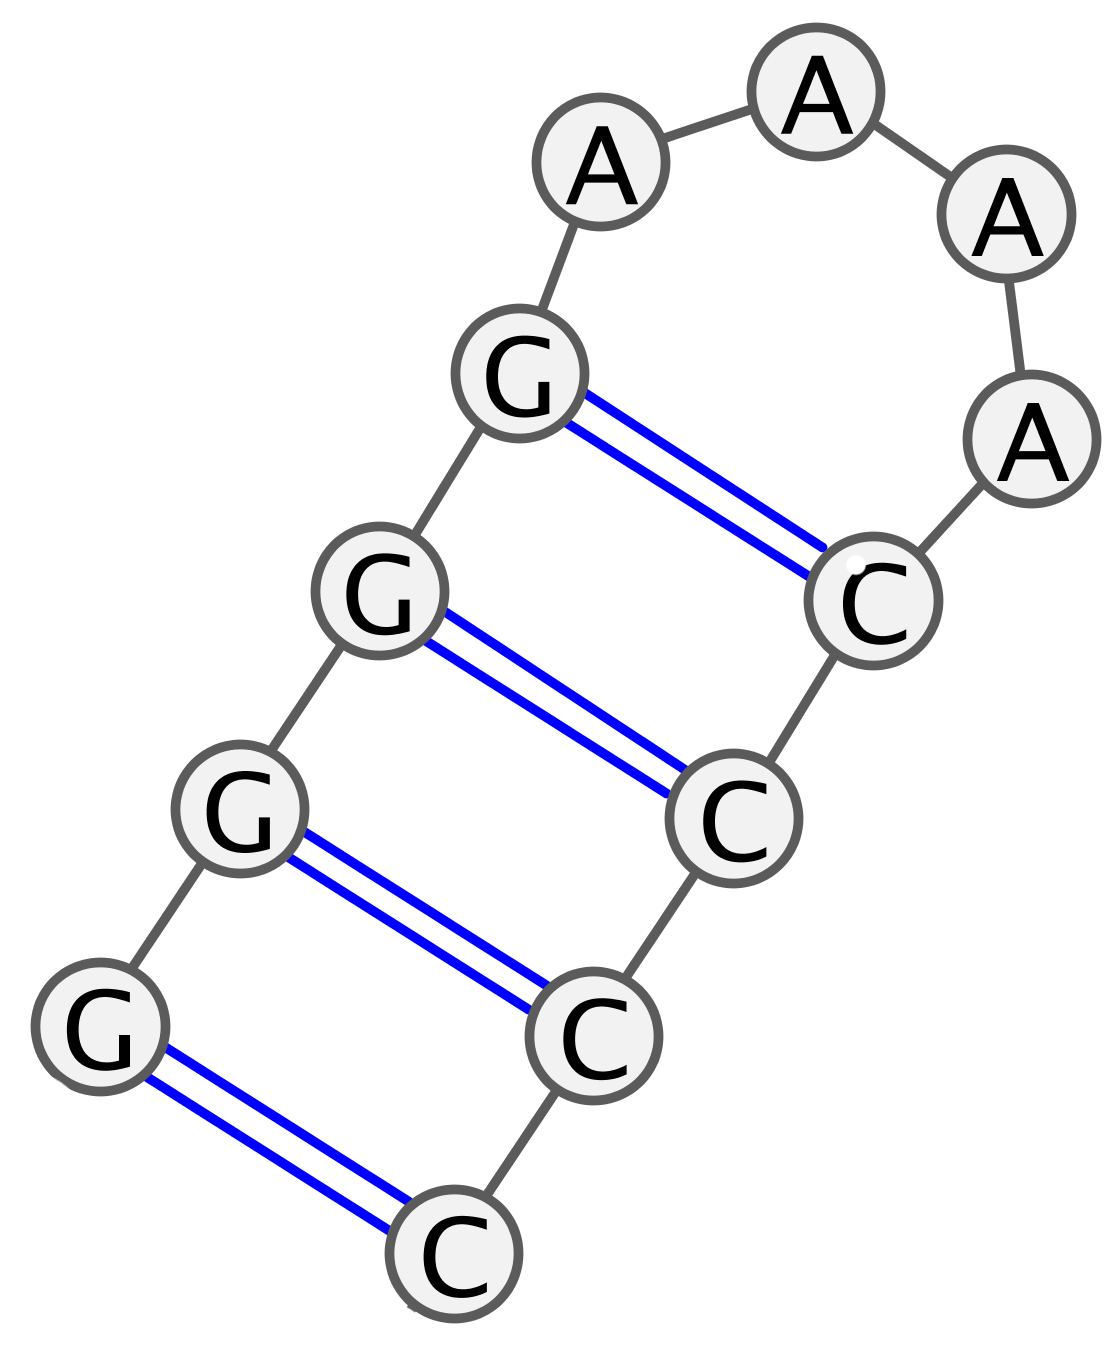
\includegraphics[width=4.5cm]{./pictures/hairpin_varna.PNG}  Hairpin loop \linebreak (code: 4) &  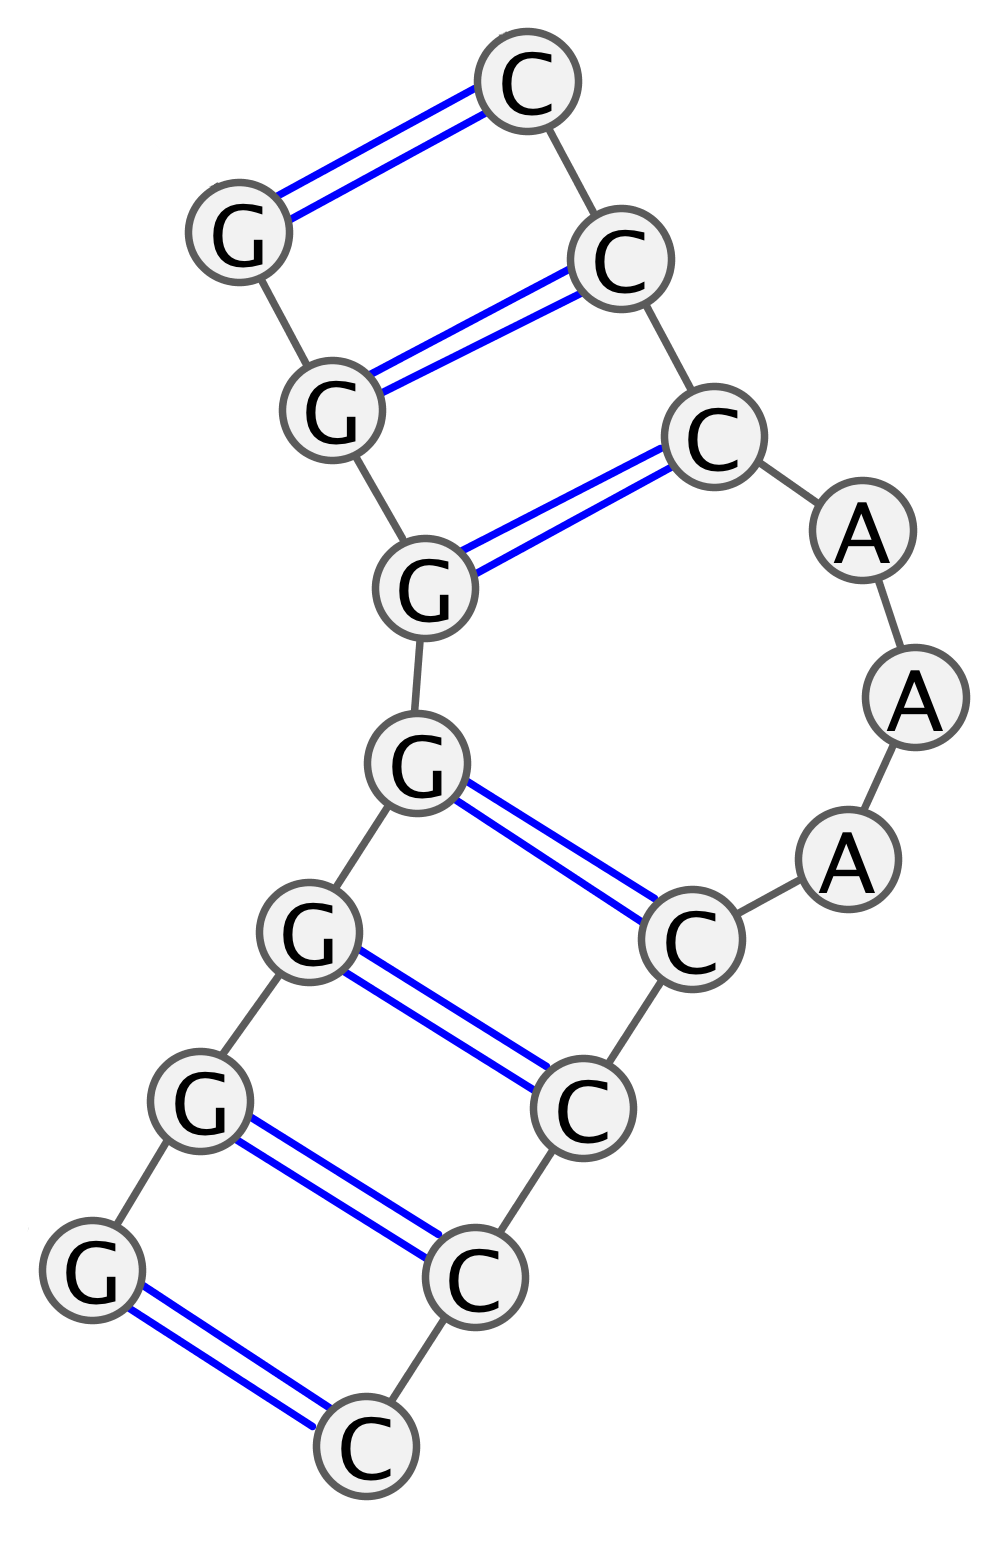
\includegraphics[width=4.5cm]{./pictures/bulge_varna.PNG} Bulge loop\linebreak  (code: 0--3) \tabularnewline
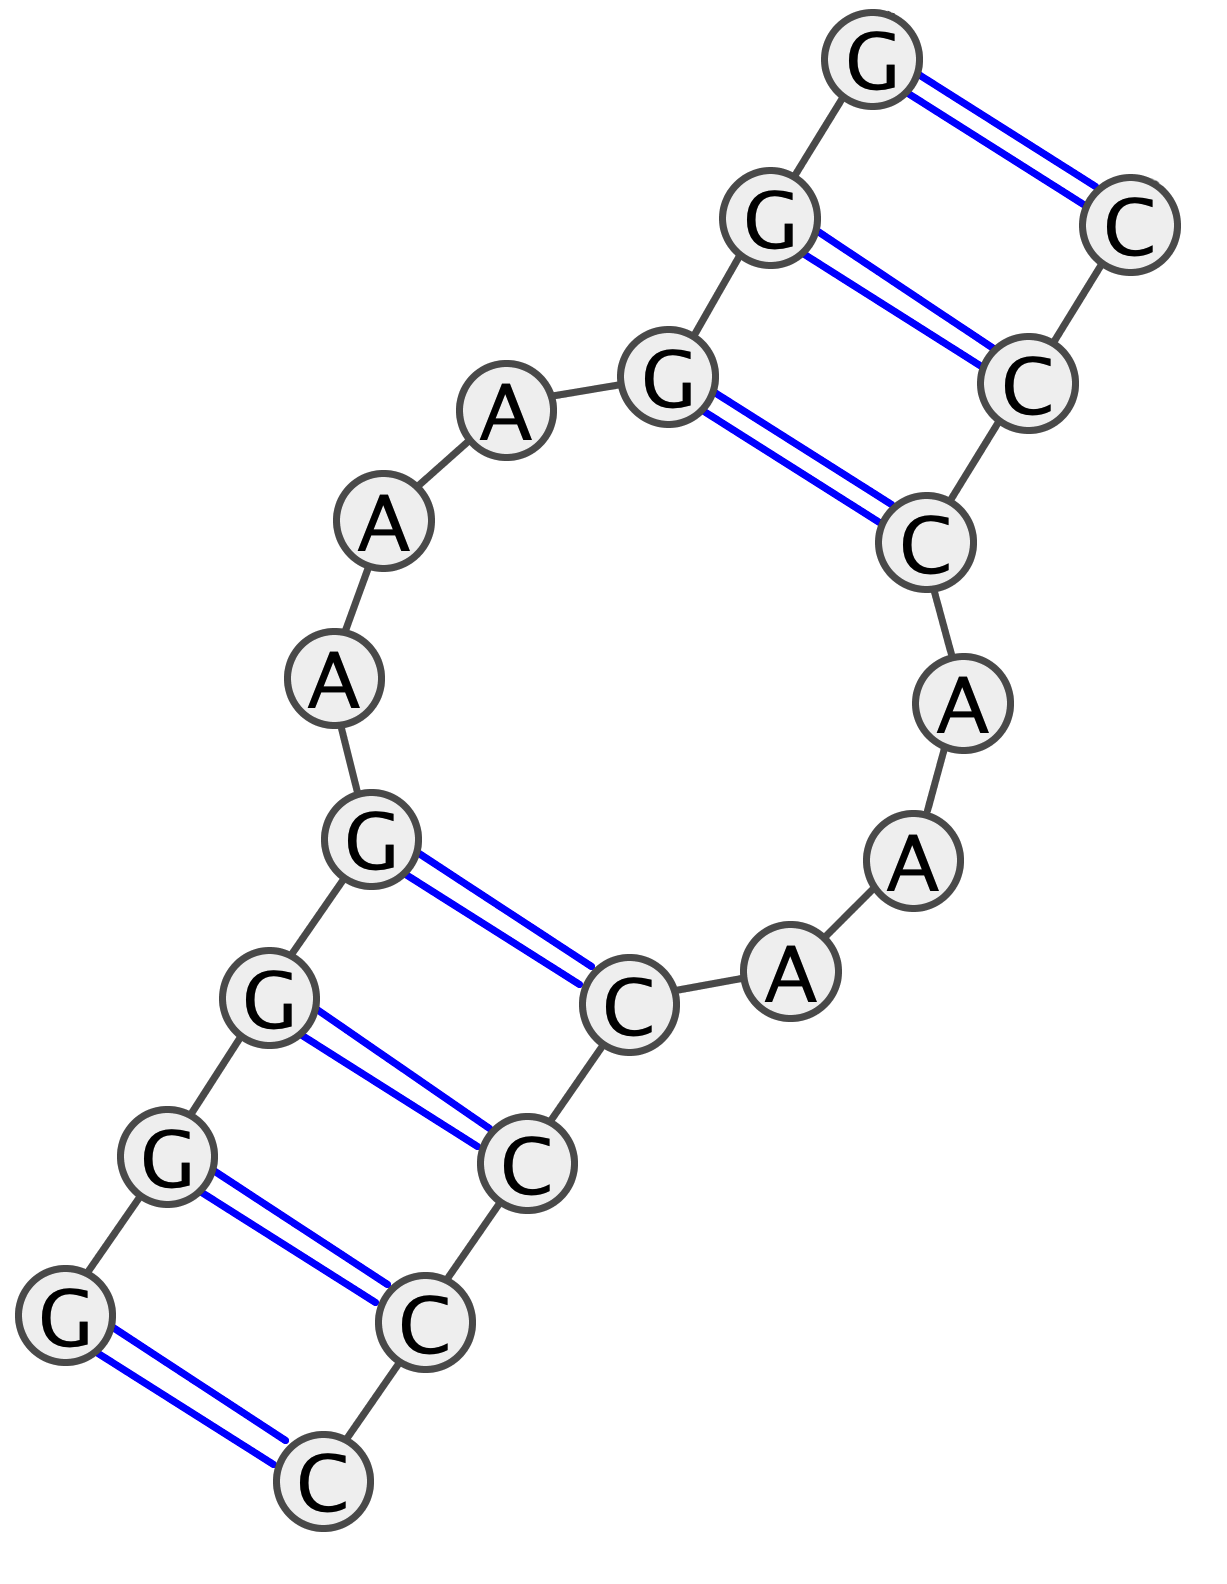
\includegraphics[width=5cm]{./pictures/interior_varna.PNG} Interior loop \linebreak  (code: 3--3) & 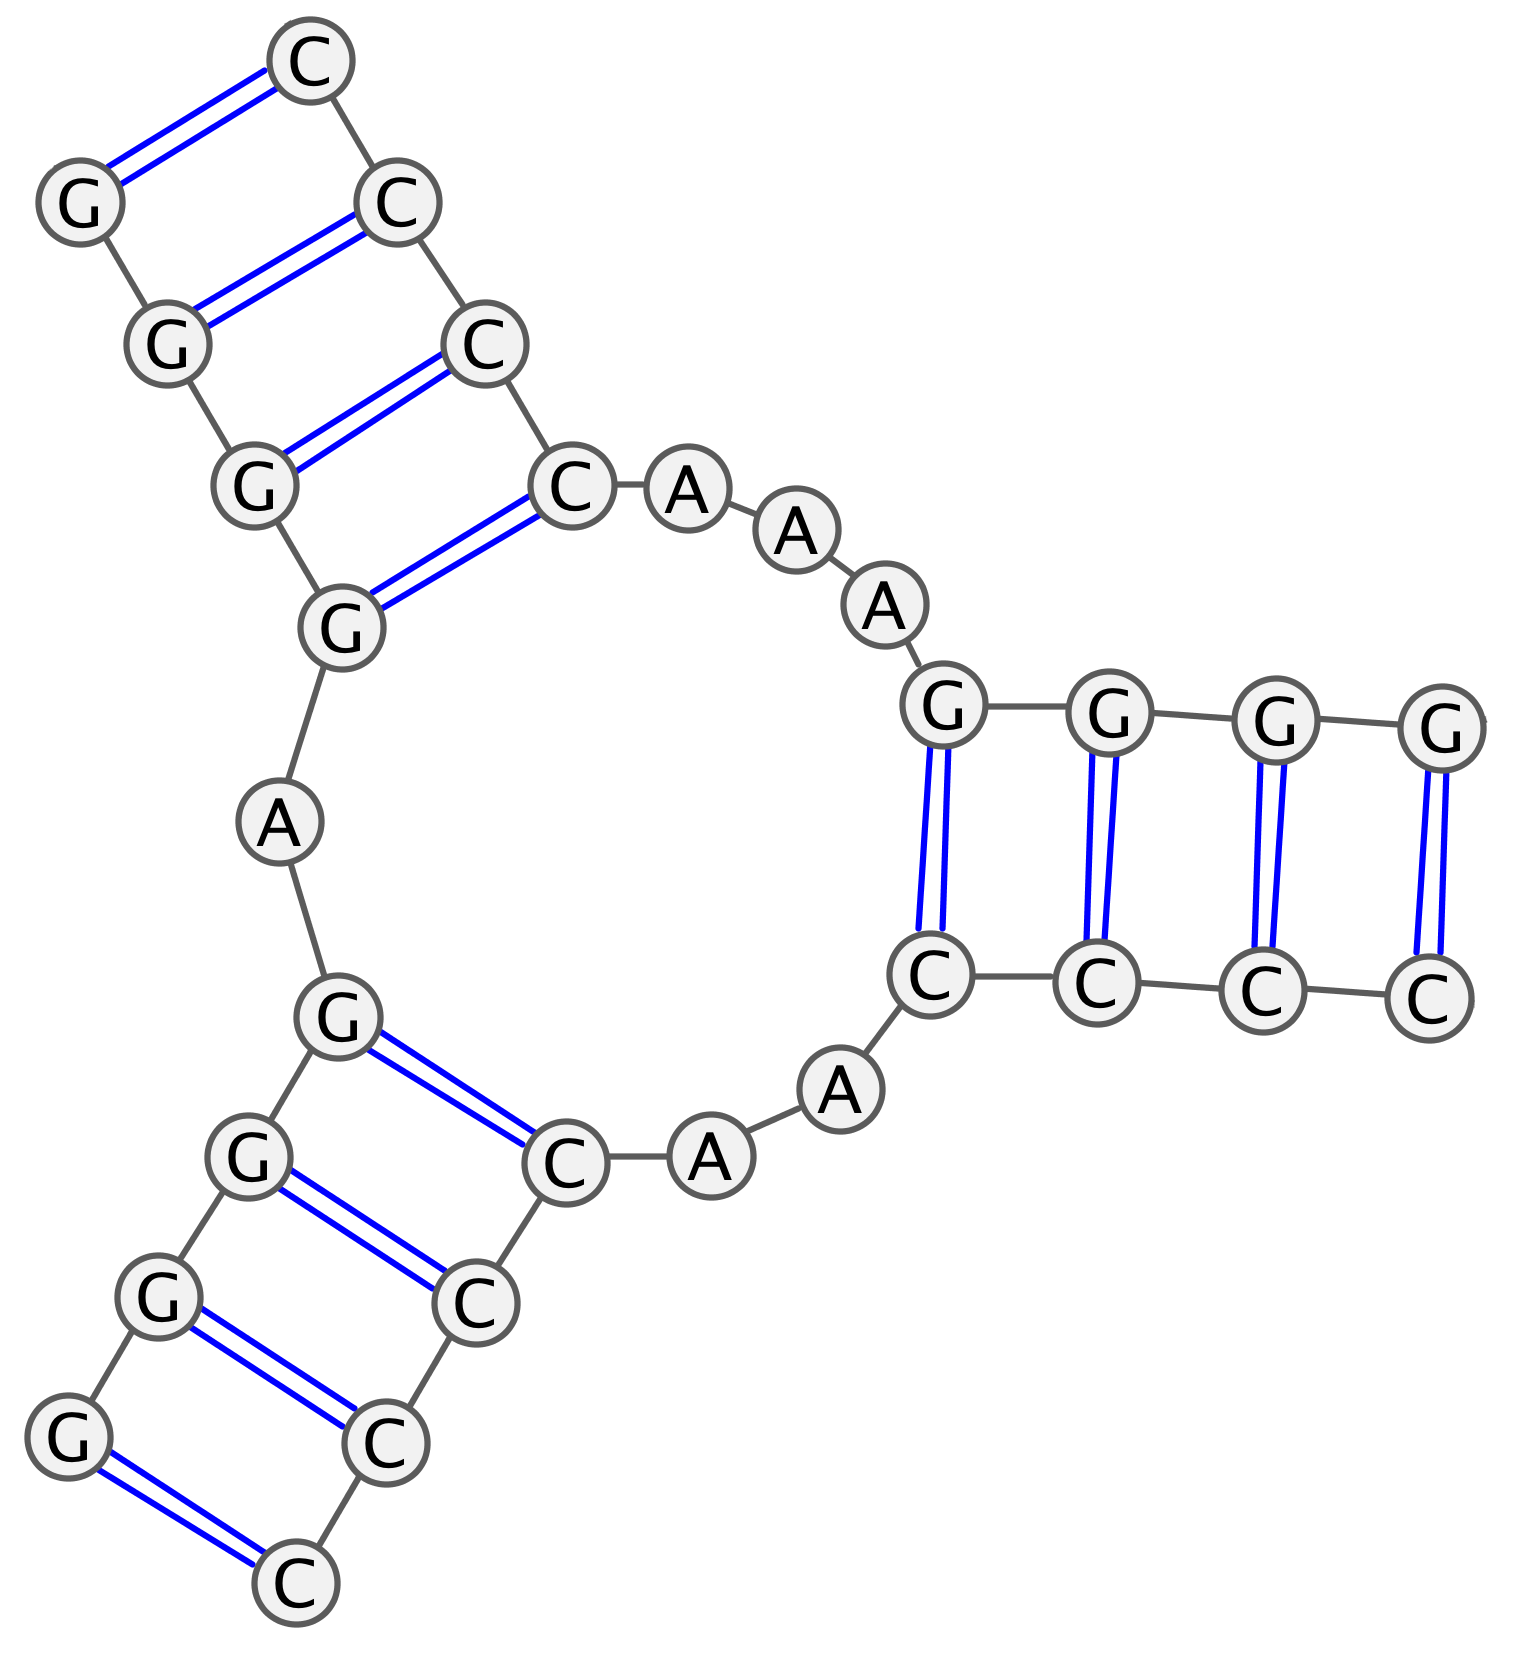
\includegraphics[width=5.5cm]{./pictures/multibranched_varna.PNG} Multi-branched loop\linebreak (code: 2--3--1) & 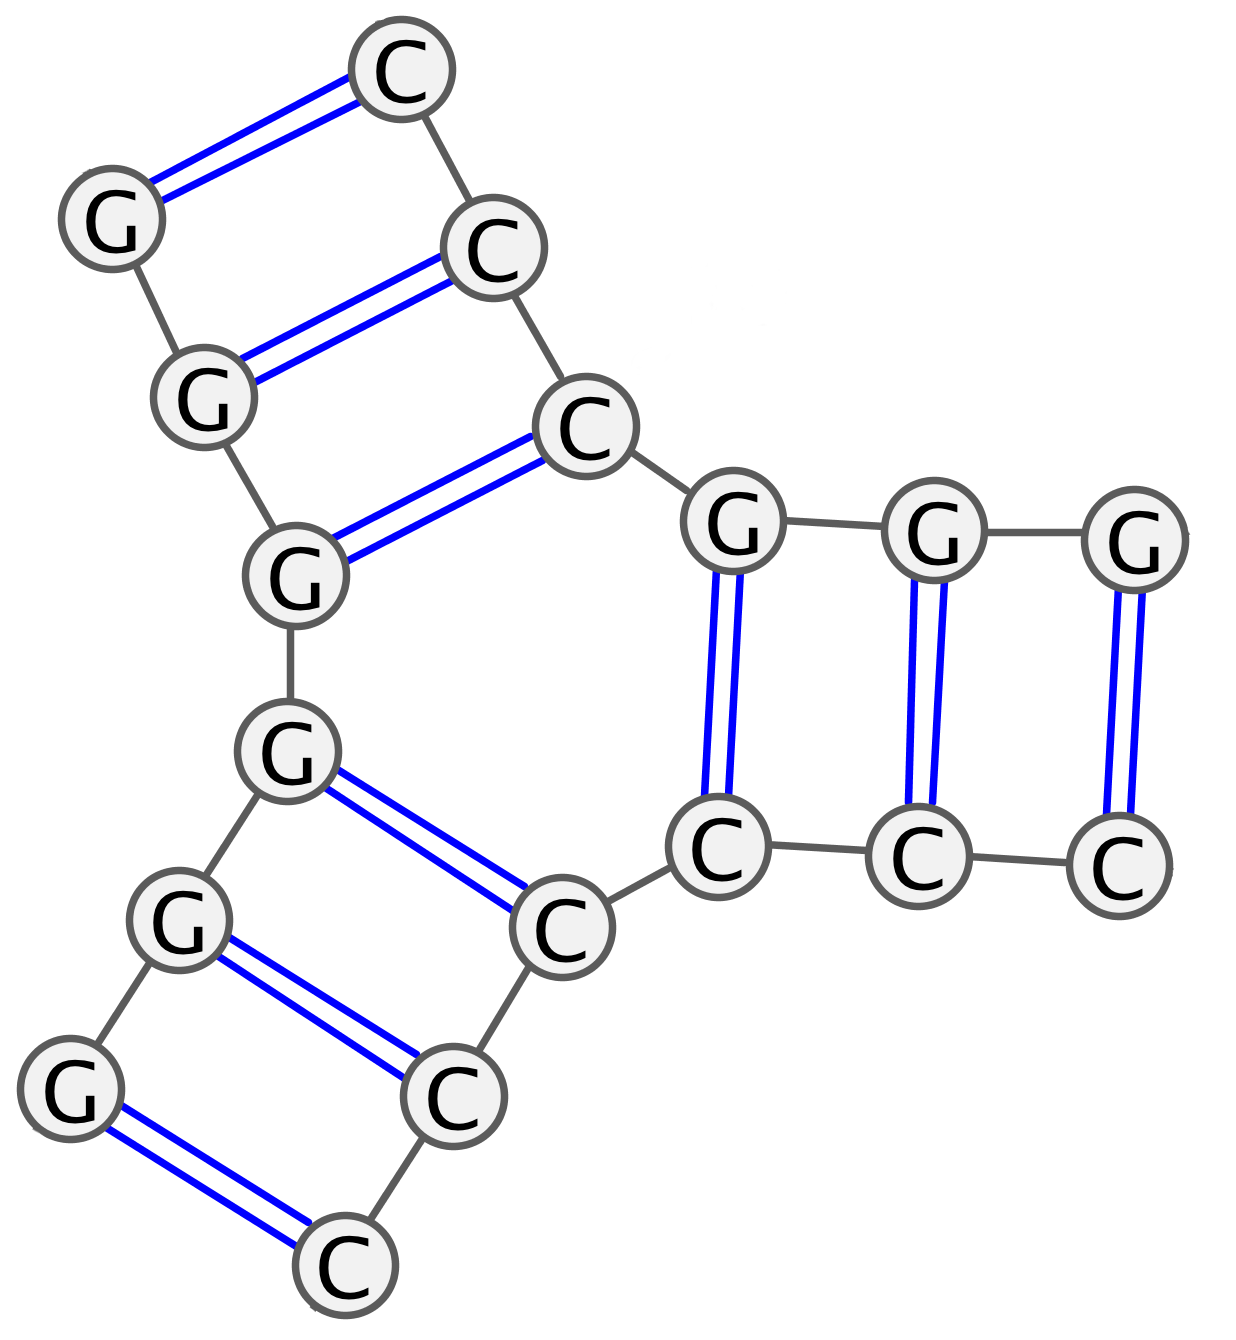
\includegraphics[width=5cm]{./pictures/junction_varna.PNG} 3-way junction\linebreak (code: 0--0--0)  \tabularnewline
&& \tabularnewline
\end{tabular}
\end{table}

\newpage

\paragraph{The RNA motif} \label{RNA_motifs} nomenclature (i.e., a loop, bulge or junction) can be inaccurate and misleading. The program uses the numerical description of motifs that should be easily understandable. The numbers correspond to the numbers of unpaired nucleotides between the paired nucleotides. Therefore, a four nucleotide loop at the end of a hairpin is represented by a single number 4. A symmetric bulge loop, with both bulges of the length of three is represented by two numbers: 3--3 and a three-way junction, without unpaired nucleotides is represented by three zeros: 0--0--0.  Examples of RNA secondary structure motifs with their labels are presented in Table \ref{RNAsecondaryStructures}. 

\subsection{Motif-search algorithm}
The motif-search algorithm uses a list-representation of the RNA-secondary structure that contains the list of all WC pairs. As shown in Figure \ref{MotifsAlgorithm} the algorithm detecting helices and other secondary structure motifs walks through the list and stores the information about the visited nucleotides. 

As long as there are paired nucleotides, the algorithm stores the information about the helix (steps 1 and 15 in Figure \ref{MotifsAlgorithm}). When it encounters the end of the helix (steps 2 and 16) -- i.e., an unpaired nucleotide ahead of a pair, it starts to travel (search) around the motif. It stores the first pair (as the beginning pair) and goes to the index stored in the list. Then for as long as it encounters an unpaired nucleotide it moves back -- with decreasing indexes (steps 3 to 13 and steps 16 to 22). When another pair is encountered, the algorithm goes into the indicated position and again moves back (steps 10 and 16). This motif-search ends when the algorithm finds itself one step ahead of the starting index (steps 13, 22). The number of "jumps" represents the number of unpaired nucleotides in between. After one motif is found and classified, the algorithm jumps one step further to the last seen pair (steps 14 and 23). The algorithm stops searching for the motifs and helices when the index is larger than the value stored in the list (step 23). 

\begin{figure}[h!]
\centering
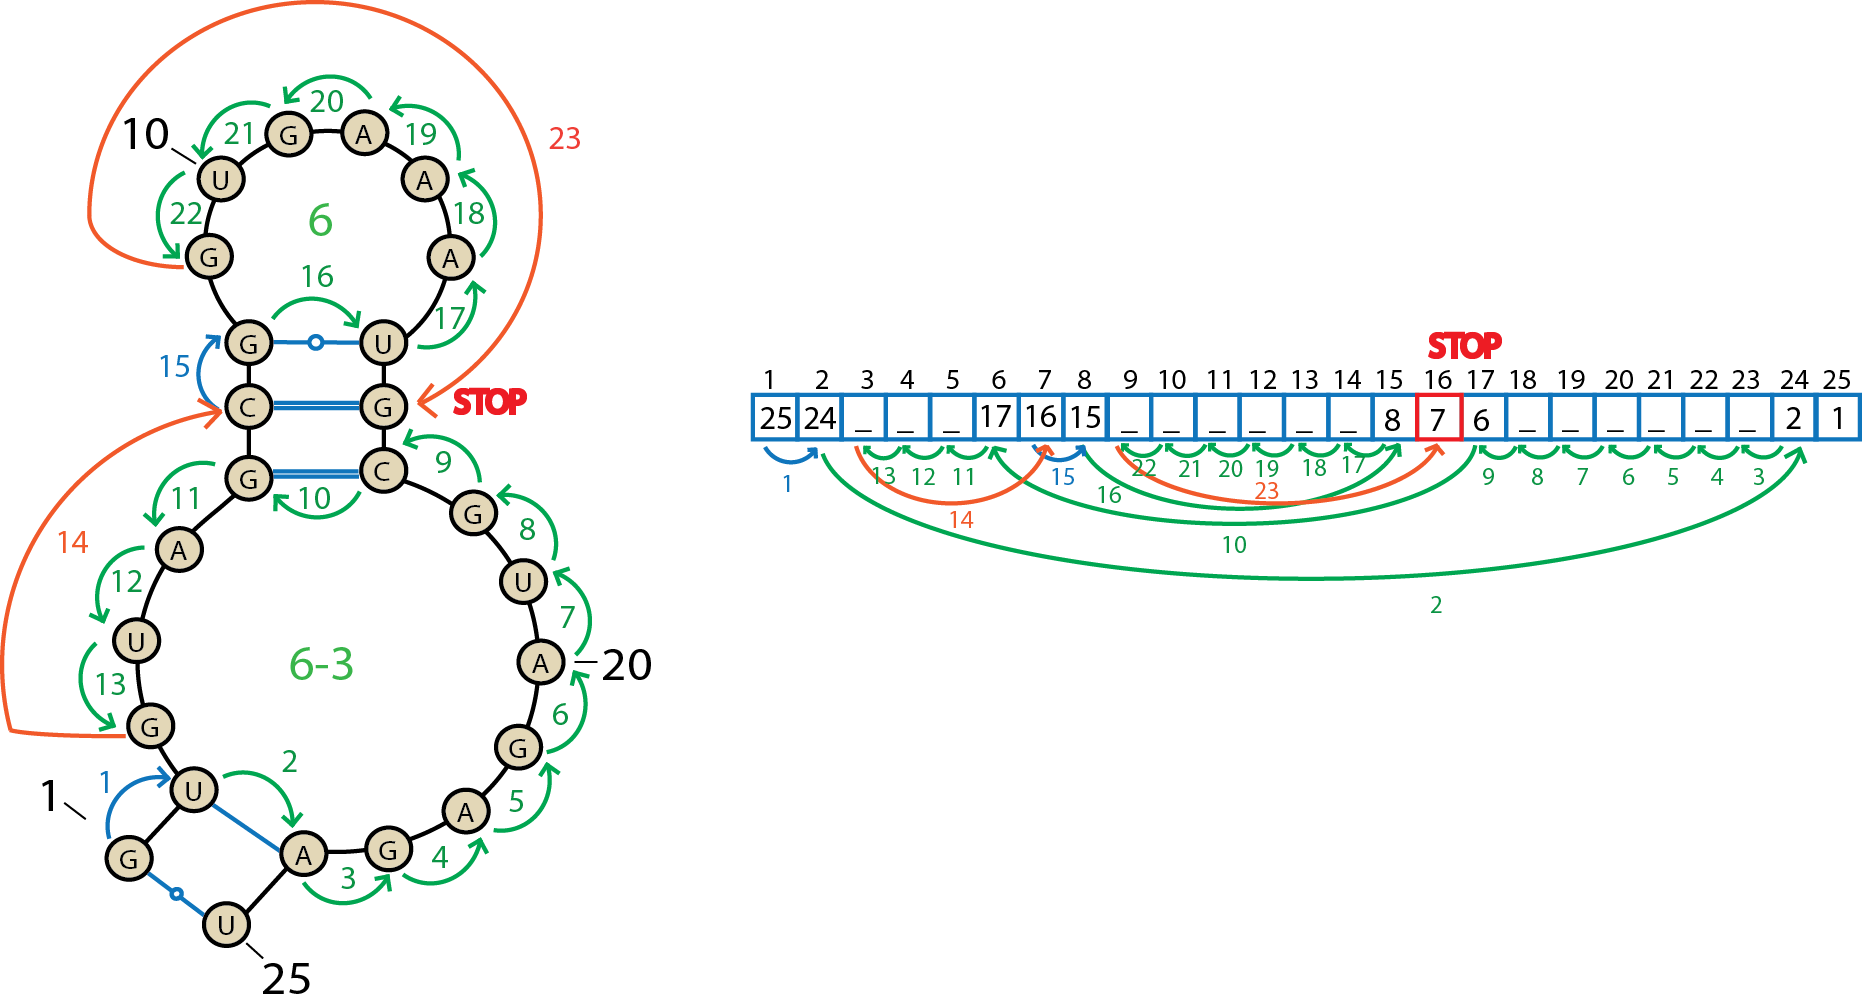
\includegraphics[width =\textwidth]{./pictures/algorithm.png}
\caption{A scheme presenting the steps of the algorithm that finds and classifies the motifs in the RNA structures. The numbers correspond to the step number. Green arrows correspond to the structural motif and blue to  helices. The orange lines denote the jumps after finishing the motif. The STOP sign indicates the position where the algorithm stops.}
\label{MotifsAlgorithm}
\end{figure}

As a result of a single frame analysis, the algorithm returns a list of all pairs, motifs and numerical characterization of all nucleotides. Every nucleotide is characterized with the number of hydrogen bonds it created and the description of its partners:

\begin{verbatim}
G538 , 538 , 3-C513A539:1 , 2-C513:2 , 3-C513:7
\end{verbatim}

where first comes the type of the nucleotide with its PDB id, second only the PDB id, followed by the lists of pairs this nucleotide created during the trajectory or in the uploaded conformation set. The number of hydrogen bonds is preceding the hyphen. Next, there can be more than one nucleotide listed -- what indicates a triplex. The number after a semicolon is the number of frames in which this pair or triplex were detected.

\newpage
\section{Analysis of trajectories or many RNA/DNA conformations}
If multiple RNA/DNA conformations (e.g. from molecular dynamics trajectory) have to be analyzed and classified, every frame/conformation is characterized as previously described. The main output of the program is a set of \texttt{.csv} files listing all the pairs and motifs: helices, triplexes, pseudo-knots etc., their occurrence and frame numbers in which the considered structure was present, its topology and participating nucleotides. Description of the output files can be found in Section~\ref{OutputFiles}.

\subsection{Clustering}
To recognize and characterize the changes in the secondary structure of the RNA/DNA molecule that may occur in the trajectory, we have to cluster the detected secondary structure motifs. Clustering is parameterized with two user-defined parameters: \\
\begin{itemize}
\item \texttt{time\_cutoff} that defines the minimal percentage of frames in which the motif has to be present in order to be classified.
\item \texttt{margin} that defines the minimal percentage of similarities between the two motifs to belong to the common cluster. 
\end{itemize}

The first step is to filter the motifs i.e., remove the rare motifs  and leave only the significant ones. Filtering of motifs is done according to the number of frames the motif appeared in. Below we show an exemplary list of motifs after removing rare motifs:

\begin{figure}[h!]
\centering
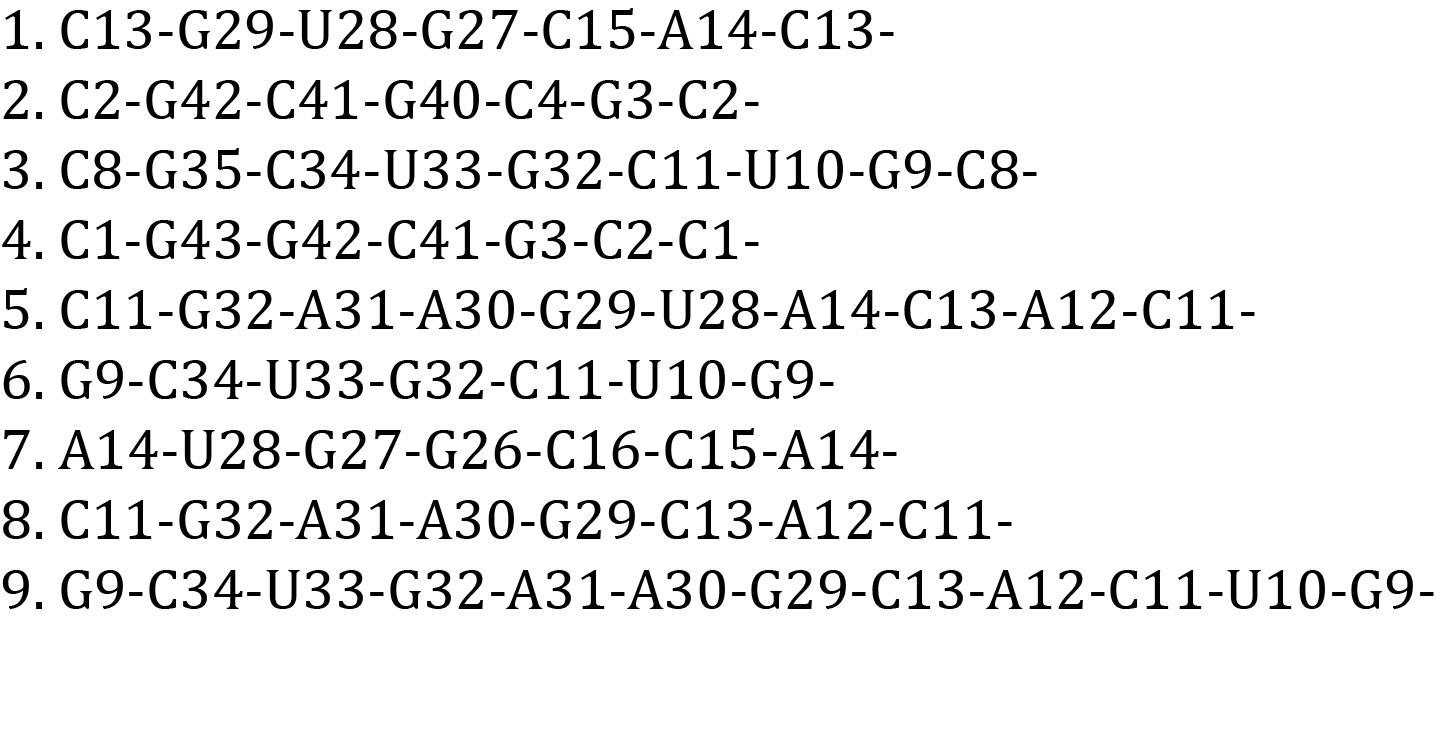
\includegraphics[scale=1]{./pictures/cluster_motif_step1.png}
\caption{First step of clustering.}
\label{MotifsClusteringStep1}
\end{figure}

Second, the motifs' distance matrix is computed. The distance between the motifs is the number of their common nucleotides. The order of the nucleotides is not taken into account:
\begin{figure}[h!]
\centering
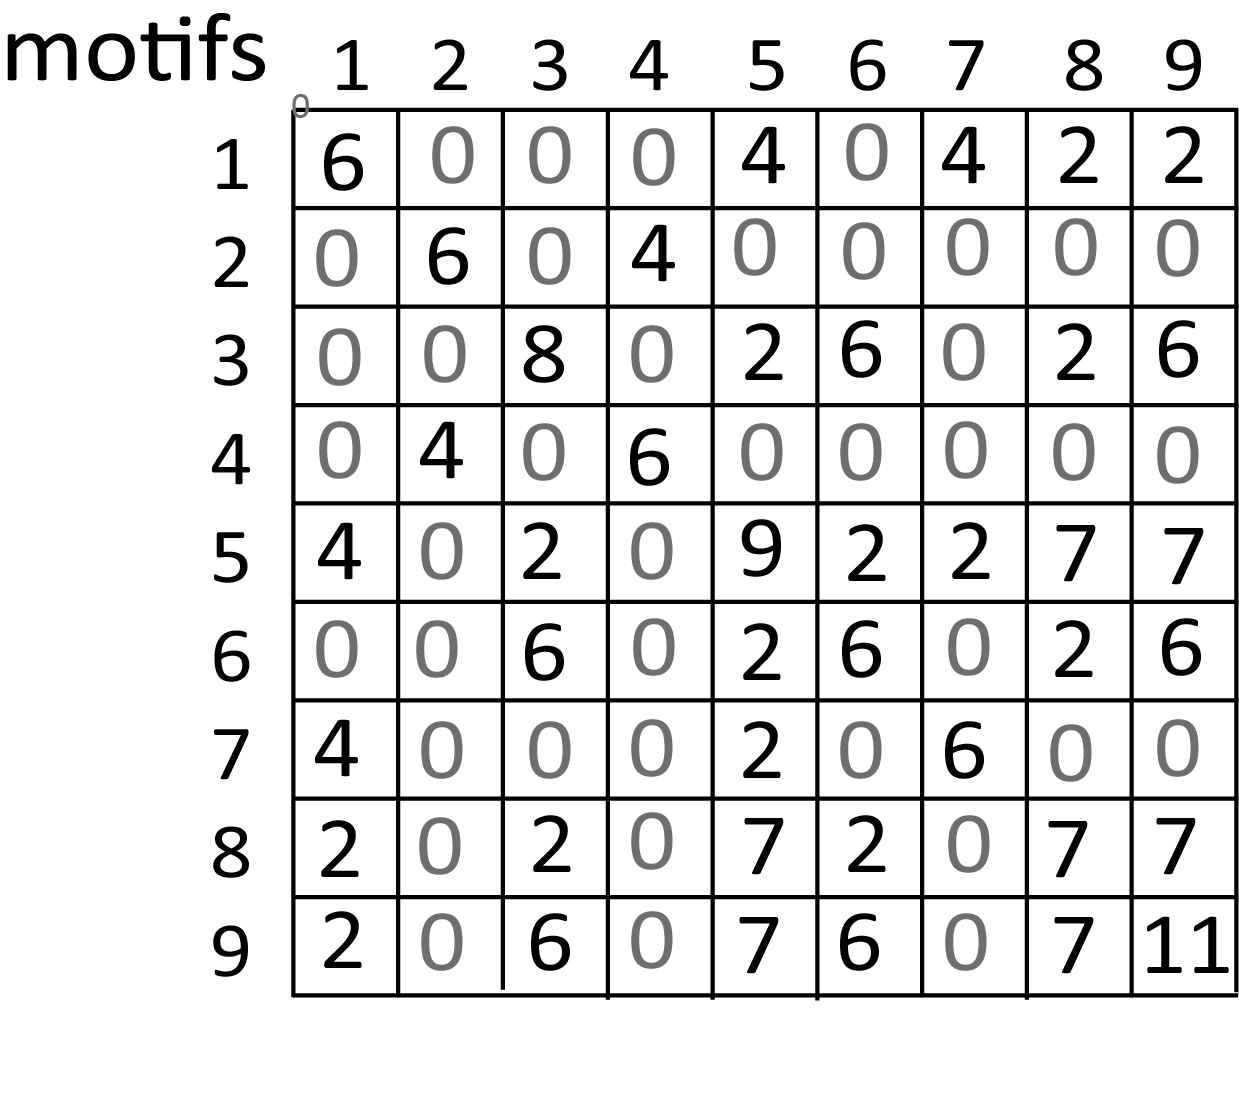
\includegraphics[scale=0.6]{./pictures/cluster_motif_step2.png}
\caption{Exemplary motif distance matrix}
\label{MotifsClusteringStep2}
\end{figure}

\newpage
Third, the partners for all motifs are denoted. The partner has to satisfy the distance requirement expressed by the equation shown below:
\begin{figure}[h!]
\centering
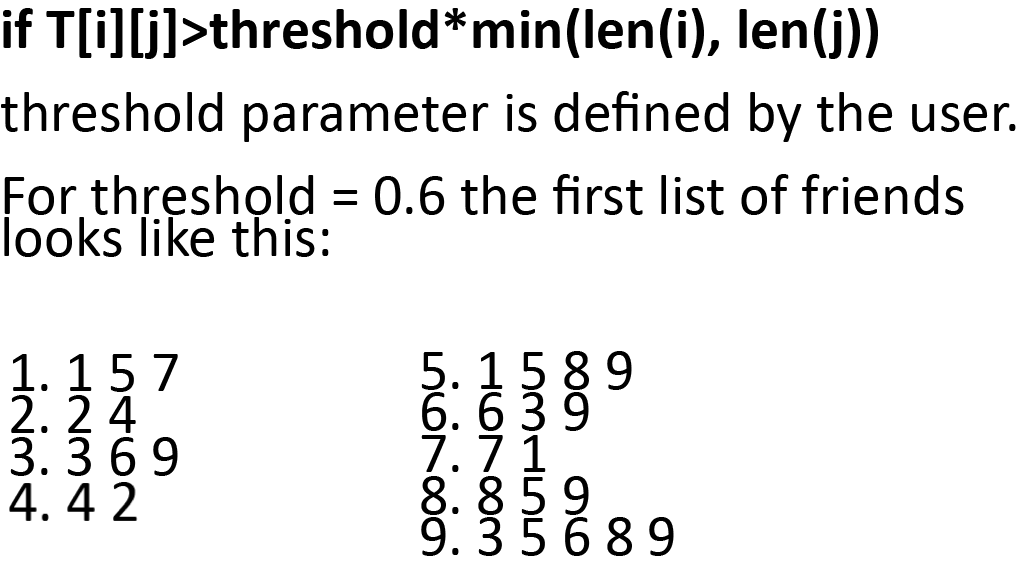
\includegraphics[scale=1]{./pictures/cluster_motif_step3.png}
\label{MotifsClusteringStep3}
\caption{Equation with the distance requirement that motifs have to satisfy to be partners}
\end{figure}

Next, the motif with the longest list of partners is incorporated as the first one to the first cluster (numbered zero). The motifs already assigned to the first cluster have to be crossed out from the rest. Then the second longest motif is chosen, the picked motif is crossed out, and so on.  

\begin{figure}[h!]
\centering
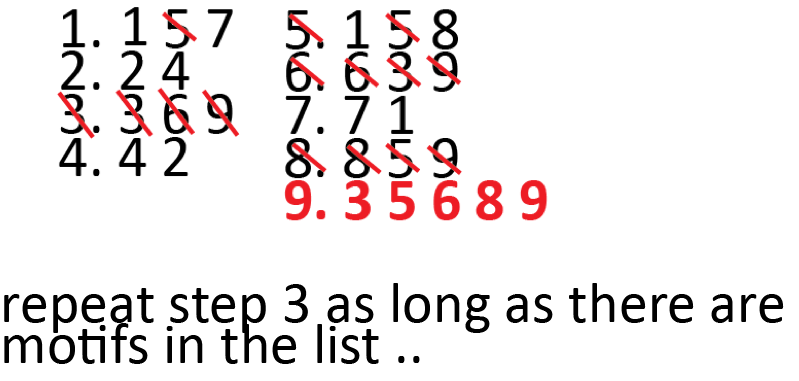
\includegraphics[scale=1]{./pictures/cluster_motif_step4.png}
\label{MotifsClusteringStep4}
\caption{Removal of partners from the list of motifs}
\end{figure}

\begin{figure}[h!]
\centering
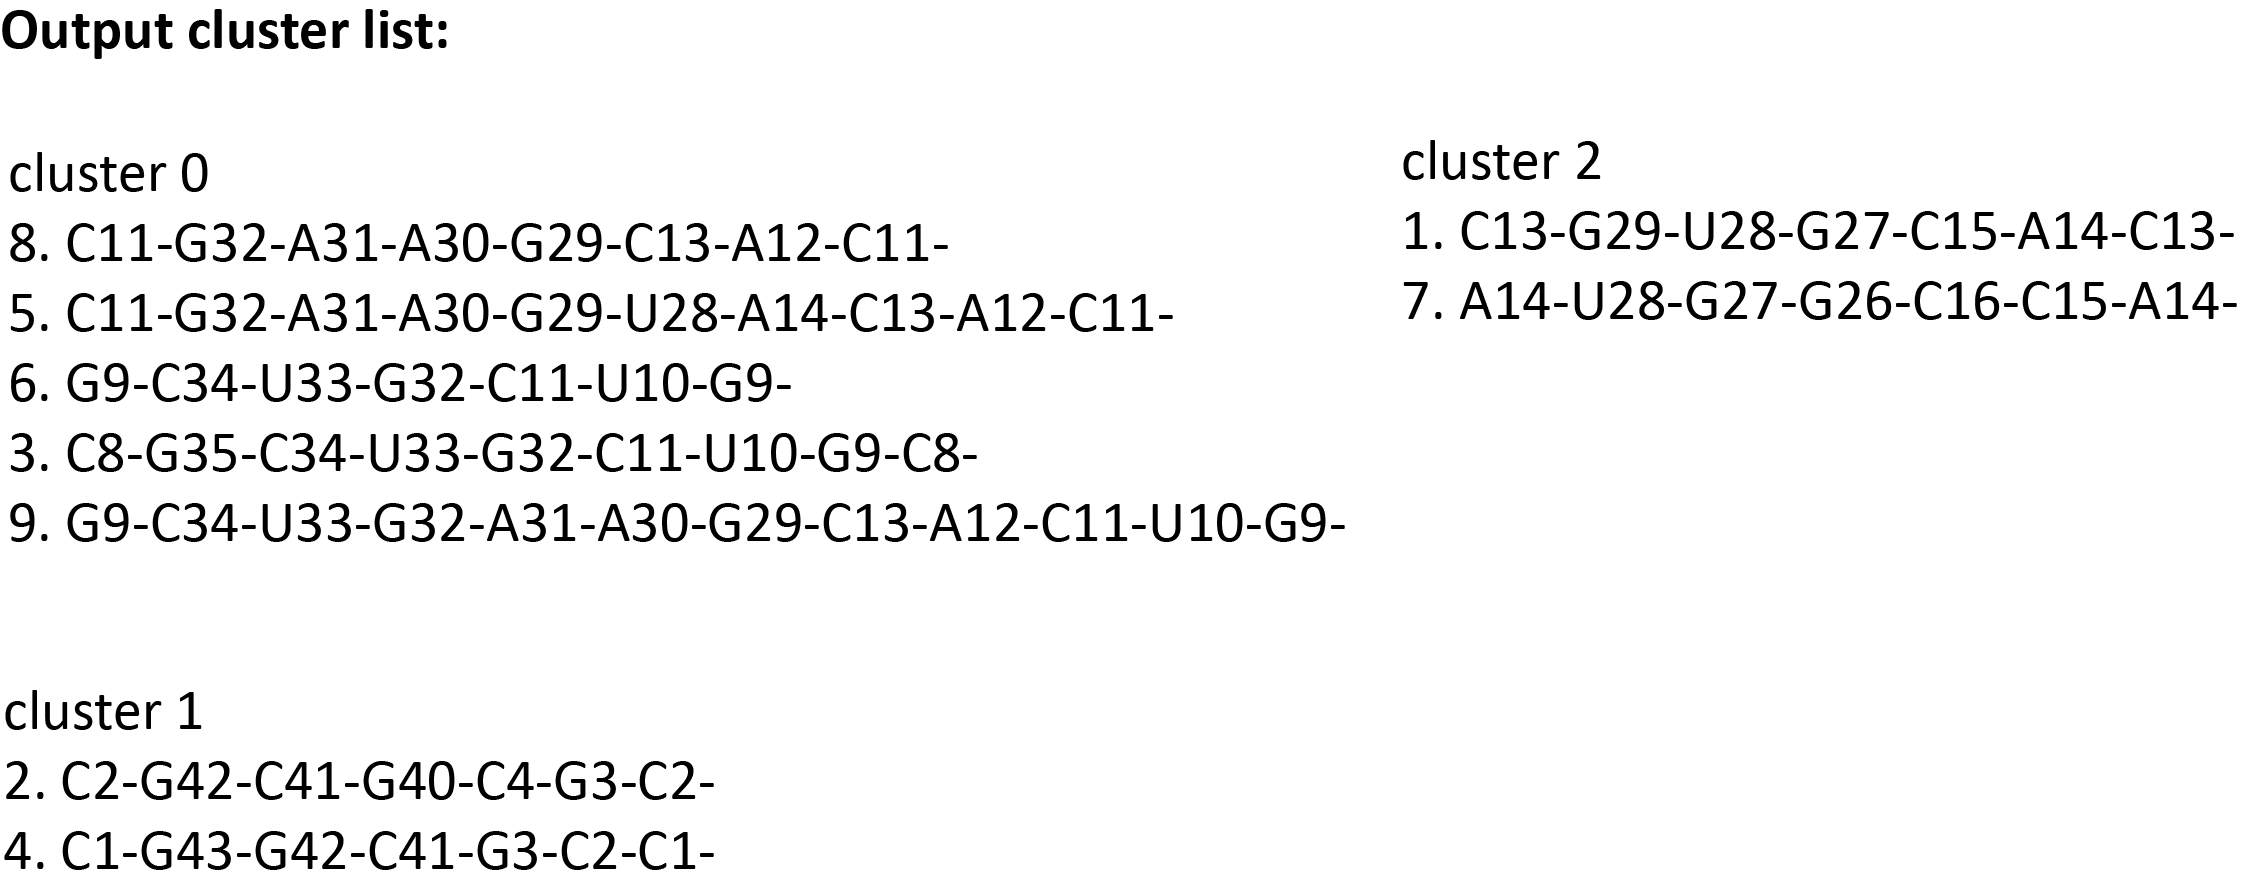
\includegraphics[scale=1]{./pictures/cluster_motif_step5.png}
\label{MotifsClusteringStep5}
\caption{Result of the clusterization process.}
\end{figure}

Additionally, the average clusters are returned. The list consists of the longest motif for every cluster and the two vectors of float values describing every nucleotide participating in the representative motif. The float vectors represent the average number of hydrogen bonds created by a nucleotide in both WC-WC pairs and other interactions. We hope to show the average secondary structure of the molecule within the tertiary structure description. While analyzing the whole output generated by the script, one can understand the complex description of the RNA structure in the dynamics.

% Visualization - odnosnik do VMD gdzies sie powinien pojawic.

\section{Visualization}\label{Visualization}
MINT enables many different ways of data visualization. The user can display a colored input PDB structure according to several parameters (motifs, secondary and tertiary contacts, electrostatic energies, VDW energies) both in the \texttt{Single} and \texttt{Trajectory} mode. 

For visualization we suggest to install the following programs:
\begin{itemize}
\item {\tt VMD}\cite{Humphrey1996}, or {\tt Chimera}~\cite{Pettersen2004} for tertiary structure visualization.
\item {\tt RNAMovies} for secondary structure visualization changes in the trajectory (\url{http://bibiserv.techfak.uni-bielefeld.de/rnamovies/}).
\end{itemize}

\subsection{Representing motifs on the tertiary structure} 
\label{VMD}
{\color{red} ale tu chyba nigdzie nie jest napisane, skad sie bierze ta informacja w pliku PDB, ze jest to plik outputowy i ze cos jest w nim podmienione i co, ja nie rozumiem jaki i jak ten plik ma byc wizualizowany. Cos moze bylo w sekcji 5.4 ale ona byla wczesniej i uzytkownik nie musial jej czytac a tu nie ma do niej odniesienia.} 
This feature works through creating representations of the regions of the nucleic acid molecule in the input PDB file using the VMD program \cite{Humphrey1996}. In \texttt{VMD} one can represent fragments of a molecule using different representations and colors, all can be managed from \texttt{Graphical Representations} menu (\texttt{Graphics > Representations}). The \texttt{vmd\_tcl} script loads the structure and creates \texttt{Reps} for every motif and helix in the structure what results with a view of the three-dimensional molecule colored accordingly to the detected structural components:

\begin{itemize}
\item helices: yellow (vmd color code:4)
\item pseudo-knots: tan (vmd color code:5)
\item triplexes: silver (vmd color code:6)
\item loops: green (vmd color code:7)
\end{itemize}

If the \texttt{VMD} program is in your PATH you can turn on the \texttt{vmd} parameter and it will launch automatically. Otherwise, you can do it manually by going into your MINT inputs/outputs directory and typing in the terminal:

\texttt{your\_vmd\_location$\backslash$vmd -e vmd\_run.tcl }

\begin{figure}[h!]
\centering
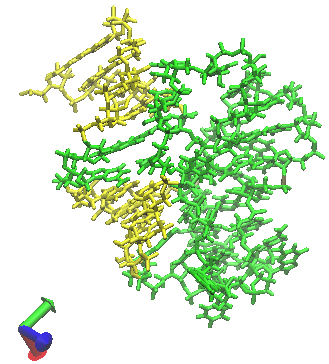
\includegraphics[scale=0.8]{./pictures/motifs_vmd.png}
\caption{The result of running the exemplary structure \texttt{vmd\_run.tcl} script in the VMD program after changing the display into \texttt{Orthographic} and the background color to white.}
\end{figure}

\subsection{Representing hydrogen bonding and stacking on the tertiary structure} 
The MINT program outputs several PDB files each with the B-factor column  replaced for each nucleotide atom line with:
\begin{itemize}
\item \texttt{\_WC.pdb} -- the number of hydrogen bonds in the WC pairs created by a given nucleotide.
\item \texttt{\_non-WC.pdb} -- the number of hydrogen bonds in the non-WC pairs created by a given nucleotide.
\item \texttt{\_coulomb.pdb} -- the Coulomb energy for a given nucleotide  (the sum of all electrostatic interactions the nucleotide is involved in).
\item \texttt{\_VDW.pdb} -- the Van der Waals energy for a given nucleotide (the sum of all interactions the nucleotide is involved in).
\item \texttt{\_stacking\_sum.pdb} -- the sum of the Van der Waals and Coulomb energies. 
\end{itemize}

For a trajectory these PDB files contain the average values (over all frames). Here, we only describe how to visualize the data outputted by MINT using VMD or Chimera.

\paragraph{VMD}
\texttt{VMD} is a powerful tool with a complete user guide and tutorial that can be found at (\url{http://www.ks.uiuc.edu/Research/vmd/}).
First, the user has to open the \texttt{VMD} program and load one of the PDB files, by choosing the \texttt{New Molecule} from the \texttt{File} drop-down menu as shown below:

\begin{figure}[h!]
\centering
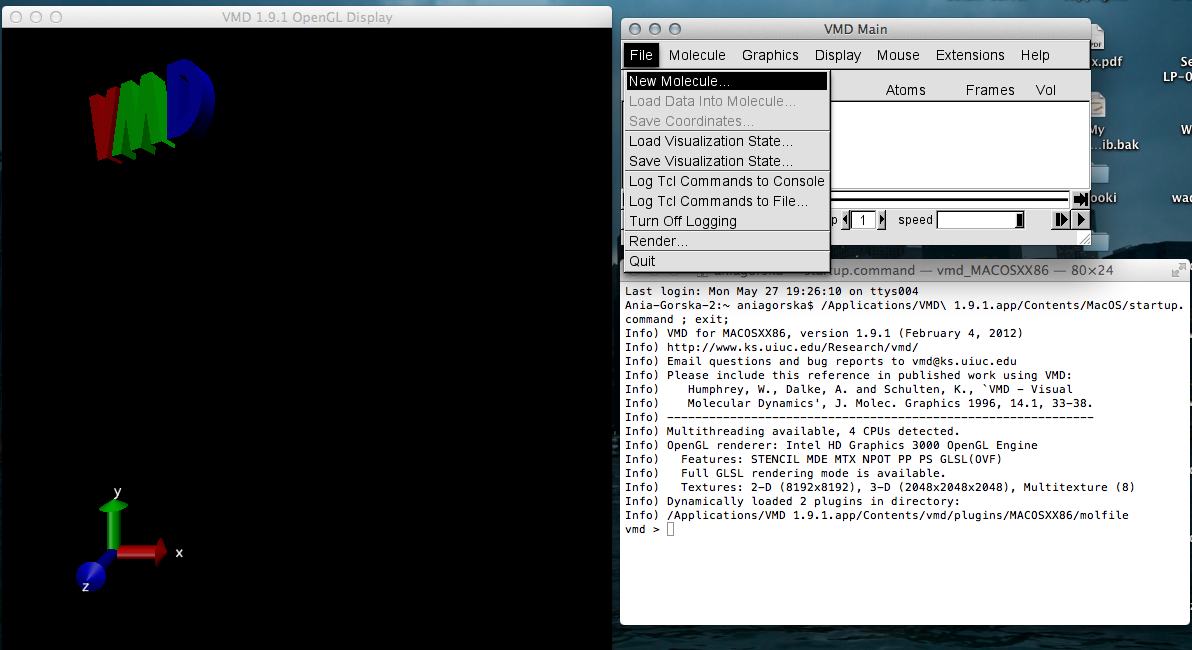
\includegraphics[scale=0.4]{./pictures/vmd1.png}
\caption{Loading a pdb file into the VMD program}
\end{figure}

Second, one has to \texttt{Browse} and \texttt{Load} a PDB file of choice:
\begin{figure}[h!]
\centering
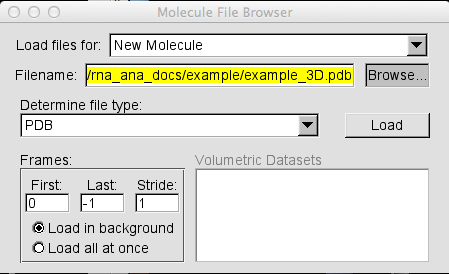
\includegraphics[scale=0.4]{./pictures/vmd2.png}
\caption{Loading a pdb file into VMD program}
\end{figure}
\newpage
Having uploaded the structure, one needs to open the \texttt{Representations} window from the \texttt{Graphics} drop-down menu:
\begin{figure}[h!]
\centering
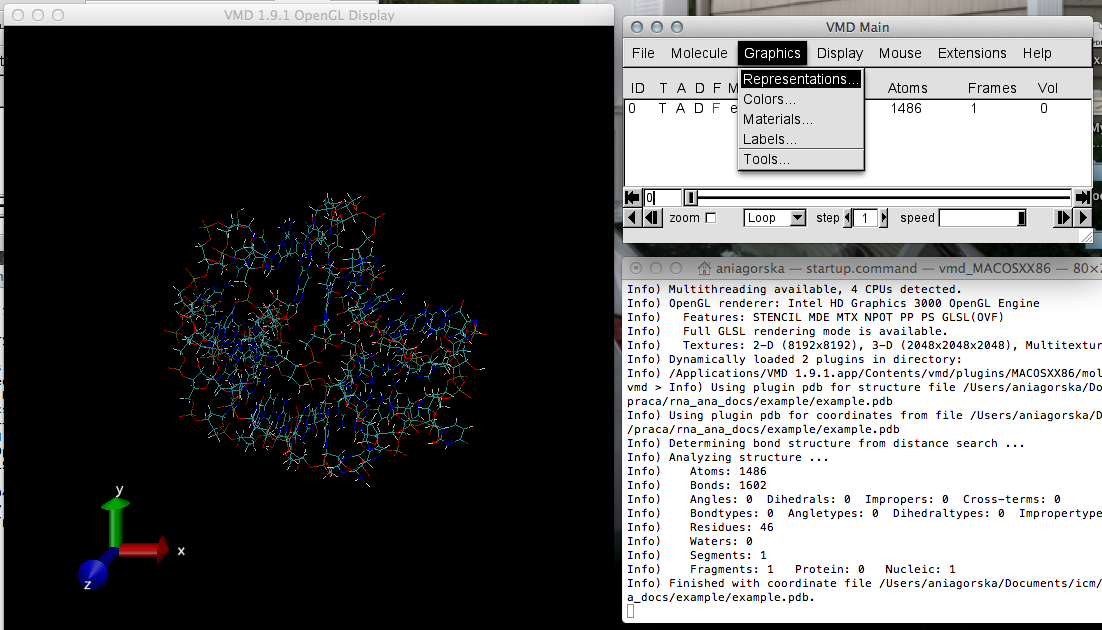
\includegraphics[scale=0.4]{./pictures/vmd3.png}
\caption{Opening the representation window in VMD}
\end{figure}

The \texttt{Representations} menu allows one to create various representations. To color the structure by the B-factor column in the PDB file, we suggest to change the \texttt{Drawing Methods} into the \texttt{New Cartoon} and the \texttt{Coloring Method} into the \texttt{Beta}:

\begin{figure} [h!]
\begin{center}
\subfigure[]{
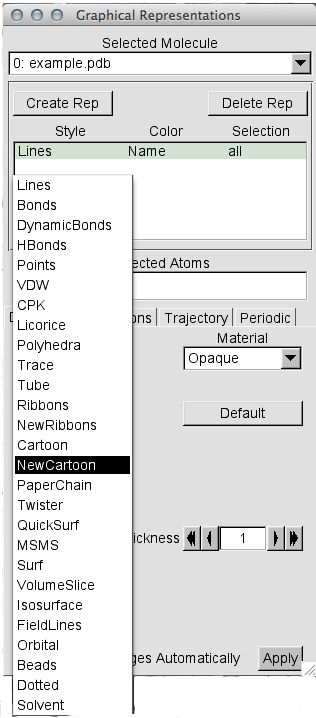
\includegraphics[scale=0.325]{pictures/vmd4.png}}
\subfigure[]{
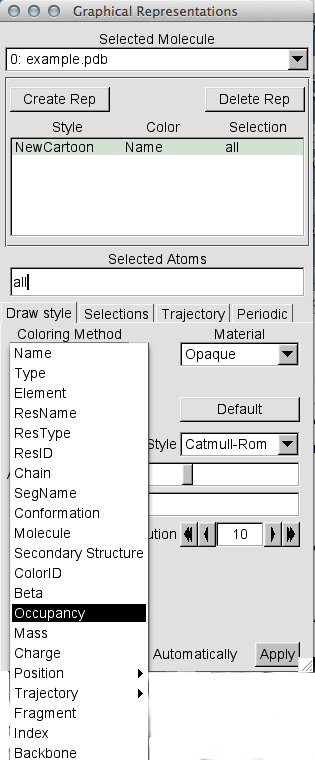
\includegraphics[scale=0.3]{pictures/vmd5.png}}
\end{center}
\caption{Choosing \texttt{Drawing} and \texttt{Color Methods} in the VMD program}
\end{figure} 

\newpage
Next, the color scale can be altered through \texttt{Graphics} $>$ \texttt{Color} $>$ \texttt{Color Scale}:

\begin{figure}[h!]
\centering
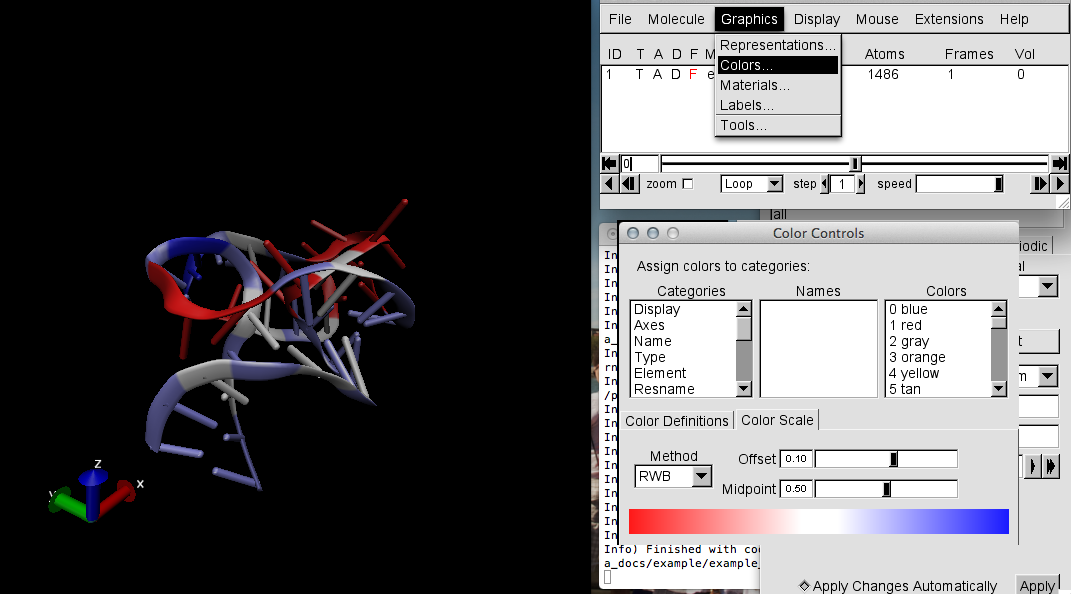
\includegraphics[scale=0.4]{./pictures/vmd6.png}
\caption{Changing the color scale}
\end{figure}

If you proceed in the same way with more than one PDB structure you can use the \texttt{Move} tool (\texttt{Mouse} $>$ \texttt{Move} $>$ \texttt{Molecule}) and view the colored structures at the same time as it is shown in Figure \ref{3Ddifferent}.

\begin{figure}[h!]
\centering
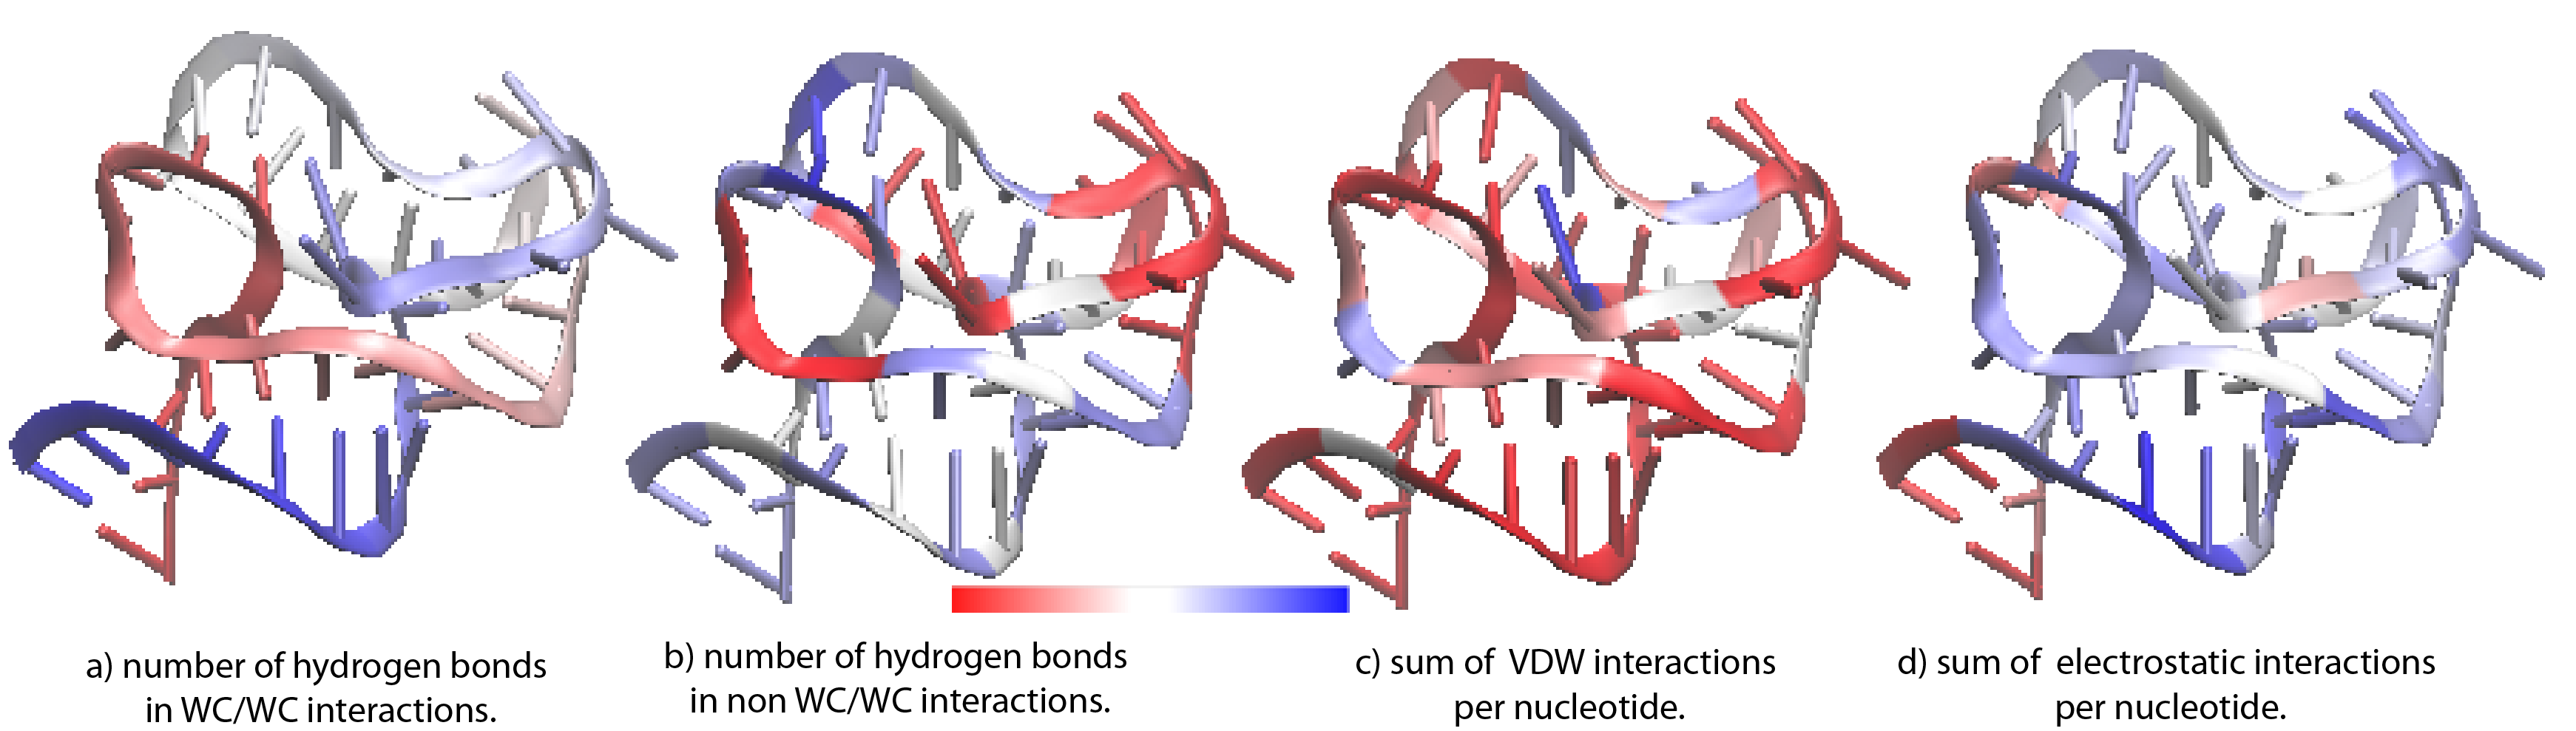
\includegraphics[scale=0.65]{./pictures/3D_different.png}
\caption{Exemplary pictures created with the use of the VMD program and the PDB files created by MINT. {\color{red} na tym rysunku nie ma jednostek energii, skali to jest chyba jakis stary rysunek.}}
\label{3Ddifferent}
\end{figure}

\paragraph{Chimera}
High-quality 3D visualizations can be also done with the {\tt Chimera} software (details on how to use the program can be found at (\url{https://www.cgl.ucsf.edu/chimera/}). The user has to open {\tt Chimera} and load one of the PDB files and next, choose from the \texttt{Tools} menu the \texttt{Depiction} section and click on the \texttt{Render by Attribute} as shown in Figure~\ref{chimera1}.

\begin{figure}[h!]
\centering
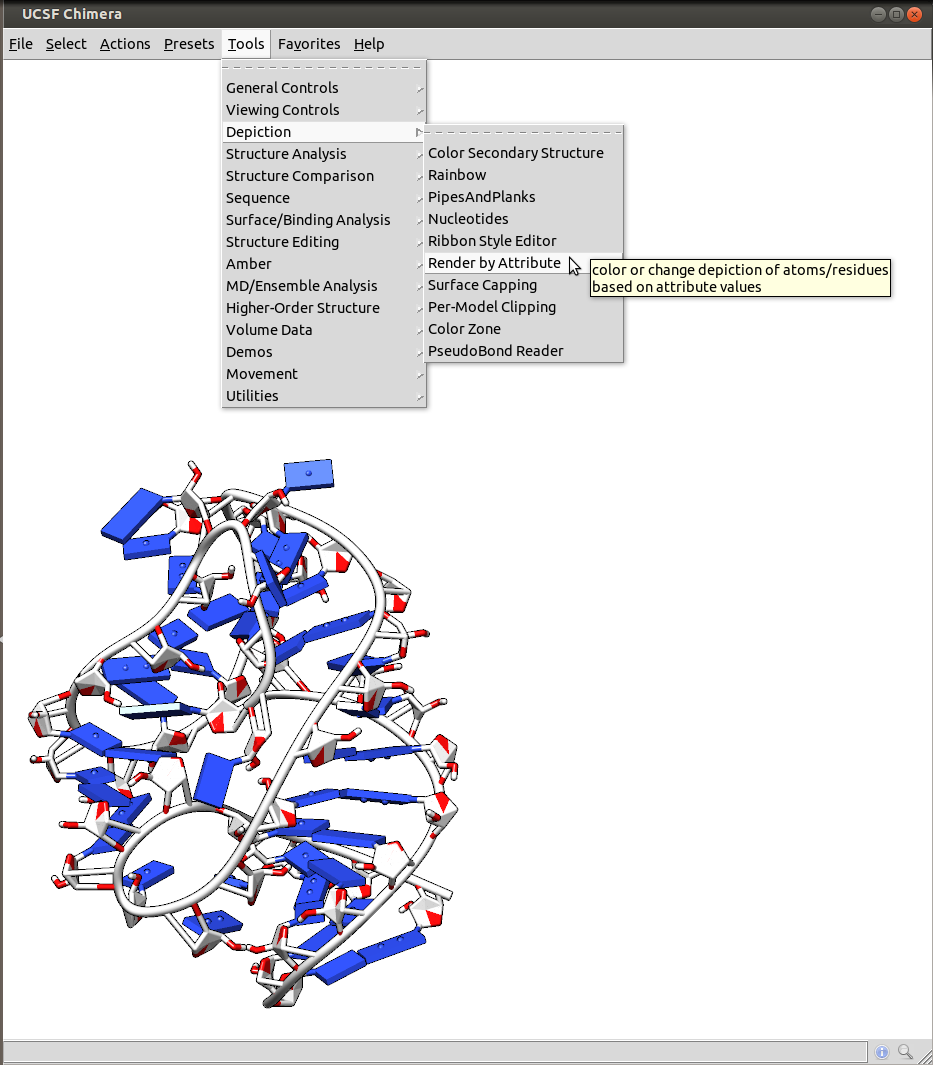
\includegraphics[scale=0.3]{./pictures/chimera1.png}
\caption{Render by attribute menu in Chimera}
\label{chimera1}
\end{figure}

In the opened window (Figure~\ref{chimera22}) the user chooses attributes of \texttt{residues} instead of default \texttt{atoms}. The \texttt{Attribute:} should be changed to \texttt{average -> bfactor}. Then the color scale and palette can be chosen and the color key can be created. Two exemplary pictures rendered in {\tt Chimera} are presented in Figure~\ref{chimera-pictures}.
\begin{figure}[!h]
\centering
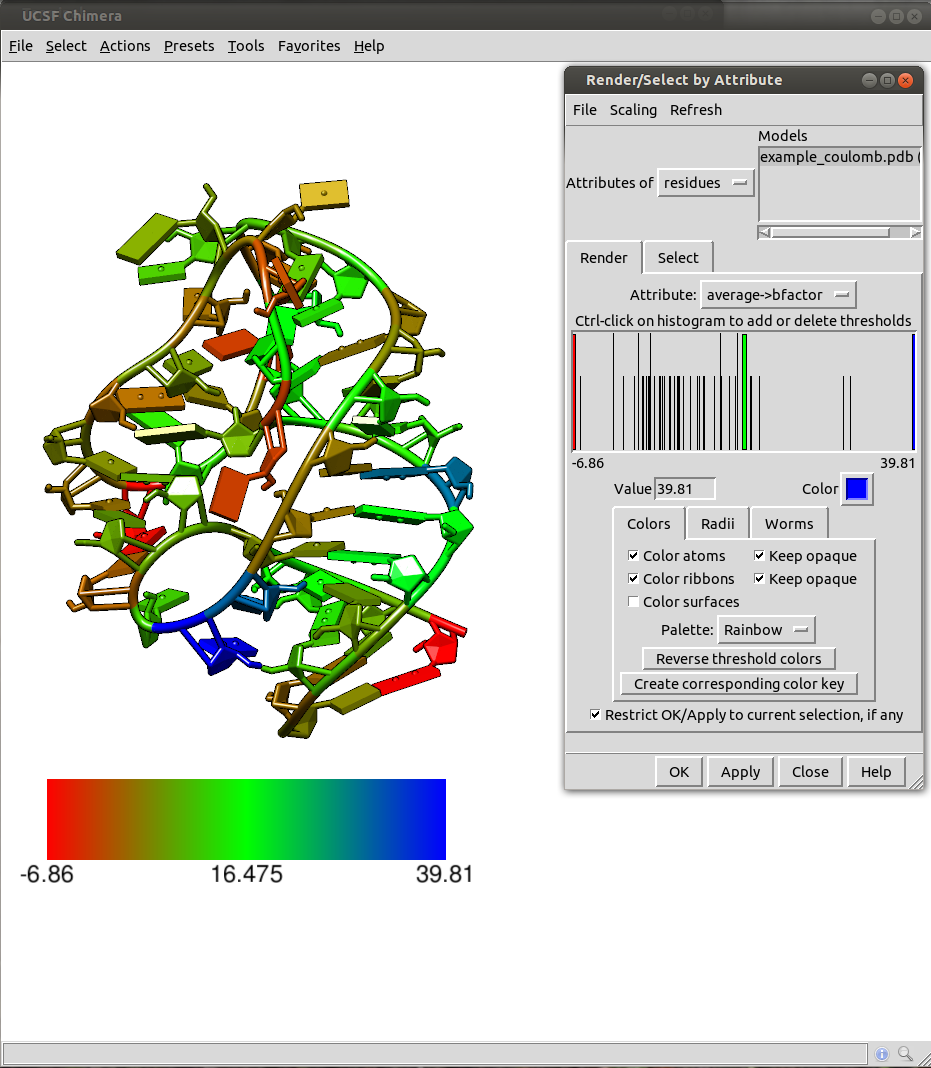
\includegraphics[scale=0.3]{./pictures/chimera2.png}
\caption{Rendering the structure by attribute in the Chimera program using the PDB file created by MINT}
\label{chimera22}
\end{figure}


\begin{figure}[!h]
%\centering
\hspace*{\fill}%
\subfigure[Average number of WC hydrogen bonds per nucleotide]{
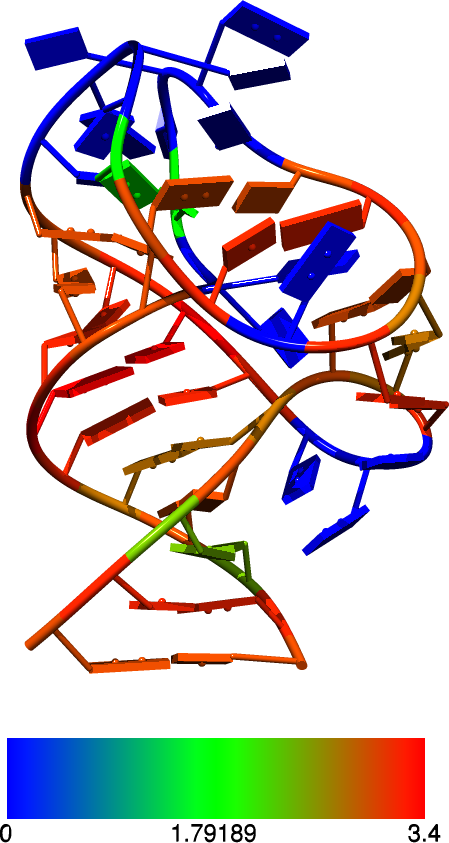
\includegraphics[scale=0.3]{./pictures/chimera-2D.png}}\hfill%
\subfigure[Average energy (in kcal/mol) of stacking interaction per nucleotide]{
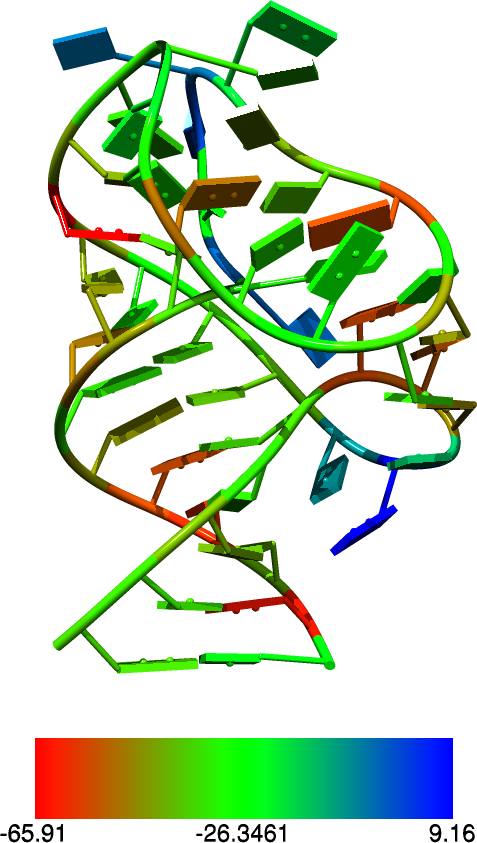
\includegraphics[scale=0.3]{./pictures/chimera-stacking.png}}
\hspace*{\fill}%
\caption{Exemplary pictures created with the use of the Chimera program and the PDB files created by MINT}
\label{chimera-pictures}
\end{figure}

\newpage
\subsection{Representing secondary structure changes} 
Analysed trajectory can be visualized in the secondary structure representation with the RNAMovies \cite{Evers1999} program. MINT returns the \texttt{RNAStructML.xml} file containing the trajectory of the secondary structure. For every frame the dot-bracket representation is written into the .xml file. This allows to produce the movie of the secondary structure trajectory. 

The RNAMovies \cite{Evers1999}  java .jar file can be downloaded from its home page: \url{http://bibiserv.techfak.uni-bielefeld.de/rnamovies/}. Here, we present a short tutorial on how to open an .xml file generated with MINT and view the secondary structure trajectory.

First, one has to open the RNAMovies and choose the \texttt{Import} option from the \texttt{File} drop-down menu. 
\begin{figure}[h!]
\centering
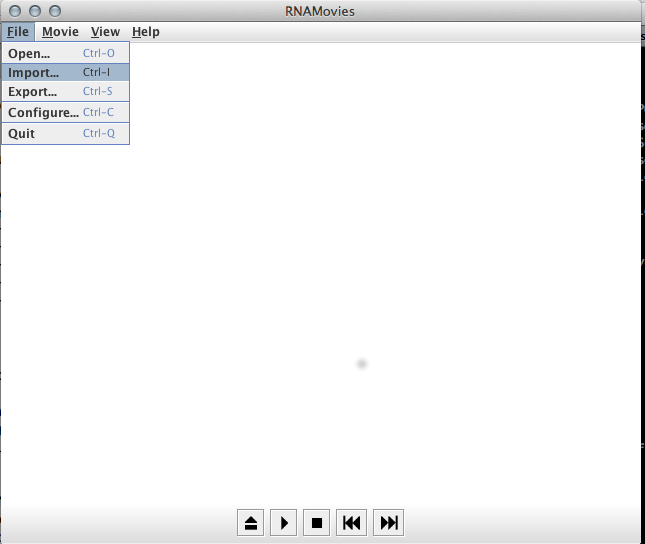
\includegraphics[scale=0.4]{./pictures/RNAmovies_1.png}
\end{figure}
\newpage
Find a proper .xml file in your directory, and click \texttt{Open}:
\begin{figure}[h!]
\centering
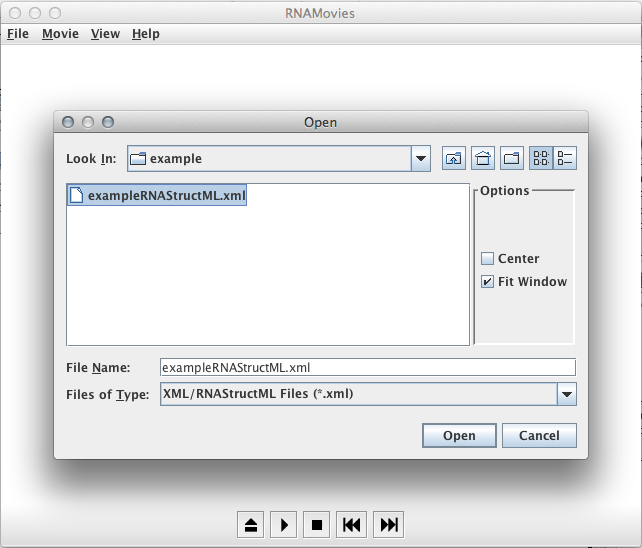
\includegraphics[scale=0.4]{./pictures/RNAmovies_2.png}
\end{figure}

One can navigate the trajectory using the arrows in the bottom of the window. If you would like to loop the trajectory or change the animation speed go to the \texttt{File} $>$ \texttt{Configure} menu: 
\begin{figure}[h!]
\centering
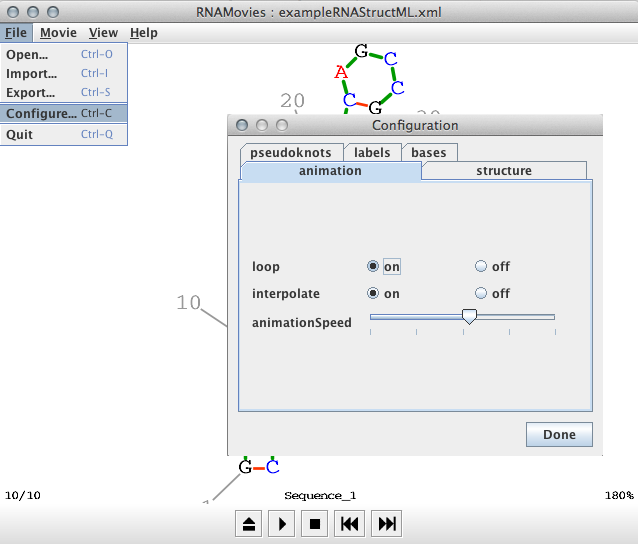
\includegraphics[scale=0.4]{./pictures/RNAmovies_3.png}
\end{figure}
\newpage
The animated trajectory can be written into the .gif file  (\texttt{File} $>$ \texttt{Export}).

\subsection{Correlations}\label{CorrelationsParagraph}
In the \texttt{MINT} directory there is an additional python script \texttt{CORRELATIONS.py} computing the $\phi$ coefficient for every pair of nucleotides in the structure. This coefficient is computed using the equation \cite{Everitt1977}:
\begin{center}
\begin{large}
$ \phi = \frac{n_{11}n_{00}}{\sqrt{n_{\bullet1}n_{\bullet0} n_{0\bullet}n_{1\bullet}}}$
\end{large}
\end{center}

where:
\begin{itemize}
\item $n_{11}$ is the number of frames in which both nucleotides form a WC pair.
\item $n_{00}$ is the number of frames in which none of the nucleotides forms a WC pair.
\item $n_{01}$ is the number of frames in which the first nucleotide forms a WC pair and the second nucleotide does not, analogously $n_{10}$ is the number of frames in which the first nucleotide is paired and the second one is unpaired.
\end{itemize}

and:
\begin{itemize}
\item $n_{\bullet1} = n_{11}+n_{01}$
\item $n_{1\bullet} = n_{11}+n_{10}$
\item $n_{\bullet0} = n_{00}+n_{10}$
\item $n_{0\bullet} = n_{00}+n_{01}$
\end{itemize}

\begin{figure}[h!]
\label{coefficient}
\centering
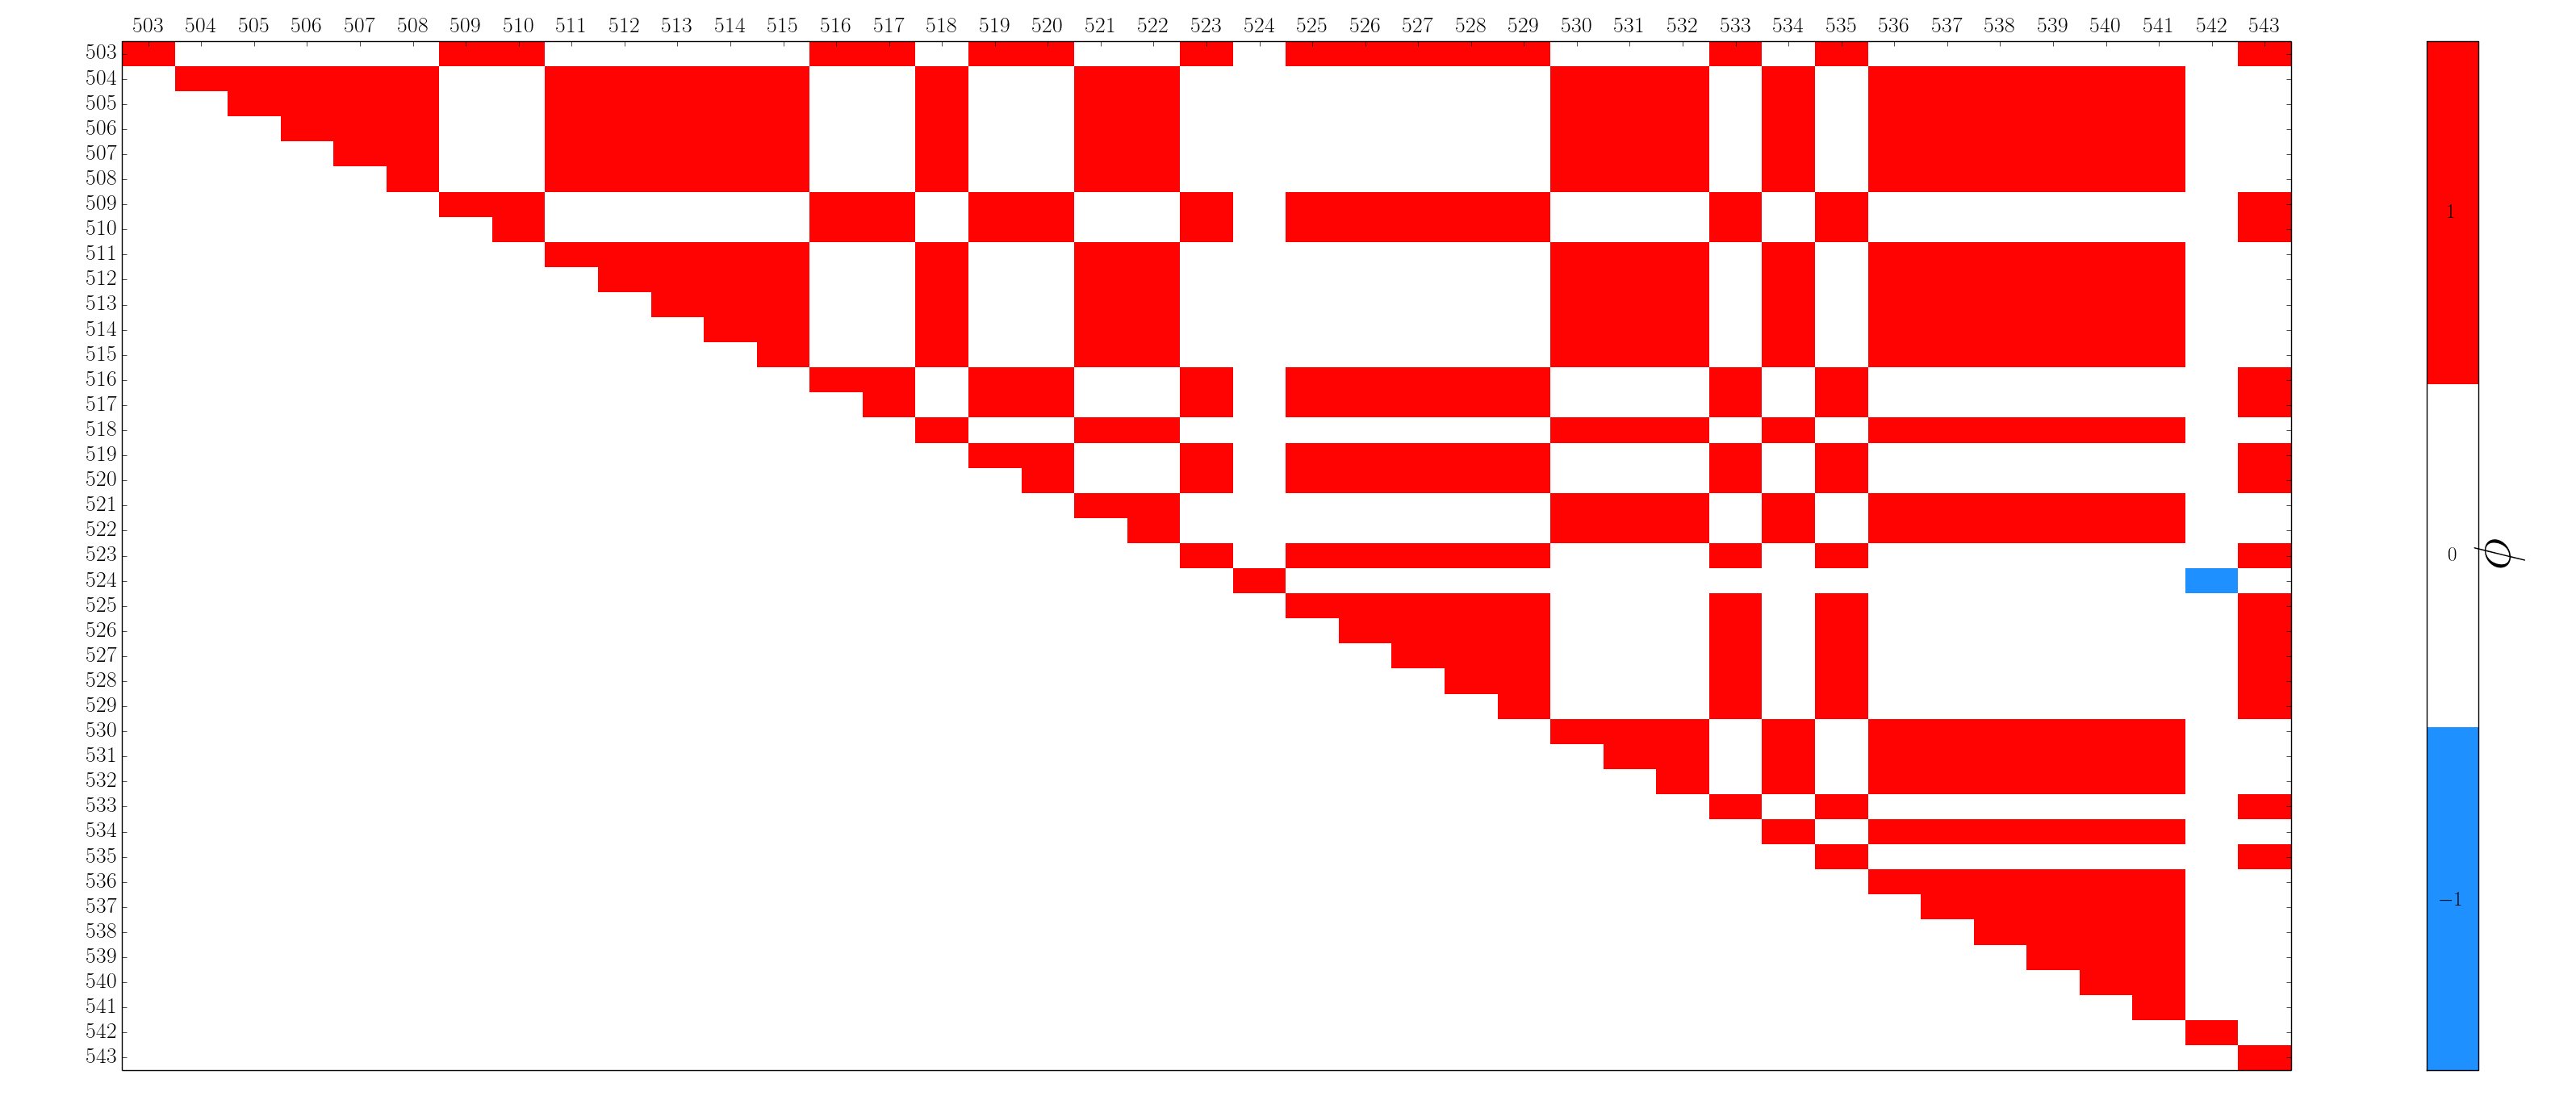
\includegraphics[scale=0.4]{./pictures/correlation_matrix.png}
\caption{Heat map of the $\phi$ coefficient for the the same exemplary molecule as shown before, {\color{red} gdzie before, na ktorym rysunku?}. The map was calculated with 0.4 \texttt{cutoff}.}
\end{figure}

The $\phi$ coefficient takes the values between $-1$ and $1$. If the value is close to $0$ the correlation is not reliable. In the heat map, all values larger than the \texttt{cutoff} will be marked red, all lower than \texttt{-1*cutoff} are marked blue. The rest will remain white. The level of \texttt{cutoff} is defined by the user.

The script produces a matrix that is both written into the text file and printed in the form of the heat map. Figure \ref{coefficient} {\color{red}  to jest rysunek 28 a nie sekcja 8.4} presents the heat map of the $\phi$ coefficient for an exemplary RNA molecule and its 10 frame-long molecular dynamics. The \texttt{CORRELATIONS.py} script uses as an input: the \texttt{MINT} output \texttt{pairs\_in\_time.csv} type, the cutoff and list of the numbers of nucleotides you would like to compute this coefficient for.

To compute the $\phi$ coefficient for all nucleotides type:
\begin{verbatim}
python CORRELATIONS.py filename_pairs_in_time.csv 0.4
\end{verbatim}
where \texttt{filename} is name of your csv file and \texttt{0.4} is an example of the \texttt{cutoff} for these calculations.
To compute the phi coefficient only for specified nucleotides type:\\

\begin{verbatim}
python CORRELATIONS.py filename_pairs_in_time.csv 0.4 "[(1210,1220),(985,995)]" 
\end{verbatim}

The list of nucleotides has to be specified in square brackets and quotation marks. Inside the round brackets the ranges of nucleotides must be specified. 

The heat map is only printed for the half of the matrix because the matric is symmetric and the other half is identical. All nucleotides are correlated with themselves so the diagonal is red. All nucleotides that form the WC pairs with each other are also positively correlated. The neighbouring pairs that work together will be also correlated in all to all manner. The negative correlation suggests that there are pairs that open while others close.

\section{Appendices}
\begin{appendices}
\subsection{Adding hydrogens to a PDB structure}
The hydrogen bond definition used in {\tt MINT} requires hydrogen atoms in the structure in order to measure the angle. Therefore, the input file has to contain all atoms.

If one analyzes the trajectory files derived from MD simulations, the hydrogen atoms were added to the structure during the preparation of an MD run, according to the atom type definitions in the used force field. Various tools from the MD packages can be used to assign the positions of hydrogens (for example, Xleap from AmberTools). 

However, if a structure from the PDB database has to be analyzed and the user does not have experience with the MD methods, hydrogen atoms can be added using on-line servers. We have tested a few and recommend the {\tt Molprobility} service~\cite{Chen2010} (\url{http://molprobity.biochem.duke.edu/}). It works even with the structures as large as the ribosomal subunits in an acceptable time span. What is more, the software can be downloaded from the \url{http://kinemage.biochem.duke.edu/software/reduce.php} website and used offline.

{\color{red}If you use the MINT web server for a single conformation the positions of hydrogens will be automatically added to the PDB file by the reduce program .....}

\subsection{Exemplary description file}
A fragment of the \texttt{\_description} file generated during the analysis of an \texttt{example.dcd} trajectory.
\begin{scriptsize}
\begin{lstlisting}
Running with parameters: 
cutoff=20.0
file_name=1e8o/1e8o_H.pdb
vmd=1
h_bond_l=4.0
MINT_home=/Users/agorska/Documents/mint
SingleOrTraj=Single
max_memory_GB=1.5
table_charges=/Users/agorska/Documents/mint/data/charges_and_VDW_modified.csv
vdw_cutoff_stacking=0.0
h_bond_atom=donor
list_of_modified_nucs=data/unknown_modified.fa
only_analysis=0
h_bond_angle=140.0
force_field=AMBER
pdb_list=
chains_names=[]
cutoff_stacking=10.5
table_nucleotides=/Users/agorska/Documents/mint/data/nucleotides_modified.csv
margin=0.8
OP_stacking_distance_cutoff=4.5

  50 nucleotides, sequence: 
GDP G G C C G G G C G C G G U G G C G C G C G C C U G U A G U C C C A G C U A C U C G G G A G G C U C 
Nucleotides statistics:
GDP-> 1 UNknown parameters
A  -> 4 known parameters
C  -> 17 known parameters
U  -> 7 known parameters
G  -> 21 known parameters

Stacking pairs
 qn1 n2     Coul     VdW    sum
E|GDP:99 E|G:100 MODIFIED NUCLEOTIDES
E|G:100 E|G:101(6.81, -29.13, -22.32)
E|G:100 E|C:148(0.87, -15.41, -14.54)
E|G:101 E|C:102(-5.15, -27.25, -32.4)
E|G:101 E|U:147(2.39, -8.82, -6.43)
E|G:101 E|C:148(1.21, -0.83, 0.38)
E|C:102 E|C:103(2.45, -16.48, -14.04)
E|C:102 E|G:104(0.29, -0.01, 0.27)
E|C:102 E|G:127(-0.46, -0.17, -0.63)
E|C:102 E|C:146(7.14, -3.61, 3.52)
E|C:102 E|U:147(0.04, -0.48, -0.44)
E|C:103 E|G:104(0.43, -0.05, 0.38)
E|C:103 E|U:125(0.89, -0.04, 0.86)
E|C:103 E|G:127(0.58, -0.23, 0.36)
E|C:103 E|U:128(-0.18, -16.47, -16.64)
E|C:103 E|G:145(0.78, -12.04, -11.26)
E|C:103 E|C:146(-0.29, -0.68, -0.97)
E|G:104 E|G:105(4.39, -28.74, -24.36)
E|G:104 E|G:124(10.25, -47.13, -36.88)
E|G:104 E|U:125(1.61, -1.07, 0.55)
E|G:104 E|G:127(0.33, -0.07, 0.26)
E|G:104 E|U:128(0.26, -0.06, 0.2)
E|G:105 E|G:106(4.16, -33.32, -29.16)
E|G:105 E|U:123(-0.56, -18.01, -18.57)
E|G:105 E|G:124(2.04, -1.12, 0.92)
E|G:106 E|C:107(-6.13, -24.33, -30.46)
E|G:106 E|C:122(2.58, -23.41, -20.83)
E|G:106 E|U:123(1.66, -1.16, 0.5)
E|C:107 E|G:108(0.59, -13.24, -12.65)
E|C:107 E|C:109(0.41, -0.43, -0.02)
E|C:107 E|C:121(11.13, -3.72, 7.41)
E|C:107 E|C:122(-0.07, -0.63, -0.7)
E|G:108 E|C:109(-6.12, -33.9, -40.03)
E|G:108 E|G:120(3.94, -42.7, -38.77)
E|G:108 E|C:121(1.46, -1.07, 0.39)
E|C:109 E|G:110(-0.23, -15.2, -15.43)
E|C:109 E|C:119(7.69, -3.49, 4.2)
E|C:109 E|G:120(1.4, -1.12, 0.28)
E|G:110 E|G:111(5.9, -31.9, -26.0)
E|G:110 E|G:118(4.06, -37.12, -33.06)
E|G:110 E|C:119(0.64, -1.08, -0.44)
E|G:111 E|U:112(5.24, -29.22, -23.97)
E|G:111 E|C:117(-0.67, -21.94, -22.61)
E|G:111 E|G:118(1.57, -1.25, 0.32)
E|U:112 E|G:113(1.15, -0.46, 0.69)
E|U:112 E|G:114(2.86, -6.99, -4.14)
E|U:112 E|C:115(-2.71, -6.24, -8.95)
E|U:112 E|G:116(1.37, -0.44, 0.94)
E|U:112 E|C:117(-0.39, -0.55, -0.94)
E|G:113 E|G:114(5.67, -24.04, -18.36)
E|G:113 E|A:136(10.23, -43.78, -33.55)
E|G:114 E|C:115(-6.38, -32.43, -38.81)
E|G:114 E|G:116(2.02, -0.71, 1.31)
E|G:114 E|U:135(1.6, -1.35, 0.24)
E|G:114 E|A:136(4.33, -1.03, 3.3)
E|G:114 E|C:137(3.09, -19.27, -16.18)
E|G:114 E|U:138(0.04, -0.04, 0.0)
E|C:115 E|G:116(-0.95, -19.76, -20.71)
E|C:115 E|C:117(-0.63, -0.57, -1.19)
E|C:115 E|C:134(7.47, -5.28, 2.19)
E|C:115 E|C:137(-1.16, -0.67, -1.83)
E|C:115 E|U:138(0.34, -0.03, 0.31)
E|C:115 E|C:139(0.7, -0.04, 0.66)
E|C:115 E|G:140(1.06, -0.33, 0.73)
E|G:116 E|C:117(3.24, -8.55, -5.32)
E|G:116 E|G:133(-0.57, -19.77, -20.34)
E|G:116 E|C:134(0.92, -0.9, 0.02)
E|G:116 E|G:140(1.06, -0.84, 0.22)
E|C:117 E|G:118(1.3, -6.89, -5.58)
E|C:117 E|A:132(1.29, -0.2, 1.09)
E|C:117 E|G:133(1.48, -0.17, 1.31)
E|G:118 E|C:119(-7.54, -32.27, -39.81)
E|C:119 E|G:120(0.73, -12.44, -11.71)
E|C:119 E|C:121(0.96, -0.44, 0.53)
E|G:120 E|C:121(-5.61, -29.68, -35.29)
E|C:121 E|C:122(3.12, -11.4, -8.28)
E|C:122 E|U:123(0.19, -20.38, -20.2)
E|U:123 E|G:124(1.36, -2.12, -0.76)
E|G:124 E|U:125(3.46, -30.35, -26.89)
E|U:125 E|A:126(3.37, -0.33, 3.04)
E|U:125 E|G:127(3.19, -6.0, -2.8)
E|A:126 E|G:127(8.62, -38.42, -29.8)
E|G:127 E|U:128(0.05, -0.05, 0.0)
E|G:127 E|G:145(0.37, -0.32, 0.05)
E|G:127 E|C:146(-1.62, -0.32, -1.94)
E|U:128 E|C:130(0.02, -0.44, -0.41)
E|U:128 E|G:144(3.01, -11.17, -8.16)
E|U:128 E|G:145(1.34, -0.8, 0.54)
E|C:129 E|C:130(2.97, -18.79, -15.82)
E|C:129 E|A:143(7.27, -17.4, -10.13)
E|C:129 E|G:144(1.02, -1.08, -0.06)
E|C:130 E|C:131(3.16, -15.29, -12.14)
E|C:130 E|G:142(1.14, -15.47, -14.33)
E|C:130 E|A:143(1.97, -1.13, 0.84)
E|C:130 E|G:144(0.52, -0.12, 0.41)
E|C:131 E|A:132(2.89, -15.5, -12.61)
E|C:131 E|G:133(0.45, -0.2, 0.25)
E|C:131 E|G:141(1.37, -16.36, -14.99)
E|C:131 E|G:142(1.2, -0.93, 0.26)
E|A:132 E|G:133(2.81, -9.56, -6.75)
E|A:132 E|C:134(0.78, -0.24, 0.54)
E|A:132 E|G:140(6.69, -19.25, -12.56)
E|A:132 E|G:141(3.66, -1.05, 2.61)
E|G:133 E|C:134(-7.87, -35.35, -43.22)
E|G:133 E|U:135(1.52, -0.88, 0.64)
E|G:133 E|G:140(2.11, -6.55, -4.45)
E|G:133 E|G:141(0.2, -0.22, -0.02)
E|C:134 E|U:135(-1.29, -19.98, -21.28)
E|C:134 E|C:137(-2.76, -5.1, -7.86)
E|C:134 E|C:139(0.64, -0.04, 0.6)
E|C:134 E|G:140(0.27, -0.54, -0.27)
E|C:134 E|G:141(0.48, -0.05, 0.44)
E|U:135 E|A:136(4.73, -0.52, 4.22)
E|U:135 E|C:137(-1.41, -2.63, -4.04)
E|U:135 E|G:140(0.33, -0.06, 0.27)
E|A:136 E|C:137(4.25, -4.69, -0.43)
E|C:137 E|U:138(0.38, -0.03, 0.35)
E|C:137 E|C:139(-1.22, -0.72, -1.94)
E|U:138 E|C:139(-0.63, -0.2, -0.83)
E|C:139 E|G:140(0.2, -0.03, 0.17)
E|G:140 E|G:141(5.9, -26.62, -20.71)
E|G:141 E|G:142(5.16, -24.28, -19.12)
E|G:142 E|A:143(6.88, -32.19, -25.31)
E|A:143 E|G:144(9.52, -22.79, -13.27)
E|G:144 E|G:145(7.87, -33.17, -25.3)
E|G:145 E|C:146(-7.61, -36.56, -44.17)
E|G:145 E|U:147(1.22, -0.74, 0.48)
E|C:146 E|U:147(-0.68, -21.82, -22.5)
E|U:147 E|C:148(-0.28, -11.16, -11.44)

Helices: 
1] E|G:100-E|C:103 -> E|G:144-E|U:147
2] E|U:128-E|C:131 -> E|G:140-E|A:143
Helices vmd
1] chain E and resid 100 to 103  chain E and resid 144 to 147
2] chain E and resid 128 to 131  chain E and resid 140 to 143

Pseudoknots:
E|G:105-E|C:122 E|G:106-E|C:121 E|C:107-E|G:120 E|G:108-E|C:119 E|C:109-E|G:118 E|G:110-
E|C:117 E|G:113-E|C:137 E|G:114-E|C:134 E|C:115-E|G:133 
Pseudoknots vmd
chain E and resid  105 122 106 121 107 120 108 119 109 118 110 117 113 137 114 134 115 133 

Motifs:
1]  0-24  E|C:103-E|G:144-E|A:143-E|U:128-E|G:127-E|A:126-E|U:125-E|G:124-E|U:123-
E|C1:22-E|C:121-E|G:120-E|C:119-E|G:118-E|C:117-E|G:116-E|C:115-E|G:114-E|G:113-
E|U:112-E|G:111-E|G:110-E|C:109-E|G:108-E|C:107-E|G:106-E|G:105-E|G:104-E|C:103-
2]  8  E|C:131-E|G:140-E|C:139-E|U:138-E|C:137-E|A:136-E|U:135-E|C:134-E|G:133-
E|A:132-E|C:131-

Motifs vmd
1]  chain E and resid  103 144 143 128 127 126 125 124 123 122 121
120 119 118 117 116 115 114 113 112 111 110 109 108 107 106 105 104 103 
2]  chain E and resid  131 140 139 138 137 136 135 134 133 132 131 


WC Base pairs: 
0] E|G:100/E|U:147  N1-H1-O2 angle: 173.74 distance: 3.93  | O6-H3-N3 angle: 163.32  distance: 3.79 WC/WC/2  Cis
1] E|G:101/E|C:146  N2-H22-O2 angle: 166.42 distance: 4.12  | N1-H1-O2 angle: 146.26 distance: 4.37  | N1-H1-N3 angle: 157.94 distance: 4.0  | O6-H42-N4 angle: 157.36 distance: 3.82 WC/WC/4  Cis
2] E|C:102/E|G:145  N4-H42-O6 angle: 176.26 distance: 4.49  | O2-H22-N2 angle: 161.57 distance: 3.72  | N3-H22-N2 angle: 143.38 distance: 4.45  | N3-H1-N1 angle: 170.35 distance: 4.18 WC/WC/4  Cis
3] E|C:103/E|G:144  N4-H42-O6 angle: 158.55 distance: 3.85  | O2-H22-N2 angle: 163.22 distance: 3.78  | N3-H1-N1 angle: 168.86 distance: 3.9 WC/WC/3  Cis
4] E|G:105/E|C:122  N2-H22-O2 angle: 175.58 distance: 3.69  | N1-H1-N3 angle: 169.81 distance: 4.04  | O6-H42-N4 angle: 162.42 distance: 4.26 WC/WC/3  Cis
5] E|G:106/E|C:121  N2-H22-O2 angle: 146.21 distance: 3.89  | N1-H1-N3 angle: 157.79 distance: 4.02  | O6-H42-N4 angle: 143.78 distance: 3.89 WC/WC/3  Cis
6] E|C:107/E|G:120  N4-H42-O6 angle: 162.89 distance: 3.96  | O2-H22-N2 angle: 162.01 distance: 3.74  | N3-H1-N1 angle: 161.54 distance: 3.91 WC/WC/3  Cis
7] E|G:108/E|C:119  N2-H22-O2 angle: 166.35 distance: 3.75  | N1-H1-N3 angle: 177.38 distance: 3.94  | O6-H42-N4 angle: 176.92 distance: 3.99 WC/WC/3  Cis
8] E|C:109/E|G:118  N4-H42-O6 angle: 178.08 distance: 4.16  | O2-H22-N2 angle: 168.71 distance: 3.81  | N3-H1-N1 angle: 176.03 distance: 4.05 WC/WC/3  Cis
9] E|G:110/E|C:117  N2-H22-O2 angle: 175.9 distance: 3.97  | N1-H1-N3 angle: 173.38 distance: 3.99  | O6-H42-N4 angle: 151.62 distance: 3.79 WC/WC/3  Cis
10] E|G:113/E|C:137  N2-H22-O2 angle: 161.78 distance: 3.87  | N2-H22-N3 angle: 140.43 distance: 4.3  | N1-H1-N3 angle: 167.06 distance: 4.01  | O6-H42-N4 angle: 168.21 distance: 3.99 WC/WC/4  Cis
11] E|G:114/E|C:134  N2-H22-O2 angle: 166.07 distance: 3.82  | N1-H1-O2 angle: 140.14 distance: 4.13  | N1-H1-N3 angle: 158.62 distance: 4.03  | O6-H42-N4 angle: 155.35 distance: 4.16 WC/WC/4  Cis
12] E|C:115/E|G:133  N4-H42-O6 angle: 148.46 distance: 4.11  | O2-H22-N2 angle: 152.84 distance: 3.9  | N3-H1-N1 angle: 160.16 distance: 4.05 WC/WC/3  Cis
13] E|U:128/E|A:143  N3-H3-N1 angle: 175.56 distance: 4.17  | N3-H3-C2 angle: 155.22 distance: 4.79  | O4-H61-N6 angle: 165.29 distance: 4.5 WC/WC/3  Cis
14] E|C:129/E|G:142  N4-H42-O6 angle: 163.69 distance: 4.26  | O2-H22-N2 angle: 164.72 distance: 3.81  | N3-H22-N2 angle: 141.13 distance: 4.44  | N3-H1-N1 angle: 174.06 distance: 4.12 WC/WC/4  Cis
15] E|C:130/E|G:141  N4-H42-O6 angle: 169.64 distance: 4.03  | O2-H22-N2 angle: 153.16 distance: 3.61  | N3-H22-N2 angle: 142.65 distance: 4.08  | N3-H1-N1 angle: 164.36 distance: 3.9 WC/WC/4  Cis
16] E|C:131/E|G:140  N4-H42-O6 angle: 164.81 distance: 4.08  | O2-H22-N2 angle: 173.16 distance: 3.87  | N3-H1-N1 angle: 167.41 distance: 4.02 WC/WC/3  Cis

Other interactions: 
0] E|GDP:99/E|C:148  C6-H42-N4 angle: 167.04 distance: 4.46  | O6-H42-N4 angle: 164.14
 distance: 3.8 W?H/WC/2  Cis
1] E|G:104/E|U:123  N1-H1-O2 angle: 149.85 distance: 3.86 WC/WC*Sugar/1  Cis
2] E|G:111/E|G:116  N2-H21-O6 angle: 153.07 distance: 3.88 WC*Sugar/WC*Hoogsteen/1  Trans
3] E|G:116/E|A:132  N2-H21-C2 angle: 153.51 distance: 4.64  | N2-H21-N3 angle: 167.69
 distance: 4.71 WC/Sugar/2  Trans
4] E|U:128/E|C:129  O2'-H6-C6 angle: 147.39 distance: 4.37 Sugar/Hoogsteen/1  Cis

Dot-Bracket
gGGCCGGGCGCGGUGGCGCGCGCCUGUAGUCCCAGCUACUCGGGAGGCUC
.((((........................((((........)))))))).
 Modified nucleotides denoted by lower case letters


Stacking pi pairs
E|U:125_E|G:127_OP2 4.02 (2.16, -7.04, -4.87)
E|U:112_E|G:114_OP2 4.21 (2.3, -6.31, -4.01)

\end{lstlisting}
\end{scriptsize}

\end{appendices}
\bibliography{bibliografia}
\bibliographystyle{plain}
\end{document}